\documentclass[twoside]{book}

% Packages required by doxygen
\usepackage{fixltx2e}
\usepackage{calc}
\usepackage{doxygen}
\usepackage[export]{adjustbox} % also loads graphicx
\usepackage{graphicx}
\usepackage[utf8]{inputenc}
\usepackage{makeidx}
\usepackage{multicol}
\usepackage{multirow}
\PassOptionsToPackage{warn}{textcomp}
\usepackage{textcomp}
\usepackage[nointegrals]{wasysym}
\usepackage[table]{xcolor}

% NLS support packages
\usepackage[T2A]{fontenc}
\usepackage[russian]{babel}

% Font selection
\usepackage[T1]{fontenc}
\usepackage[scaled=.90]{helvet}
\usepackage{courier}
\usepackage{amssymb}
\usepackage{sectsty}
\renewcommand{\familydefault}{\sfdefault}
\allsectionsfont{%
  \fontseries{bc}\selectfont%
  \color{darkgray}%
}
\renewcommand{\DoxyLabelFont}{%
  \fontseries{bc}\selectfont%
  \color{darkgray}%
}
\newcommand{\+}{\discretionary{\mbox{\scriptsize$\hookleftarrow$}}{}{}}

% Page & text layout
\usepackage{geometry}
\geometry{%
  a4paper,%
  top=2.5cm,%
  bottom=2.5cm,%
  left=2.5cm,%
  right=2.5cm%
}
\tolerance=750
\hfuzz=15pt
\hbadness=750
\setlength{\emergencystretch}{15pt}
\setlength{\parindent}{0cm}
\setlength{\parskip}{3ex plus 2ex minus 2ex}
\makeatletter
\renewcommand{\paragraph}{%
  \@startsection{paragraph}{4}{0ex}{-1.0ex}{1.0ex}{%
    \normalfont\normalsize\bfseries\SS@parafont%
  }%
}
\renewcommand{\subparagraph}{%
  \@startsection{subparagraph}{5}{0ex}{-1.0ex}{1.0ex}{%
    \normalfont\normalsize\bfseries\SS@subparafont%
  }%
}
\makeatother

% Headers & footers
\usepackage{fancyhdr}
\pagestyle{fancyplain}
\fancyhead[LE]{\fancyplain{}{\bfseries\thepage}}
\fancyhead[CE]{\fancyplain{}{}}
\fancyhead[RE]{\fancyplain{}{\bfseries\leftmark}}
\fancyhead[LO]{\fancyplain{}{\bfseries\rightmark}}
\fancyhead[CO]{\fancyplain{}{}}
\fancyhead[RO]{\fancyplain{}{\bfseries\thepage}}
\fancyfoot[LE]{\fancyplain{}{}}
\fancyfoot[CE]{\fancyplain{}{}}
\fancyfoot[RE]{\fancyplain{}{\bfseries\scriptsize Создано системой Doxygen }}
\fancyfoot[LO]{\fancyplain{}{\bfseries\scriptsize Создано системой Doxygen }}
\fancyfoot[CO]{\fancyplain{}{}}
\fancyfoot[RO]{\fancyplain{}{}}
\renewcommand{\footrulewidth}{0.4pt}
\renewcommand{\chaptermark}[1]{%
  \markboth{#1}{}%
}
\renewcommand{\sectionmark}[1]{%
  \markright{\thesection\ #1}%
}

% Indices & bibliography
\usepackage{natbib}
\usepackage[titles]{tocloft}
\setcounter{tocdepth}{3}
\setcounter{secnumdepth}{5}
\makeindex

% Hyperlinks (required, but should be loaded last)
\usepackage{ifpdf}
\ifpdf
  \usepackage[pdftex,pagebackref=true]{hyperref}
\else
  \usepackage[ps2pdf,pagebackref=true]{hyperref}
\fi
\hypersetup{%
  colorlinks=true,%
  linkcolor=blue,%
  citecolor=blue,%
  unicode%
}

% Custom commands
\newcommand{\clearemptydoublepage}{%
  \newpage{\pagestyle{empty}\cleardoublepage}%
}

\usepackage{caption}
\captionsetup{labelsep=space,justification=centering,font={bf},singlelinecheck=off,skip=4pt,position=top}

%===== C O N T E N T S =====

\begin{document}

% Titlepage & ToC
\hypersetup{pageanchor=false,
             bookmarksnumbered=true,
             pdfencoding=unicode
            }
\pagenumbering{alph}
\begin{titlepage}
\vspace*{7cm}
\begin{center}%
{\Large Radix }\\
\vspace*{1cm}
{\large Создано системой Doxygen 1.8.13}\\
\end{center}
\end{titlepage}
\clearemptydoublepage
\pagenumbering{roman}
\tableofcontents
\clearemptydoublepage
\pagenumbering{arabic}
\hypersetup{pageanchor=true}

%--- Begin generated contents ---
\chapter{Алфавитный указатель пространств имен}
\section{Пространства имен}
Полный список пространств имен.\begin{DoxyCompactList}
\item\contentsline{section}{\hyperlink{namespacelogo}{logo} }{\pageref{namespacelogo}}{}
\item\contentsline{section}{\hyperlink{namespacemenu}{menu} }{\pageref{namespacemenu}}{}
\item\contentsline{section}{\hyperlink{namespaceradix}{radix} }{\pageref{namespaceradix}}{}
\end{DoxyCompactList}

\chapter{Алфавитный указатель классов}
\section{Классы}
Классы с их кратким описанием.\begin{DoxyCompactList}
\item\contentsline{section}{\hyperlink{structmenu__s}{menu\+\_\+s} }{\pageref{structmenu__s}}{}
\end{DoxyCompactList}

\chapter{Список файлов}
\section{Файлы}
Полный список файлов.\begin{DoxyCompactList}
\item\contentsline{section}{\hyperlink{_a_d_b__mod_8cpp}{A\+D\+B\+\_\+mod.\+cpp} \\*Модуль работы с adb }{\pageref{_a_d_b__mod_8cpp}}{}
\item\contentsline{section}{\hyperlink{_a_d_b__mod_8h}{A\+D\+B\+\_\+mod.\+h} \\*Заголовочный файл с подключением модуля работы с adb }{\pageref{_a_d_b__mod_8h}}{}
\item\contentsline{section}{\hyperlink{_color_8cpp}{Color.\+cpp} \\*Модуль работы с цветом в консоли }{\pageref{_color_8cpp}}{}
\item\contentsline{section}{\hyperlink{_color_8h}{Color.\+h} \\*Заголовочный файл с цветами и модулем смены цвета в консоли }{\pageref{_color_8h}}{}
\item\contentsline{section}{\hyperlink{_constants_8h}{Constants.\+h} \\*Заголовочный файл с константами }{\pageref{_constants_8h}}{}
\item\contentsline{section}{\hyperlink{_items_8cpp}{Items.\+cpp} \\*Создание меню }{\pageref{_items_8cpp}}{}
\item\contentsline{section}{\hyperlink{_items_8h}{Items.\+h} \\*Заголовочный файл с подключением меню }{\pageref{_items_8h}}{}
\item\contentsline{section}{\hyperlink{_logger_8cpp}{Logger.\+cpp} \\*Модуль логирования }{\pageref{_logger_8cpp}}{}
\item\contentsline{section}{\hyperlink{_logger_8h}{Logger.\+h} \\*Заголовочный файл с подключением модуля логирования }{\pageref{_logger_8h}}{}
\item\contentsline{section}{\hyperlink{_main_8cpp}{Main.\+cpp} \\*Главный файл программы }{\pageref{_main_8cpp}}{}
\item\contentsline{section}{\hyperlink{_menu_8cpp}{Menu.\+cpp} \\*Модуль создания меню }{\pageref{_menu_8cpp}}{}
\item\contentsline{section}{\hyperlink{_menu_8h}{Menu.\+h} \\*Заголовочный файл с подключением модуля создания меню }{\pageref{_menu_8h}}{}
\item\contentsline{section}{\hyperlink{_operations_8cpp}{Operations.\+cpp} \\*Модуль проверки стандартных файлов программы и вызова алгоритма рутирования }{\pageref{_operations_8cpp}}{}
\item\contentsline{section}{\hyperlink{_operations_8h}{Operations.\+h} \\*Заголовочный файл с вызовом модуля проверки стандартных файлов программы и вызова алгоритма рутирования }{\pageref{_operations_8h}}{}
\item\contentsline{section}{\hyperlink{_settings_8cpp}{Settings.\+cpp} \\*Модуль настроек. Парсит переменные в файлах }{\pageref{_settings_8cpp}}{}
\item\contentsline{section}{\hyperlink{_settings_8h}{Settings.\+h} \\*Заголовочный файл с подключением модуля настроек }{\pageref{_settings_8h}}{}
\item\contentsline{section}{\hyperlink{_templates_8cpp}{Templates.\+cpp} \\*Функции для создания стандартных файлов программы }{\pageref{_templates_8cpp}}{}
\item\contentsline{section}{\hyperlink{_templates_8h}{Templates.\+h} \\*Заголовочный файл с подключением модуля создания стандартных файлов программы }{\pageref{_templates_8h}}{}
\end{DoxyCompactList}

\chapter{Пространства имен}
\hypertarget{namespacelogo}{}\section{Пространство имен logo}
\label{namespacelogo}\index{logo@{logo}}
\subsection*{Переменные}
\begin{DoxyCompactItemize}
\item 
const std\+::string \hyperlink{namespacelogo_a75fab9a3dcd27565e40b08dbbcbf5e6b}{border} = \char`\"{}===========================\textbackslash{}n\char`\"{}
\item 
const std\+::string \hyperlink{namespacelogo_adf18ab31906b644891fc8311df747a9d}{little\+\_\+help} = \char`\"{}==== $<$-\/ use to \hyperlink{namespacelogo_a03b6b80b5648e7dbbbf00b258df733b6}{move} -\/$>$ ====\textbackslash{}n\char`\"{}
\item 
const std\+::string \hyperlink{namespacelogo_ae5491adc000fde7d3d8229372c877da2}{license} = \char`\"{}Do you agree with the license?\textbackslash{}n\char`\"{}
\item 
const std\+::string \hyperlink{namespacelogo_a7570bf74bf945a06ced26f6fccaeab53}{move\+\_\+indentation} = \char`\"{} \char`\"{}
\item 
const std\+::string \hyperlink{namespacelogo_a03b6b80b5648e7dbbbf00b258df733b6}{move} = \char`\"{}$<$-\/ use to move -\/$>$\textbackslash{}n\char`\"{}
\item 
const std\+::string \hyperlink{namespacelogo_abbbdbfbbcae50e2017f3ed1bdf0e1fa3}{radix} = \char`\"{} \+\_\+\+\_\+\+\_\+\+\_\+\+\_\+ \+\_\+ \+\_\+ \textbackslash{}n $\vert$ \+\_\+\+\_\+ \textbackslash{}\textbackslash{} $\vert$ (\+\_\+) \textbackslash{}n $\vert$ $\vert$\+\_\+\+\_\+) $\vert$\+\_\+\+\_\+ \+\_\+ \+\_\+\+\_\+$\vert$ $\vert$\+\_\+\+\_\+\+\_\+ \+\_\+\+\_\+\textbackslash{}n $\vert$ \+\_\+ // \+\_\+` $\vert$/ \+\_\+` $\vert$ \textbackslash{}\textbackslash{} \textbackslash{}\textbackslash{}/ /\textbackslash{}n $\vert$ $\vert$ \textbackslash{}\textbackslash{} \textbackslash{}\textbackslash{} (\+\_\+$\vert$ $\vert$ (\+\_\+$\vert$ $\vert$ $\vert$$>$ $<$ \textbackslash{}n $\vert$\+\_\+$\vert$ \textbackslash{}\textbackslash{}\+\_\+\textbackslash{}\textbackslash{}\+\_\+\+\_\+,\+\_\+$\vert$\textbackslash{}\textbackslash{}\+\_\+\+\_\+,\+\_\+$\vert$\+\_\+/\+\_\+/\textbackslash{}\textbackslash{}\+\_\+\textbackslash{}\textbackslash{} \textbackslash{}n\char`\"{}
\item 
const std\+::string \hyperlink{namespacelogo_ad29ac81055f7eb3624a283f55af8d5ad}{loading} = \char`\"{} \+\_\+ \+\_\+ \textbackslash{}n $\vert$ $\vert$ $\vert$ $\vert$\textbackslash{}n $\vert$ $\vert$ \+\_\+\+\_\+\+\_\+ \+\_\+\+\_\+ \+\_\+ \+\_\+\+\_\+$\vert$ $\vert$\textbackslash{}n $\vert$ $\vert$ / \+\_\+ \textbackslash{}\textbackslash{} / \+\_\+` $\vert$/ \+\_\+` $\vert$\textbackslash{}n $\vert$ $\vert$\+\_\+\+\_\+\+\_\+$\vert$ (\+\_\+) $\vert$ (\+\_\+$\vert$ $\vert$ (\+\_\+$\vert$ $\vert$\textbackslash{}n $\vert$\+\_\+\+\_\+\+\_\+\+\_\+\+\_\+\+\_\+\textbackslash{}\textbackslash{}\+\_\+\+\_\+\+\_\+/ \textbackslash{}\textbackslash{}\+\_\+\+\_\+,\+\_\+$\vert$\textbackslash{}\textbackslash{}\+\_\+\+\_\+,\+\_\+$\vert$\textbackslash{}n\char`\"{}
\item 
const std\+::string \hyperlink{namespacelogo_aba8ca66bcf8abe6a0991a13887671863}{exit} = \char`\"{} \+\_\+\+\_\+\+\_\+\+\_\+\+\_\+\+\_\+ \+\_\+ \+\_\+ \textbackslash{}n $\vert$ \+\_\+\+\_\+\+\_\+\+\_\+$\vert$ (\+\_\+) $\vert$ \textbackslash{}n $\vert$ $\vert$\+\_\+\+\_\+ \+\_\+\+\_\+ \+\_\+\+\_\+\+\_\+$\vert$ $\vert$\+\_\+ \textbackslash{}n $\vert$ \+\_\+\+\_\+$\vert$ \textbackslash{}\textbackslash{} \textbackslash{}\textbackslash{}/ / $\vert$ \+\_\+\+\_\+$\vert$\textbackslash{}n $\vert$ $\vert$\+\_\+\+\_\+\+\_\+\+\_\+ $>$ $<$$\vert$ $\vert$ $\vert$\+\_\+ \textbackslash{}n $\vert$\+\_\+\+\_\+\+\_\+\+\_\+\+\_\+\+\_\+/\+\_\+/\textbackslash{}\textbackslash{}\+\_\+\textbackslash{}\textbackslash{}\+\_\+$\vert$\textbackslash{}\textbackslash{}\+\_\+\+\_\+$\vert$\textbackslash{}n\char`\"{}
\item 
const std\+::string \hyperlink{namespacelogo_a6bb2bd19b13072f69598ed9f64b77350}{s\+\_\+continue} = \char`\"{}Continue?\textbackslash{}n\char`\"{}
\item 
const std\+::string \hyperlink{namespacelogo_a0a26b9dd91d59364dce6d78c217af1a0}{s\+\_\+manual} = \char`\"{} User Manual\textbackslash{}n0) If necessary, install drivers from assets/Drivers\+\_\+\+Universal folder.\textbackslash{}n1) Enable U\+SB debugging on your device.\textbackslash{}n You\textquotesingle{}ll need to become developer by tapping \textbackslash{}\char`\"{}Build Number\textbackslash{}\char`\"{} in \textbackslash{}\char`\"{}About Device\textbackslash{}\char`\"{} section.\textbackslash{}n Then go to Developer section and enable debugging.\textbackslash{}n2) Plug in your device, accept debugging request.\textbackslash{}n3) Put files \textquotesingle{}recovery.\+img\textquotesingle{} and \textquotesingle{}su.\+zip\textquotesingle{} in program directory(next to Radix.\+exe)\textbackslash{}n4) Proceed.\char`\"{}
\item 
const std\+::string \hyperlink{namespacelogo_ac55b3c4624556820a987ccdf67101bae}{enter} = \char`\"{}Press any key to continue.\char`\"{}
\item 
const std\+::string \hyperlink{namespacelogo_ae3d10c2b731b19f239a7311af363354c}{eula} = \char`\"{}Copyright (c) 2017 Radix\textbackslash{}n\textbackslash{}n\+T\+HE S\+O\+F\+T\+W\+A\+RE IS P\+R\+O\+V\+I\+D\+ED \textbackslash{}\char`\"{}AS I\+S\textbackslash{}\char`\"{}, W\+I\+T\+H\+O\+UT W\+A\+R\+R\+A\+N\+TY OF A\+NY K\+I\+ND, E\+X\+P\+R\+E\+SS OR I\+M\+P\+L\+I\+ED, I\+N\+C\+L\+U\+D\+I\+NG B\+UT N\+OT L\+I\+M\+I\+T\+ED TO T\+HE W\+A\+R\+R\+A\+N\+T\+I\+ES OF M\+E\+R\+C\+H\+A\+N\+T\+A\+B\+I\+L\+I\+TY, F\+I\+T\+N\+E\+SS F\+OR A \textbackslash{}n\+P\+A\+R\+T\+I\+C\+U\+L\+AR P\+U\+R\+P\+O\+SE A\+ND N\+O\+N\+I\+N\+F\+R\+I\+N\+G\+E\+M\+E\+N\+T. IN NO E\+V\+E\+NT S\+H\+A\+LL T\+HE A\+U\+T\+H\+O\+RS OR C\+O\+P\+Y\+R\+I\+G\+HT H\+O\+L\+D\+E\+RS BE L\+I\+A\+B\+LE F\+OR A\+NY C\+L\+A\+IM, D\+A\+M\+A\+G\+ES OR O\+T\+H\+ER L\+I\+A\+B\+I\+L\+I\+TY, W\+H\+E\+T\+H\+ER IN AN \textbackslash{}n\+A\+C\+T\+I\+ON OF C\+O\+N\+T\+R\+A\+CT, T\+O\+RT OR O\+T\+H\+E\+R\+W\+I\+SE, A\+R\+I\+S\+I\+NG F\+R\+OM, O\+UT OF OR IN C\+O\+N\+N\+E\+C\+T\+I\+ON W\+I\+TH T\+HE S\+O\+F\+T\+W\+A\+RE OR T\+HE U\+SE OR O\+T\+H\+ER D\+E\+A\+L\+I\+N\+GS IN T\+HE S\+O\+F\+T\+W\+A\+R\+E.\textbackslash{}n\char`\"{}
\end{DoxyCompactItemize}


\subsection{Переменные}
\mbox{\Hypertarget{namespacelogo_a75fab9a3dcd27565e40b08dbbcbf5e6b}\label{namespacelogo_a75fab9a3dcd27565e40b08dbbcbf5e6b}} 
\index{logo@{logo}!border@{border}}
\index{border@{border}!logo@{logo}}
\subsubsection{\texorpdfstring{border}{border}}
{\footnotesize\ttfamily const std\+::string logo\+::border = \char`\"{}===========================\textbackslash{}n\char`\"{}}

Линия. 
\begin{DoxyCode}
===========================
\end{DoxyCode}
 

См. определение в файле Constants.\+h строка 124

\mbox{\Hypertarget{namespacelogo_ac55b3c4624556820a987ccdf67101bae}\label{namespacelogo_ac55b3c4624556820a987ccdf67101bae}} 
\index{logo@{logo}!enter@{enter}}
\index{enter@{enter}!logo@{logo}}
\subsubsection{\texorpdfstring{enter}{enter}}
{\footnotesize\ttfamily const std\+::string logo\+::enter = \char`\"{}Press any key to continue.\char`\"{}}

Продолжить выполнение программы по нажатию любой клавиши. 
\begin{DoxyCode}
Press any key to \textcolor{keywordflow}{continue}.
\end{DoxyCode}
 

См. определение в файле Constants.\+h строка 219

\mbox{\Hypertarget{namespacelogo_ae3d10c2b731b19f239a7311af363354c}\label{namespacelogo_ae3d10c2b731b19f239a7311af363354c}} 
\index{logo@{logo}!eula@{eula}}
\index{eula@{eula}!logo@{logo}}
\subsubsection{\texorpdfstring{eula}{eula}}
{\footnotesize\ttfamily const std\+::string logo\+::eula = \char`\"{}Copyright (c) 2017 Radix\textbackslash{}n\textbackslash{}n\+T\+HE S\+O\+F\+T\+W\+A\+RE IS P\+R\+O\+V\+I\+D\+ED \textbackslash{}\char`\"{}AS I\+S\textbackslash{}\char`\"{}, W\+I\+T\+H\+O\+UT W\+A\+R\+R\+A\+N\+TY OF A\+NY K\+I\+ND, E\+X\+P\+R\+E\+SS OR I\+M\+P\+L\+I\+ED, I\+N\+C\+L\+U\+D\+I\+NG B\+UT N\+OT L\+I\+M\+I\+T\+ED TO T\+HE W\+A\+R\+R\+A\+N\+T\+I\+ES OF M\+E\+R\+C\+H\+A\+N\+T\+A\+B\+I\+L\+I\+TY, F\+I\+T\+N\+E\+SS F\+OR A \textbackslash{}n\+P\+A\+R\+T\+I\+C\+U\+L\+AR P\+U\+R\+P\+O\+SE A\+ND N\+O\+N\+I\+N\+F\+R\+I\+N\+G\+E\+M\+E\+N\+T. IN NO E\+V\+E\+NT S\+H\+A\+LL T\+HE A\+U\+T\+H\+O\+RS OR C\+O\+P\+Y\+R\+I\+G\+HT H\+O\+L\+D\+E\+RS BE L\+I\+A\+B\+LE F\+OR A\+NY C\+L\+A\+IM, D\+A\+M\+A\+G\+ES OR O\+T\+H\+ER L\+I\+A\+B\+I\+L\+I\+TY, W\+H\+E\+T\+H\+ER IN AN \textbackslash{}n\+A\+C\+T\+I\+ON OF C\+O\+N\+T\+R\+A\+CT, T\+O\+RT OR O\+T\+H\+E\+R\+W\+I\+SE, A\+R\+I\+S\+I\+NG F\+R\+OM, O\+UT OF OR IN C\+O\+N\+N\+E\+C\+T\+I\+ON W\+I\+TH T\+HE S\+O\+F\+T\+W\+A\+RE OR T\+HE U\+SE OR O\+T\+H\+ER D\+E\+A\+L\+I\+N\+GS IN T\+HE S\+O\+F\+T\+W\+A\+R\+E.\textbackslash{}n\char`\"{}}

Продолжить выполнение программы по нажатию любой клавиши. 
\begin{DoxyCode}
Copyright (c) 2017 Radix

THE SOFTWARE IS PROVIDED \(\backslash\)\textcolor{stringliteral}{"AS IS\(\backslash\)", WITHOUT WARRANTY OF ANY KIND, EXPRESS OR IMPLIED, INCLUDING BUT NOT
       LIMITED TO THE WARRANTIES OF MERCHANTABILITY, FITNESS FOR A }
\textcolor{stringliteral}{PARTICULAR PURPOSE AND NONINFRINGEMENT. IN NO EVENT SHALL THE AUTHORS OR COPYRIGHT HOLDERS BE LIABLE FOR
       ANY CLAIM, DAMAGES OR OTHER LIABILITY, WHETHER IN AN }
\textcolor{stringliteral}{ACTION OF CONTRACT, TORT OR OTHERWISE, ARISING FROM, OUT OF OR IN CONNECTION WITH THE SOFTWARE OR THE USE
       OR OTHER DEALINGS IN THE SOFTWARE.}
\end{DoxyCode}
 

См. определение в файле Constants.\+h строка 230

\mbox{\Hypertarget{namespacelogo_aba8ca66bcf8abe6a0991a13887671863}\label{namespacelogo_aba8ca66bcf8abe6a0991a13887671863}} 
\index{logo@{logo}!exit@{exit}}
\index{exit@{exit}!logo@{logo}}
\subsubsection{\texorpdfstring{exit}{exit}}
{\footnotesize\ttfamily const std\+::string logo\+::exit = \char`\"{} \+\_\+\+\_\+\+\_\+\+\_\+\+\_\+\+\_\+ \+\_\+ \+\_\+ \textbackslash{}n $\vert$ \+\_\+\+\_\+\+\_\+\+\_\+$\vert$ (\+\_\+) $\vert$ \textbackslash{}n $\vert$ $\vert$\+\_\+\+\_\+ \+\_\+\+\_\+ \+\_\+\+\_\+\+\_\+$\vert$ $\vert$\+\_\+ \textbackslash{}n $\vert$ \+\_\+\+\_\+$\vert$ \textbackslash{}\textbackslash{} \textbackslash{}\textbackslash{}/ / $\vert$ \+\_\+\+\_\+$\vert$\textbackslash{}n $\vert$ $\vert$\+\_\+\+\_\+\+\_\+\+\_\+ $>$ $<$$\vert$ $\vert$ $\vert$\+\_\+ \textbackslash{}n $\vert$\+\_\+\+\_\+\+\_\+\+\_\+\+\_\+\+\_\+/\+\_\+/\textbackslash{}\textbackslash{}\+\_\+\textbackslash{}\textbackslash{}\+\_\+$\vert$\textbackslash{}\textbackslash{}\+\_\+\+\_\+$\vert$\textbackslash{}n\char`\"{}}

Выход 
\begin{DoxyCode}
 \_\_\_\_\_\_      \_ \_   
|  \_\_\_\_|    (\_) |  
| |\_\_  \_\_  \_\_\_| |\_ 
|  \_\_| \(\backslash\) \(\backslash\)/ / | \_\_|
| |\_\_\_\_ >  <| | |\_ 
|\_\_\_\_\_\_/\_/\(\backslash\)\_\(\backslash\)\_|\(\backslash\)\_\_|
\end{DoxyCode}
 

См. определение в файле Constants.\+h строка 191

\mbox{\Hypertarget{namespacelogo_ae5491adc000fde7d3d8229372c877da2}\label{namespacelogo_ae5491adc000fde7d3d8229372c877da2}} 
\index{logo@{logo}!license@{license}}
\index{license@{license}!logo@{logo}}
\subsubsection{\texorpdfstring{license}{license}}
{\footnotesize\ttfamily const std\+::string logo\+::license = \char`\"{}Do you agree with the license?\textbackslash{}n\char`\"{}}

Вопрос о согласии с лицензионным соглашением. 
\begin{DoxyCode}
Do you agree with the \hyperlink{namespacelogo_ae5491adc000fde7d3d8229372c877da2}{license}?
\end{DoxyCode}
 

См. определение в файле Constants.\+h строка 138

\mbox{\Hypertarget{namespacelogo_adf18ab31906b644891fc8311df747a9d}\label{namespacelogo_adf18ab31906b644891fc8311df747a9d}} 
\index{logo@{logo}!little\+\_\+help@{little\+\_\+help}}
\index{little\+\_\+help@{little\+\_\+help}!logo@{logo}}
\subsubsection{\texorpdfstring{little\+\_\+help}{little\_help}}
{\footnotesize\ttfamily const std\+::string logo\+::little\+\_\+help = \char`\"{}==== $<$-\/ use to \hyperlink{namespacelogo_a03b6b80b5648e7dbbbf00b258df733b6}{move} -\/$>$ ====\textbackslash{}n\char`\"{}}

Помощь по управлению. 
\begin{DoxyCode}
==== <- use to \hyperlink{namespacelogo_a03b6b80b5648e7dbbbf00b258df733b6}{move} -> ====
\end{DoxyCode}
 

См. определение в файле Constants.\+h строка 131

\mbox{\Hypertarget{namespacelogo_ad29ac81055f7eb3624a283f55af8d5ad}\label{namespacelogo_ad29ac81055f7eb3624a283f55af8d5ad}} 
\index{logo@{logo}!loading@{loading}}
\index{loading@{loading}!logo@{logo}}
\subsubsection{\texorpdfstring{loading}{loading}}
{\footnotesize\ttfamily const std\+::string logo\+::loading = \char`\"{} \+\_\+ \+\_\+ \textbackslash{}n $\vert$ $\vert$ $\vert$ $\vert$\textbackslash{}n $\vert$ $\vert$ \+\_\+\+\_\+\+\_\+ \+\_\+\+\_\+ \+\_\+ \+\_\+\+\_\+$\vert$ $\vert$\textbackslash{}n $\vert$ $\vert$ / \+\_\+ \textbackslash{}\textbackslash{} / \+\_\+` $\vert$/ \+\_\+` $\vert$\textbackslash{}n $\vert$ $\vert$\+\_\+\+\_\+\+\_\+$\vert$ (\+\_\+) $\vert$ (\+\_\+$\vert$ $\vert$ (\+\_\+$\vert$ $\vert$\textbackslash{}n $\vert$\+\_\+\+\_\+\+\_\+\+\_\+\+\_\+\+\_\+\textbackslash{}\textbackslash{}\+\_\+\+\_\+\+\_\+/ \textbackslash{}\textbackslash{}\+\_\+\+\_\+,\+\_\+$\vert$\textbackslash{}\textbackslash{}\+\_\+\+\_\+,\+\_\+$\vert$\textbackslash{}n\char`\"{}}

Логотип загрузки 
\begin{DoxyCode}
 \_                     \_ 
| |                   | |
| |     \_\_\_   \_\_ \_  \_\_| |
| |    / \_ \(\backslash\) / \_` |/ \_` |
| |\_\_\_| (\_) | (\_| | (\_| |
|\_\_\_\_\_\_\(\backslash\)\_\_\_/ \(\backslash\)\_\_,\_|\(\backslash\)\_\_,\_|  
\end{DoxyCode}
 

См. определение в файле Constants.\+h строка 178

\mbox{\Hypertarget{namespacelogo_a03b6b80b5648e7dbbbf00b258df733b6}\label{namespacelogo_a03b6b80b5648e7dbbbf00b258df733b6}} 
\index{logo@{logo}!move@{move}}
\index{move@{move}!logo@{logo}}
\subsubsection{\texorpdfstring{move}{move}}
{\footnotesize\ttfamily const std\+::string logo\+::move = \char`\"{}$<$-\/ use to move -\/$>$\textbackslash{}n\char`\"{}}

Помощь по управлению. 
\begin{DoxyCode}
<- use to \hyperlink{namespacelogo_a03b6b80b5648e7dbbbf00b258df733b6}{move} ->
\end{DoxyCode}
 

См. определение в файле Constants.\+h строка 152

\mbox{\Hypertarget{namespacelogo_a7570bf74bf945a06ced26f6fccaeab53}\label{namespacelogo_a7570bf74bf945a06ced26f6fccaeab53}} 
\index{logo@{logo}!move\+\_\+indentation@{move\+\_\+indentation}}
\index{move\+\_\+indentation@{move\+\_\+indentation}!logo@{logo}}
\subsubsection{\texorpdfstring{move\+\_\+indentation}{move\_indentation}}
{\footnotesize\ttfamily const std\+::string logo\+::move\+\_\+indentation = \char`\"{} \char`\"{}}

Отступ. Используется в связке с move. 
\begin{DoxyCode}
\{       \}<- use to \hyperlink{namespacelogo_a03b6b80b5648e7dbbbf00b258df733b6}{move} ->
\end{DoxyCode}
 

См. определение в файле Constants.\+h строка 145

\mbox{\Hypertarget{namespacelogo_abbbdbfbbcae50e2017f3ed1bdf0e1fa3}\label{namespacelogo_abbbdbfbbcae50e2017f3ed1bdf0e1fa3}} 
\index{logo@{logo}!radix@{radix}}
\index{radix@{radix}!logo@{logo}}
\subsubsection{\texorpdfstring{radix}{radix}}
{\footnotesize\ttfamily const std\+::string logo\+::radix = \char`\"{} \+\_\+\+\_\+\+\_\+\+\_\+\+\_\+ \+\_\+ \+\_\+ \textbackslash{}n $\vert$ \+\_\+\+\_\+ \textbackslash{}\textbackslash{} $\vert$ (\+\_\+) \textbackslash{}n $\vert$ $\vert$\+\_\+\+\_\+) $\vert$\+\_\+\+\_\+ \+\_\+ \+\_\+\+\_\+$\vert$ $\vert$\+\_\+\+\_\+\+\_\+ \+\_\+\+\_\+\textbackslash{}n $\vert$ \+\_\+ // \+\_\+` $\vert$/ \+\_\+` $\vert$ \textbackslash{}\textbackslash{} \textbackslash{}\textbackslash{}/ /\textbackslash{}n $\vert$ $\vert$ \textbackslash{}\textbackslash{} \textbackslash{}\textbackslash{} (\+\_\+$\vert$ $\vert$ (\+\_\+$\vert$ $\vert$ $\vert$$>$ $<$ \textbackslash{}n $\vert$\+\_\+$\vert$ \textbackslash{}\textbackslash{}\+\_\+\textbackslash{}\textbackslash{}\+\_\+\+\_\+,\+\_\+$\vert$\textbackslash{}\textbackslash{}\+\_\+\+\_\+,\+\_\+$\vert$\+\_\+/\+\_\+/\textbackslash{}\textbackslash{}\+\_\+\textbackslash{}\textbackslash{} \textbackslash{}n\char`\"{}}

Логотип программы 
\begin{DoxyCode}
 \_\_\_\_\_           \_ \_      
|  \_\_ \(\backslash\)         | (\_)     
| |\_\_) |\_\_ \_  \_\_| |\_\_\_  \_\_
|  \_  \textcolor{comment}{// \_` |/ \_` | \(\backslash\) \(\backslash\)/ /}
| | \(\backslash\) \(\backslash\) (\_| | (\_| | |>  < 
|\_|  \(\backslash\)\_\(\backslash\)\_\_,\_|\(\backslash\)\_\_,\_|\_/\_/\(\backslash\)\_\(\backslash\)
\end{DoxyCode}
 

См. определение в файле Constants.\+h строка 165

\mbox{\Hypertarget{namespacelogo_a6bb2bd19b13072f69598ed9f64b77350}\label{namespacelogo_a6bb2bd19b13072f69598ed9f64b77350}} 
\index{logo@{logo}!s\+\_\+continue@{s\+\_\+continue}}
\index{s\+\_\+continue@{s\+\_\+continue}!logo@{logo}}
\subsubsection{\texorpdfstring{s\+\_\+continue}{s\_continue}}
{\footnotesize\ttfamily const std\+::string logo\+::s\+\_\+continue = \char`\"{}Continue?\textbackslash{}n\char`\"{}}

Вопрос о продолжении выполнения программы. 
\begin{DoxyCode}
Continue?
\end{DoxyCode}
 

См. определение в файле Constants.\+h строка 198

\mbox{\Hypertarget{namespacelogo_a0a26b9dd91d59364dce6d78c217af1a0}\label{namespacelogo_a0a26b9dd91d59364dce6d78c217af1a0}} 
\index{logo@{logo}!s\+\_\+manual@{s\+\_\+manual}}
\index{s\+\_\+manual@{s\+\_\+manual}!logo@{logo}}
\subsubsection{\texorpdfstring{s\+\_\+manual}{s\_manual}}
{\footnotesize\ttfamily const std\+::string logo\+::s\+\_\+manual = \char`\"{} User Manual\textbackslash{}n0) If necessary, install drivers from assets/Drivers\+\_\+\+Universal folder.\textbackslash{}n1) Enable U\+SB debugging on your device.\textbackslash{}n You\textquotesingle{}ll need to become developer by tapping \textbackslash{}\char`\"{}Build Number\textbackslash{}\char`\"{} in \textbackslash{}\char`\"{}About Device\textbackslash{}\char`\"{} section.\textbackslash{}n Then go to Developer section and enable debugging.\textbackslash{}n2) Plug in your device, accept debugging request.\textbackslash{}n3) Put files \textquotesingle{}recovery.\+img\textquotesingle{} and \textquotesingle{}su.\+zip\textquotesingle{} in program directory(next to Radix.\+exe)\textbackslash{}n4) Proceed.\char`\"{}}

Инструкция к программе. 
\begin{DoxyCode}
        User Manual
0) If necessary, install drivers from assets/Drivers\_Universal folder.
1) Enable USB debugging on your device.
   You\textcolor{stringliteral}{'ll need to become developer by tapping "Build Number" in "About Device" section.}
\textcolor{stringliteral}{   Then go to Developer section and enable debugging.}
\textcolor{stringliteral}{2) Plug in your device, accept debugging request.}
\textcolor{stringliteral}{3) Put files '}recovery.img\textcolor{stringliteral}{' and '}su.zip\textcolor{stringliteral}{' in program directory(next to Radix.exe) }
\textcolor{stringliteral}{4) Proceed.}
\end{DoxyCode}
 

См. определение в файле Constants.\+h строка 212


\hypertarget{namespacemenu}{}\section{Пространство имен menu}
\label{namespacemenu}\index{menu@{menu}}
\subsection*{Переменные}
\begin{DoxyCompactItemize}
\item 
const std\+::string \hyperlink{namespacemenu_ac0906d6effd5dc68552a724a3edb9330}{indentation} = \char`\"{} \char`\"{}
\item 
const std\+::string \hyperlink{namespacemenu_ab9230afa22bdf260e3944290026a5a86}{frame\+\_\+left} = \char`\"{} $<$\char`\"{}
\item 
const std\+::string \hyperlink{namespacemenu_a3f786c7ab3caec7dfef9e1fa61b52ae7}{frame\+\_\+right} = \char`\"{}$>$ \char`\"{}
\item 
const size\+\_\+t \hyperlink{namespacemenu_aa3bc0d7f62e04dc52dd8f276902448ae}{loading\+\_\+size} = 25
\item 
const bool \hyperlink{namespacemenu_aaea5c70964114a416caa58676ddf8066}{loading\+\_\+check\+\_\+module} = false
\item 
const size\+\_\+t \hyperlink{namespacemenu_a69bce854c4a150920a5c77eede8cab0a}{loading\+\_\+check\+\_\+module\+\_\+sleep} = 1000
\item 
const char \hyperlink{namespacemenu_a56af6a2d586e2b6baa4ebf128a690266}{loading\+\_\+left} = \textquotesingle{}\mbox{[}\textquotesingle{}
\item 
const char \hyperlink{namespacemenu_a272b2c0c591457b2aeccaae0c122a1fc}{loading\+\_\+right} = \textquotesingle{}\mbox{]}\textquotesingle{}
\item 
const char \hyperlink{namespacemenu_ab79f369195d81dcb241b1ab5269c9d3d}{loading\+\_\+progress} = \textquotesingle{}$\vert$\textquotesingle{}
\item 
const char \hyperlink{namespacemenu_ad004c327a8a1c14388a6c7f23d6953a6}{loading\+\_\+indenting} = \textquotesingle{} \textquotesingle{}
\item 
const size\+\_\+t \hyperlink{namespacemenu_af10d26be126a6efaa57428f629514f93}{backspace} = 8
\item 
const size\+\_\+t \hyperlink{namespacemenu_a9ca2724b99053483cb2af7b49563db95}{enter} = 13
\item 
const size\+\_\+t \hyperlink{namespacemenu_a31d13ed09dc59c7220146bd432fc3787}{esc} = 27
\item 
const size\+\_\+t \hyperlink{namespacemenu_a480dcaab18029e9e82979360297d9841}{space} = 32
\item 
const size\+\_\+t \hyperlink{namespacemenu_a5e6bc193fc3cb9a0cfce7370a1578aeb}{arrow\+\_\+up} = 72
\item 
const size\+\_\+t \hyperlink{namespacemenu_a971b85d59fefa12b99efe533fa977e8f}{arrow\+\_\+left} = 75
\item 
const size\+\_\+t \hyperlink{namespacemenu_a5ac4dac780ca5b41b206c7ddf5f9905e}{arrow\+\_\+right} = 77
\item 
const size\+\_\+t \hyperlink{namespacemenu_a23e79ce5c613d90b85f9a2c064f610f3}{arrow\+\_\+down} = 80
\item 
const size\+\_\+t \hyperlink{namespacemenu_af11c563a29975fcfa8a0bac77b2630f7}{special} = 224
\end{DoxyCompactItemize}


\subsection{Переменные}
\mbox{\Hypertarget{namespacemenu_a23e79ce5c613d90b85f9a2c064f610f3}\label{namespacemenu_a23e79ce5c613d90b85f9a2c064f610f3}} 
\index{menu@{menu}!arrow\+\_\+down@{arrow\+\_\+down}}
\index{arrow\+\_\+down@{arrow\+\_\+down}!menu@{menu}}
\subsubsection{\texorpdfstring{arrow\+\_\+down}{arrow\_down}}
{\footnotesize\ttfamily const size\+\_\+t menu\+::arrow\+\_\+down = 80}

Arrow down key. 

См. определение в файле Constants.\+h строка 112

\mbox{\Hypertarget{namespacemenu_a971b85d59fefa12b99efe533fa977e8f}\label{namespacemenu_a971b85d59fefa12b99efe533fa977e8f}} 
\index{menu@{menu}!arrow\+\_\+left@{arrow\+\_\+left}}
\index{arrow\+\_\+left@{arrow\+\_\+left}!menu@{menu}}
\subsubsection{\texorpdfstring{arrow\+\_\+left}{arrow\_left}}
{\footnotesize\ttfamily const size\+\_\+t menu\+::arrow\+\_\+left = 75}

Arrow left key. 

См. определение в файле Constants.\+h строка 106

\mbox{\Hypertarget{namespacemenu_a5ac4dac780ca5b41b206c7ddf5f9905e}\label{namespacemenu_a5ac4dac780ca5b41b206c7ddf5f9905e}} 
\index{menu@{menu}!arrow\+\_\+right@{arrow\+\_\+right}}
\index{arrow\+\_\+right@{arrow\+\_\+right}!menu@{menu}}
\subsubsection{\texorpdfstring{arrow\+\_\+right}{arrow\_right}}
{\footnotesize\ttfamily const size\+\_\+t menu\+::arrow\+\_\+right = 77}

Arrow right key. 

См. определение в файле Constants.\+h строка 109

\mbox{\Hypertarget{namespacemenu_a5e6bc193fc3cb9a0cfce7370a1578aeb}\label{namespacemenu_a5e6bc193fc3cb9a0cfce7370a1578aeb}} 
\index{menu@{menu}!arrow\+\_\+up@{arrow\+\_\+up}}
\index{arrow\+\_\+up@{arrow\+\_\+up}!menu@{menu}}
\subsubsection{\texorpdfstring{arrow\+\_\+up}{arrow\_up}}
{\footnotesize\ttfamily const size\+\_\+t menu\+::arrow\+\_\+up = 72}

Arrow up key. 

См. определение в файле Constants.\+h строка 103

\mbox{\Hypertarget{namespacemenu_af10d26be126a6efaa57428f629514f93}\label{namespacemenu_af10d26be126a6efaa57428f629514f93}} 
\index{menu@{menu}!backspace@{backspace}}
\index{backspace@{backspace}!menu@{menu}}
\subsubsection{\texorpdfstring{backspace}{backspace}}
{\footnotesize\ttfamily const size\+\_\+t menu\+::backspace = 8}

Backspace key. 

См. определение в файле Constants.\+h строка 91

\mbox{\Hypertarget{namespacemenu_a9ca2724b99053483cb2af7b49563db95}\label{namespacemenu_a9ca2724b99053483cb2af7b49563db95}} 
\index{menu@{menu}!enter@{enter}}
\index{enter@{enter}!menu@{menu}}
\subsubsection{\texorpdfstring{enter}{enter}}
{\footnotesize\ttfamily const size\+\_\+t menu\+::enter = 13}

Enter key. 

См. определение в файле Constants.\+h строка 94

\mbox{\Hypertarget{namespacemenu_a31d13ed09dc59c7220146bd432fc3787}\label{namespacemenu_a31d13ed09dc59c7220146bd432fc3787}} 
\index{menu@{menu}!esc@{esc}}
\index{esc@{esc}!menu@{menu}}
\subsubsection{\texorpdfstring{esc}{esc}}
{\footnotesize\ttfamily const size\+\_\+t menu\+::esc = 27}

E\+SC key. 

См. определение в файле Constants.\+h строка 97

\mbox{\Hypertarget{namespacemenu_ab9230afa22bdf260e3944290026a5a86}\label{namespacemenu_ab9230afa22bdf260e3944290026a5a86}} 
\index{menu@{menu}!frame\+\_\+left@{frame\+\_\+left}}
\index{frame\+\_\+left@{frame\+\_\+left}!menu@{menu}}
\subsubsection{\texorpdfstring{frame\+\_\+left}{frame\_left}}
{\footnotesize\ttfamily const std\+::string menu\+::frame\+\_\+left = \char`\"{} $<$\char`\"{}}

Левая скобка и отступ слева. 

См. определение в файле Constants.\+h строка 64

\mbox{\Hypertarget{namespacemenu_a3f786c7ab3caec7dfef9e1fa61b52ae7}\label{namespacemenu_a3f786c7ab3caec7dfef9e1fa61b52ae7}} 
\index{menu@{menu}!frame\+\_\+right@{frame\+\_\+right}}
\index{frame\+\_\+right@{frame\+\_\+right}!menu@{menu}}
\subsubsection{\texorpdfstring{frame\+\_\+right}{frame\_right}}
{\footnotesize\ttfamily const std\+::string menu\+::frame\+\_\+right = \char`\"{}$>$ \char`\"{}}

Правая скобка и отступ справа. 

См. определение в файле Constants.\+h строка 67

\mbox{\Hypertarget{namespacemenu_ac0906d6effd5dc68552a724a3edb9330}\label{namespacemenu_ac0906d6effd5dc68552a724a3edb9330}} 
\index{menu@{menu}!indentation@{indentation}}
\index{indentation@{indentation}!menu@{menu}}
\subsubsection{\texorpdfstring{indentation}{indentation}}
{\footnotesize\ttfamily const std\+::string menu\+::indentation = \char`\"{} \char`\"{}}

Отступ между пунктами меню. 

См. определение в файле Constants.\+h строка 61

\mbox{\Hypertarget{namespacemenu_aaea5c70964114a416caa58676ddf8066}\label{namespacemenu_aaea5c70964114a416caa58676ddf8066}} 
\index{menu@{menu}!loading\+\_\+check\+\_\+module@{loading\+\_\+check\+\_\+module}}
\index{loading\+\_\+check\+\_\+module@{loading\+\_\+check\+\_\+module}!menu@{menu}}
\subsubsection{\texorpdfstring{loading\+\_\+check\+\_\+module}{loading\_check\_module}}
{\footnotesize\ttfamily const bool menu\+::loading\+\_\+check\+\_\+module = false}

Включение задержки, для проверки работоспособности модуля загрузки. 

См. определение в файле Constants.\+h строка 73

\mbox{\Hypertarget{namespacemenu_a69bce854c4a150920a5c77eede8cab0a}\label{namespacemenu_a69bce854c4a150920a5c77eede8cab0a}} 
\index{menu@{menu}!loading\+\_\+check\+\_\+module\+\_\+sleep@{loading\+\_\+check\+\_\+module\+\_\+sleep}}
\index{loading\+\_\+check\+\_\+module\+\_\+sleep@{loading\+\_\+check\+\_\+module\+\_\+sleep}!menu@{menu}}
\subsubsection{\texorpdfstring{loading\+\_\+check\+\_\+module\+\_\+sleep}{loading\_check\_module\_sleep}}
{\footnotesize\ttfamily const size\+\_\+t menu\+::loading\+\_\+check\+\_\+module\+\_\+sleep = 1000}

Пауза в мс для проверки работоспособности модуля загрузки . 

См. определение в файле Constants.\+h строка 76

\mbox{\Hypertarget{namespacemenu_ad004c327a8a1c14388a6c7f23d6953a6}\label{namespacemenu_ad004c327a8a1c14388a6c7f23d6953a6}} 
\index{menu@{menu}!loading\+\_\+indenting@{loading\+\_\+indenting}}
\index{loading\+\_\+indenting@{loading\+\_\+indenting}!menu@{menu}}
\subsubsection{\texorpdfstring{loading\+\_\+indenting}{loading\_indenting}}
{\footnotesize\ttfamily const char menu\+::loading\+\_\+indenting = \textquotesingle{} \textquotesingle{}}

Модуль загрузки. Значение после шкалы прогресса. 

См. определение в файле Constants.\+h строка 88

\mbox{\Hypertarget{namespacemenu_a56af6a2d586e2b6baa4ebf128a690266}\label{namespacemenu_a56af6a2d586e2b6baa4ebf128a690266}} 
\index{menu@{menu}!loading\+\_\+left@{loading\+\_\+left}}
\index{loading\+\_\+left@{loading\+\_\+left}!menu@{menu}}
\subsubsection{\texorpdfstring{loading\+\_\+left}{loading\_left}}
{\footnotesize\ttfamily const char menu\+::loading\+\_\+left = \textquotesingle{}\mbox{[}\textquotesingle{}}

Модуль загрузки. Левая скобка. 

См. определение в файле Constants.\+h строка 79

\mbox{\Hypertarget{namespacemenu_ab79f369195d81dcb241b1ab5269c9d3d}\label{namespacemenu_ab79f369195d81dcb241b1ab5269c9d3d}} 
\index{menu@{menu}!loading\+\_\+progress@{loading\+\_\+progress}}
\index{loading\+\_\+progress@{loading\+\_\+progress}!menu@{menu}}
\subsubsection{\texorpdfstring{loading\+\_\+progress}{loading\_progress}}
{\footnotesize\ttfamily const char menu\+::loading\+\_\+progress = \textquotesingle{}$\vert$\textquotesingle{}}

Модуль загрузки. Шкала прогресса. 

См. определение в файле Constants.\+h строка 85

\mbox{\Hypertarget{namespacemenu_a272b2c0c591457b2aeccaae0c122a1fc}\label{namespacemenu_a272b2c0c591457b2aeccaae0c122a1fc}} 
\index{menu@{menu}!loading\+\_\+right@{loading\+\_\+right}}
\index{loading\+\_\+right@{loading\+\_\+right}!menu@{menu}}
\subsubsection{\texorpdfstring{loading\+\_\+right}{loading\_right}}
{\footnotesize\ttfamily const char menu\+::loading\+\_\+right = \textquotesingle{}\mbox{]}\textquotesingle{}}

Модуль загрузки. Правая скобка. 

См. определение в файле Constants.\+h строка 82

\mbox{\Hypertarget{namespacemenu_aa3bc0d7f62e04dc52dd8f276902448ae}\label{namespacemenu_aa3bc0d7f62e04dc52dd8f276902448ae}} 
\index{menu@{menu}!loading\+\_\+size@{loading\+\_\+size}}
\index{loading\+\_\+size@{loading\+\_\+size}!menu@{menu}}
\subsubsection{\texorpdfstring{loading\+\_\+size}{loading\_size}}
{\footnotesize\ttfamily const size\+\_\+t menu\+::loading\+\_\+size = 25}

Размер шкалы модуля загрузки. 

См. определение в файле Constants.\+h строка 70

\mbox{\Hypertarget{namespacemenu_a480dcaab18029e9e82979360297d9841}\label{namespacemenu_a480dcaab18029e9e82979360297d9841}} 
\index{menu@{menu}!space@{space}}
\index{space@{space}!menu@{menu}}
\subsubsection{\texorpdfstring{space}{space}}
{\footnotesize\ttfamily const size\+\_\+t menu\+::space = 32}

Space key. 

См. определение в файле Constants.\+h строка 100

\mbox{\Hypertarget{namespacemenu_af11c563a29975fcfa8a0bac77b2630f7}\label{namespacemenu_af11c563a29975fcfa8a0bac77b2630f7}} 
\index{menu@{menu}!special@{special}}
\index{special@{special}!menu@{menu}}
\subsubsection{\texorpdfstring{special}{special}}
{\footnotesize\ttfamily const size\+\_\+t menu\+::special = 224}

Special key. 

См. определение в файле Constants.\+h строка 115


\hypertarget{namespaceradix}{}\section{Пространство имен radix}
\label{namespaceradix}\index{radix@{radix}}
\subsection*{Переменные}
\begin{DoxyCompactItemize}
\item 
const size\+\_\+t \hyperlink{namespaceradix_a82e81e89088b6430b7ec11a8a0329e9c}{buff\+\_\+size} = 32
\item 
const size\+\_\+t \hyperlink{namespaceradix_a8f000aabf647d34fd877c33958bad711}{buff\+\_\+ruleslist} = 256
\item 
const char \hyperlink{namespaceradix_a11c5bfe5c65a0f88a2a950111c6ffc09}{logger\+\_\+list} \mbox{[}$\,$\mbox{]} = \char`\"{}logger.\+log\char`\"{}
\item 
const char \hyperlink{namespaceradix_a43bff57dbd1b7dcebee0228ccbab7f17}{settings\+\_\+list} \mbox{[}$\,$\mbox{]} = \char`\"{}settings.\+ini\char`\"{}
\item 
const char \hyperlink{namespaceradix_a123392a7ece6e11efaf3ad3df291ff3d}{firmware\+\_\+way} \mbox{[}$\,$\mbox{]} = \char`\"{}\textbackslash{}\textbackslash{}assets\textbackslash{}\textbackslash{}firmware\textbackslash{}\textbackslash{}\char`\"{}
\item 
const char \hyperlink{namespaceradix_aa90f63f1d0143b58469670ccbb86cfc4}{patch} \mbox{[}$\,$\mbox{]} = \char`\"{}\textbackslash{}\textbackslash{}assets\textbackslash{}\textbackslash{}\char`\"{}
\item 
const char \hyperlink{namespaceradix_a01a09f0b88f6fd375ea20667bd318035}{expansion\+\_\+file} \mbox{[}$\,$\mbox{]} = \char`\"{}.zip\char`\"{}
\item 
const char \hyperlink{namespaceradix_a91c21d6be385236a564ef5bf1f3f3602}{recovery\+\_\+file} \mbox{[}$\,$\mbox{]} = \char`\"{}recovery.\+img\char`\"{}
\item 
const char \hyperlink{namespaceradix_abcd4cb3ab01a6a642ba224e2d9b1eda5}{su\+\_\+file} \mbox{[}$\,$\mbox{]} = \char`\"{}su.\+zip\char`\"{}
\item 
const char \hyperlink{namespaceradix_a9f0187ab8d7f9931ed08159a233408c0}{not\+\_\+found} \mbox{[}$\,$\mbox{]} = \char`\"{} not found.\char`\"{}
\item 
const char \hyperlink{namespaceradix_a27726ea7eb8e2bea153425bce9328be5}{found} \mbox{[}$\,$\mbox{]} = \char`\"{} found.\char`\"{}
\item 
const char \hyperlink{namespaceradix_ad5e76eca849713be360ed8478545d801}{ch\+\_\+user\+\_\+continue} \mbox{[}$\,$\mbox{]} = \char`\"{}The user continued the program despite the error.\char`\"{}
\item 
const char \hyperlink{namespaceradix_afd1855af7805a1bb408ea9175a626ac7}{ch\+\_\+user\+\_\+not\+\_\+continue} \mbox{[}$\,$\mbox{]} = \char`\"{}The user did not continue the program despite the error.\char`\"{}
\end{DoxyCompactItemize}


\subsection{Переменные}
\mbox{\Hypertarget{namespaceradix_a8f000aabf647d34fd877c33958bad711}\label{namespaceradix_a8f000aabf647d34fd877c33958bad711}} 
\index{radix@{radix}!buff\+\_\+ruleslist@{buff\+\_\+ruleslist}}
\index{buff\+\_\+ruleslist@{buff\+\_\+ruleslist}!radix@{radix}}
\subsubsection{\texorpdfstring{buff\+\_\+ruleslist}{buff\_ruleslist}}
{\footnotesize\ttfamily const size\+\_\+t radix\+::buff\+\_\+ruleslist = 256}

Размер буфера для чтения правил программы. В основном используется для чтения правил программы. 

См. определение в файле Constants.\+h строка 23

\mbox{\Hypertarget{namespaceradix_a82e81e89088b6430b7ec11a8a0329e9c}\label{namespaceradix_a82e81e89088b6430b7ec11a8a0329e9c}} 
\index{radix@{radix}!buff\+\_\+size@{buff\+\_\+size}}
\index{buff\+\_\+size@{buff\+\_\+size}!radix@{radix}}
\subsubsection{\texorpdfstring{buff\+\_\+size}{buff\_size}}
{\footnotesize\ttfamily const size\+\_\+t radix\+::buff\+\_\+size = 32}

Размер буфера. В основном используется для чтения строк из файла. 

См. определение в файле Constants.\+h строка 17

\mbox{\Hypertarget{namespaceradix_ad5e76eca849713be360ed8478545d801}\label{namespaceradix_ad5e76eca849713be360ed8478545d801}} 
\index{radix@{radix}!ch\+\_\+user\+\_\+continue@{ch\+\_\+user\+\_\+continue}}
\index{ch\+\_\+user\+\_\+continue@{ch\+\_\+user\+\_\+continue}!radix@{radix}}
\subsubsection{\texorpdfstring{ch\+\_\+user\+\_\+continue}{ch\_user\_continue}}
{\footnotesize\ttfamily const char radix\+::ch\+\_\+user\+\_\+continue\mbox{[}$\,$\mbox{]} = \char`\"{}The user continued the program despite the error.\char`\"{}}

Сообщение о том, что пользователь продолжил выполнение программы, невзирая на ошибку. \begin{Desc}
\item[Примеры\+: ]\par
\hyperlink{constants_8cpp-example}{constants.\+cpp}.\end{Desc}


См. определение в файле Constants.\+h строка 53

\mbox{\Hypertarget{namespaceradix_afd1855af7805a1bb408ea9175a626ac7}\label{namespaceradix_afd1855af7805a1bb408ea9175a626ac7}} 
\index{radix@{radix}!ch\+\_\+user\+\_\+not\+\_\+continue@{ch\+\_\+user\+\_\+not\+\_\+continue}}
\index{ch\+\_\+user\+\_\+not\+\_\+continue@{ch\+\_\+user\+\_\+not\+\_\+continue}!radix@{radix}}
\subsubsection{\texorpdfstring{ch\+\_\+user\+\_\+not\+\_\+continue}{ch\_user\_not\_continue}}
{\footnotesize\ttfamily const char radix\+::ch\+\_\+user\+\_\+not\+\_\+continue\mbox{[}$\,$\mbox{]} = \char`\"{}The user did not continue the program despite the error.\char`\"{}}

Сообщение о том, что пользователь не продолжил выполнение программы, невзирая на ошибку. 

См. определение в файле Constants.\+h строка 56

\mbox{\Hypertarget{namespaceradix_a01a09f0b88f6fd375ea20667bd318035}\label{namespaceradix_a01a09f0b88f6fd375ea20667bd318035}} 
\index{radix@{radix}!expansion\+\_\+file@{expansion\+\_\+file}}
\index{expansion\+\_\+file@{expansion\+\_\+file}!radix@{radix}}
\subsubsection{\texorpdfstring{expansion\+\_\+file}{expansion\_file}}
{\footnotesize\ttfamily const char radix\+::expansion\+\_\+file\mbox{[}$\,$\mbox{]} = \char`\"{}.zip\char`\"{}}

Расширение прошивок. 

См. определение в файле Constants.\+h строка 38

\mbox{\Hypertarget{namespaceradix_a123392a7ece6e11efaf3ad3df291ff3d}\label{namespaceradix_a123392a7ece6e11efaf3ad3df291ff3d}} 
\index{radix@{radix}!firmware\+\_\+way@{firmware\+\_\+way}}
\index{firmware\+\_\+way@{firmware\+\_\+way}!radix@{radix}}
\subsubsection{\texorpdfstring{firmware\+\_\+way}{firmware\_way}}
{\footnotesize\ttfamily const char radix\+::firmware\+\_\+way\mbox{[}$\,$\mbox{]} = \char`\"{}\textbackslash{}\textbackslash{}assets\textbackslash{}\textbackslash{}firmware\textbackslash{}\textbackslash{}\char`\"{}}

Путь к прошивкам. 

См. определение в файле Constants.\+h строка 32

\mbox{\Hypertarget{namespaceradix_a27726ea7eb8e2bea153425bce9328be5}\label{namespaceradix_a27726ea7eb8e2bea153425bce9328be5}} 
\index{radix@{radix}!found@{found}}
\index{found@{found}!radix@{radix}}
\subsubsection{\texorpdfstring{found}{found}}
{\footnotesize\ttfamily const char radix\+::found\mbox{[}$\,$\mbox{]} = \char`\"{} found.\char`\"{}}

Сообщение о том, что файл не найден. 

См. определение в файле Constants.\+h строка 50

\mbox{\Hypertarget{namespaceradix_a11c5bfe5c65a0f88a2a950111c6ffc09}\label{namespaceradix_a11c5bfe5c65a0f88a2a950111c6ffc09}} 
\index{radix@{radix}!logger\+\_\+list@{logger\+\_\+list}}
\index{logger\+\_\+list@{logger\+\_\+list}!radix@{radix}}
\subsubsection{\texorpdfstring{logger\+\_\+list}{logger\_list}}
{\footnotesize\ttfamily const char radix\+::logger\+\_\+list\mbox{[}$\,$\mbox{]} = \char`\"{}logger.\+log\char`\"{}}

Файл с выводом логера. 

См. определение в файле Constants.\+h строка 26

\mbox{\Hypertarget{namespaceradix_a9f0187ab8d7f9931ed08159a233408c0}\label{namespaceradix_a9f0187ab8d7f9931ed08159a233408c0}} 
\index{radix@{radix}!not\+\_\+found@{not\+\_\+found}}
\index{not\+\_\+found@{not\+\_\+found}!radix@{radix}}
\subsubsection{\texorpdfstring{not\+\_\+found}{not\_found}}
{\footnotesize\ttfamily const char radix\+::not\+\_\+found\mbox{[}$\,$\mbox{]} = \char`\"{} not found.\char`\"{}}

Сообщение о том, что файл не найден. 

См. определение в файле Constants.\+h строка 47

\mbox{\Hypertarget{namespaceradix_aa90f63f1d0143b58469670ccbb86cfc4}\label{namespaceradix_aa90f63f1d0143b58469670ccbb86cfc4}} 
\index{radix@{radix}!patch@{patch}}
\index{patch@{patch}!radix@{radix}}
\subsubsection{\texorpdfstring{patch}{patch}}
{\footnotesize\ttfamily const char radix\+::patch\mbox{[}$\,$\mbox{]} = \char`\"{}\textbackslash{}\textbackslash{}assets\textbackslash{}\textbackslash{}\char`\"{}}

Путь к дополнительным файлам программы. 

См. определение в файле Constants.\+h строка 35

\mbox{\Hypertarget{namespaceradix_a91c21d6be385236a564ef5bf1f3f3602}\label{namespaceradix_a91c21d6be385236a564ef5bf1f3f3602}} 
\index{radix@{radix}!recovery\+\_\+file@{recovery\+\_\+file}}
\index{recovery\+\_\+file@{recovery\+\_\+file}!radix@{radix}}
\subsubsection{\texorpdfstring{recovery\+\_\+file}{recovery\_file}}
{\footnotesize\ttfamily const char radix\+::recovery\+\_\+file\mbox{[}$\,$\mbox{]} = \char`\"{}recovery.\+img\char`\"{}}

Файл с прошивкой. 

См. определение в файле Constants.\+h строка 41

\mbox{\Hypertarget{namespaceradix_a43bff57dbd1b7dcebee0228ccbab7f17}\label{namespaceradix_a43bff57dbd1b7dcebee0228ccbab7f17}} 
\index{radix@{radix}!settings\+\_\+list@{settings\+\_\+list}}
\index{settings\+\_\+list@{settings\+\_\+list}!radix@{radix}}
\subsubsection{\texorpdfstring{settings\+\_\+list}{settings\_list}}
{\footnotesize\ttfamily const char radix\+::settings\+\_\+list\mbox{[}$\,$\mbox{]} = \char`\"{}settings.\+ini\char`\"{}}

Файл с настройками программы. 

См. определение в файле Constants.\+h строка 29

\mbox{\Hypertarget{namespaceradix_abcd4cb3ab01a6a642ba224e2d9b1eda5}\label{namespaceradix_abcd4cb3ab01a6a642ba224e2d9b1eda5}} 
\index{radix@{radix}!su\+\_\+file@{su\+\_\+file}}
\index{su\+\_\+file@{su\+\_\+file}!radix@{radix}}
\subsubsection{\texorpdfstring{su\+\_\+file}{su\_file}}
{\footnotesize\ttfamily const char radix\+::su\+\_\+file\mbox{[}$\,$\mbox{]} = \char`\"{}su.\+zip\char`\"{}}

Файл с su для root. 

См. определение в файле Constants.\+h строка 44


\chapter{Классы}
\hypertarget{structmenu__s}{}\section{Структура menu\+\_\+s}
\label{structmenu__s}\index{menu\+\_\+s@{menu\+\_\+s}}


{\ttfamily \#include $<$Menu.\+h$>$}

\subsection*{Открытые атрибуты}
\begin{DoxyCompactItemize}
\item 
std\+::string \hyperlink{structmenu__s_a2b4d6cd699b46daba2bb8297c11971aa}{name} = \char`\"{}unassigned\char`\"{}
\item 
std\+::string \hyperlink{structmenu__s_ad653d55a31d8503ad989ffd0b94c14e4}{s\+\_\+before} = \char`\"{}\char`\"{}
\item 
std\+::string \hyperlink{structmenu__s_a8622e3ccae9b1356ad3e2e3eb51a44e8}{s\+\_\+after} = \char`\"{}\char`\"{}
\item 
std\+::vector$<$ std\+::string $>$ \hyperlink{structmenu__s_abf8d2985fb3bf50d8e2075701149375a}{vec\+\_\+item\+\_\+name}
\begin{DoxyCompactList}\small\item\em Строковый массив векторного размера. Это позволяет создать меню с n количеством параметров. \end{DoxyCompactList}\item 
void($\ast$ \hyperlink{structmenu__s_aa71bffe8004873d1f43eeeb4e17595c8}{before\+\_\+menu} )()=0
\item 
void($\ast$)($\ast$) \hyperlink{structmenu__s_ad0e4cb85e66d3c8bc25687a92d986939}{after\+\_\+menu} ()=0
\end{DoxyCompactItemize}


\subsection{Подробное описание}
\begin{Desc}
\item[Примеры\+: ]\par
\hyperlink{menu_8cpp-example}{menu.\+cpp}.\end{Desc}


См. определение в файле Menu.\+h строка 12



\subsection{Данные класса}
\mbox{\Hypertarget{structmenu__s_ad0e4cb85e66d3c8bc25687a92d986939}\label{structmenu__s_ad0e4cb85e66d3c8bc25687a92d986939}} 
\index{menu\+\_\+s@{menu\+\_\+s}!after\+\_\+menu@{after\+\_\+menu}}
\index{after\+\_\+menu@{after\+\_\+menu}!menu\+\_\+s@{menu\+\_\+s}}
\subsubsection{\texorpdfstring{after\+\_\+menu}{after\_menu}}
{\footnotesize\ttfamily void($\ast$)($\ast$) menu\+\_\+s\+::after\+\_\+menu()=0}

$<$ Функция до создаваемого меню. Функция после создаваемого меню. \begin{Desc}
\item[Примеры\+: ]\par
\hyperlink{menu_8cpp-example}{menu.\+cpp}.\end{Desc}


См. определение в файле Menu.\+h строка 18

\mbox{\Hypertarget{structmenu__s_aa71bffe8004873d1f43eeeb4e17595c8}\label{structmenu__s_aa71bffe8004873d1f43eeeb4e17595c8}} 
\index{menu\+\_\+s@{menu\+\_\+s}!before\+\_\+menu@{before\+\_\+menu}}
\index{before\+\_\+menu@{before\+\_\+menu}!menu\+\_\+s@{menu\+\_\+s}}
\subsubsection{\texorpdfstring{before\+\_\+menu}{before\_menu}}
{\footnotesize\ttfamily void($\ast$ menu\+\_\+s\+::before\+\_\+menu) ()=0}

\begin{Desc}
\item[Примеры\+: ]\par
\hyperlink{menu_8cpp-example}{menu.\+cpp}.\end{Desc}


См. определение в файле Menu.\+h строка 17

\mbox{\Hypertarget{structmenu__s_a2b4d6cd699b46daba2bb8297c11971aa}\label{structmenu__s_a2b4d6cd699b46daba2bb8297c11971aa}} 
\index{menu\+\_\+s@{menu\+\_\+s}!name@{name}}
\index{name@{name}!menu\+\_\+s@{menu\+\_\+s}}
\subsubsection{\texorpdfstring{name}{name}}
{\footnotesize\ttfamily std\+::string menu\+\_\+s\+::name = \char`\"{}unassigned\char`\"{}}

Имя создаваемого меню. \begin{Desc}
\item[Примеры\+: ]\par
\hyperlink{menu_8cpp-example}{menu.\+cpp}.\end{Desc}


См. определение в файле Menu.\+h строка 13

\mbox{\Hypertarget{structmenu__s_a8622e3ccae9b1356ad3e2e3eb51a44e8}\label{structmenu__s_a8622e3ccae9b1356ad3e2e3eb51a44e8}} 
\index{menu\+\_\+s@{menu\+\_\+s}!s\+\_\+after@{s\+\_\+after}}
\index{s\+\_\+after@{s\+\_\+after}!menu\+\_\+s@{menu\+\_\+s}}
\subsubsection{\texorpdfstring{s\+\_\+after}{s\_after}}
{\footnotesize\ttfamily std\+::string menu\+\_\+s\+::s\+\_\+after = \char`\"{}\char`\"{}}

Строка после создаваемого меню. \begin{Desc}
\item[Примеры\+: ]\par
\hyperlink{menu_8cpp-example}{menu.\+cpp}.\end{Desc}


См. определение в файле Menu.\+h строка 15

\mbox{\Hypertarget{structmenu__s_ad653d55a31d8503ad989ffd0b94c14e4}\label{structmenu__s_ad653d55a31d8503ad989ffd0b94c14e4}} 
\index{menu\+\_\+s@{menu\+\_\+s}!s\+\_\+before@{s\+\_\+before}}
\index{s\+\_\+before@{s\+\_\+before}!menu\+\_\+s@{menu\+\_\+s}}
\subsubsection{\texorpdfstring{s\+\_\+before}{s\_before}}
{\footnotesize\ttfamily std\+::string menu\+\_\+s\+::s\+\_\+before = \char`\"{}\char`\"{}}

Строка до создаваемого меню. \begin{Desc}
\item[Примеры\+: ]\par
\hyperlink{menu_8cpp-example}{menu.\+cpp}.\end{Desc}


См. определение в файле Menu.\+h строка 14

\mbox{\Hypertarget{structmenu__s_abf8d2985fb3bf50d8e2075701149375a}\label{structmenu__s_abf8d2985fb3bf50d8e2075701149375a}} 
\index{menu\+\_\+s@{menu\+\_\+s}!vec\+\_\+item\+\_\+name@{vec\+\_\+item\+\_\+name}}
\index{vec\+\_\+item\+\_\+name@{vec\+\_\+item\+\_\+name}!menu\+\_\+s@{menu\+\_\+s}}
\subsubsection{\texorpdfstring{vec\+\_\+item\+\_\+name}{vec\_item\_name}}
{\footnotesize\ttfamily std\+::vector$<$std\+::string$>$ menu\+\_\+s\+::vec\+\_\+item\+\_\+name}



Строковый массив векторного размера. Это позволяет создать меню с n количеством параметров. 

\begin{Desc}
\item[Примеры\+: ]\par
\hyperlink{menu_8cpp-example}{menu.\+cpp}.\end{Desc}


См. определение в файле Menu.\+h строка 16



Объявления и описания членов структуры находятся в файле\+:\begin{DoxyCompactItemize}
\item 
\hyperlink{_menu_8h}{Menu.\+h}\end{DoxyCompactItemize}

\chapter{Файлы}
\hypertarget{_a_d_b__mod_8cpp}{}\section{Файл A\+D\+B\+\_\+mod.\+cpp}
\label{_a_d_b__mod_8cpp}\index{A\+D\+B\+\_\+mod.\+cpp@{A\+D\+B\+\_\+mod.\+cpp}}


Модуль работы с adb.  


{\ttfamily \#include $<$Windows.\+h$>$}\newline
{\ttfamily \#include $<$string.\+h$>$}\newline
{\ttfamily \#include $<$iostream$>$}\newline
{\ttfamily \#include $<$cstdlib$>$}\newline
{\ttfamily \#include \char`\"{}A\+D\+B\+\_\+mod.\+h\char`\"{}}\newline
{\ttfamily \#include \char`\"{}..\textbackslash{}io\textbackslash{}\+Logger.\+h\char`\"{}}\newline
Граф включаемых заголовочных файлов для A\+D\+B\+\_\+mod.\+cpp\+:
\nopagebreak
\begin{figure}[H]
\begin{center}
\leavevmode
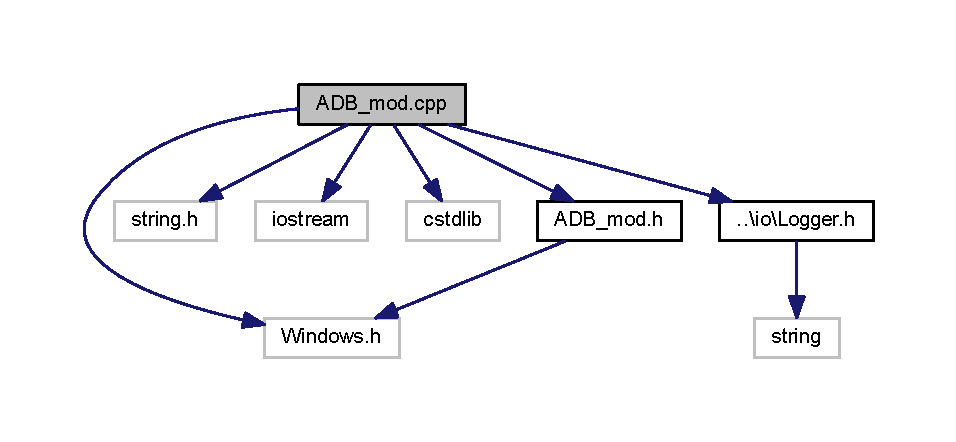
\includegraphics[width=350pt]{_a_d_b__mod_8cpp__incl}
\end{center}
\end{figure}
\subsection*{Функции}
\begin{DoxyCompactItemize}
\item 
void \hyperlink{_a_d_b__mod_8cpp_a5d0a3a01ef690bcd93495becd3273063}{adb} (L\+P\+S\+TR cmd\+Args)
\item 
void \hyperlink{_a_d_b__mod_8cpp_a3b7f80fa75c7705429c3d7402fec0eb0}{fastboot} (L\+P\+S\+TR cmd\+Args)
\item 
void \hyperlink{_a_d_b__mod_8cpp_ad1f1e991625b5f039ea46c20d003ed0f}{adb\+\_\+state} ()
\item 
void \hyperlink{_a_d_b__mod_8cpp_a6b830192de1fd9a84e95434750984282}{adb\+\_\+flash} ()
\item 
void \hyperlink{_a_d_b__mod_8cpp_abe46e301720694fb6fcec4868d54f516}{adb\+\_\+root} ()
\end{DoxyCompactItemize}


\subsection{Подробное описание}
Модуль работы с adb. 

\begin{DoxyAuthor}{Автор}
Darlakon 
\end{DoxyAuthor}


\subsection{Функции}
\mbox{\Hypertarget{_a_d_b__mod_8cpp_a5d0a3a01ef690bcd93495becd3273063}\label{_a_d_b__mod_8cpp_a5d0a3a01ef690bcd93495becd3273063}} 
\index{A\+D\+B\+\_\+mod.\+cpp@{A\+D\+B\+\_\+mod.\+cpp}!adb@{adb}}
\index{adb@{adb}!A\+D\+B\+\_\+mod.\+cpp@{A\+D\+B\+\_\+mod.\+cpp}}
\subsubsection{\texorpdfstring{adb()}{adb()}}
{\footnotesize\ttfamily void adb (\begin{DoxyParamCaption}\item[{L\+P\+S\+TR}]{cmd\+Args }\end{DoxyParamCaption})}

Вызов adb-\/интерфейса. 
\begin{DoxyParams}[1]{Аргументы}
\mbox{\tt in}  & {\em cmd\+Args} & -\/ команда для adb вида \char`\"{}adb X\char`\"{}. \\
\hline
\end{DoxyParams}


См. определение в файле A\+D\+B\+\_\+mod.\+cpp строка 19

\mbox{\Hypertarget{_a_d_b__mod_8cpp_a6b830192de1fd9a84e95434750984282}\label{_a_d_b__mod_8cpp_a6b830192de1fd9a84e95434750984282}} 
\index{A\+D\+B\+\_\+mod.\+cpp@{A\+D\+B\+\_\+mod.\+cpp}!adb\+\_\+flash@{adb\+\_\+flash}}
\index{adb\+\_\+flash@{adb\+\_\+flash}!A\+D\+B\+\_\+mod.\+cpp@{A\+D\+B\+\_\+mod.\+cpp}}
\subsubsection{\texorpdfstring{adb\+\_\+flash()}{adb\_flash()}}
{\footnotesize\ttfamily void adb\+\_\+flash (\begin{DoxyParamCaption}{ }\end{DoxyParamCaption})}

Вызов модуля установки кастомной рекавери. 

См. определение в файле A\+D\+B\+\_\+mod.\+cpp строка 80

\mbox{\Hypertarget{_a_d_b__mod_8cpp_abe46e301720694fb6fcec4868d54f516}\label{_a_d_b__mod_8cpp_abe46e301720694fb6fcec4868d54f516}} 
\index{A\+D\+B\+\_\+mod.\+cpp@{A\+D\+B\+\_\+mod.\+cpp}!adb\+\_\+root@{adb\+\_\+root}}
\index{adb\+\_\+root@{adb\+\_\+root}!A\+D\+B\+\_\+mod.\+cpp@{A\+D\+B\+\_\+mod.\+cpp}}
\subsubsection{\texorpdfstring{adb\+\_\+root()}{adb\_root()}}
{\footnotesize\ttfamily void adb\+\_\+root (\begin{DoxyParamCaption}{ }\end{DoxyParamCaption})}

Вызов модуля получения root-\/прав. 

См. определение в файле A\+D\+B\+\_\+mod.\+cpp строка 107

\mbox{\Hypertarget{_a_d_b__mod_8cpp_ad1f1e991625b5f039ea46c20d003ed0f}\label{_a_d_b__mod_8cpp_ad1f1e991625b5f039ea46c20d003ed0f}} 
\index{A\+D\+B\+\_\+mod.\+cpp@{A\+D\+B\+\_\+mod.\+cpp}!adb\+\_\+state@{adb\+\_\+state}}
\index{adb\+\_\+state@{adb\+\_\+state}!A\+D\+B\+\_\+mod.\+cpp@{A\+D\+B\+\_\+mod.\+cpp}}
\subsubsection{\texorpdfstring{adb\+\_\+state()}{adb\_state()}}
{\footnotesize\ttfamily void adb\+\_\+state (\begin{DoxyParamCaption}{ }\end{DoxyParamCaption})}

Вызов модуля проверки состояния устройства. 

См. определение в файле A\+D\+B\+\_\+mod.\+cpp строка 67

\mbox{\Hypertarget{_a_d_b__mod_8cpp_a3b7f80fa75c7705429c3d7402fec0eb0}\label{_a_d_b__mod_8cpp_a3b7f80fa75c7705429c3d7402fec0eb0}} 
\index{A\+D\+B\+\_\+mod.\+cpp@{A\+D\+B\+\_\+mod.\+cpp}!fastboot@{fastboot}}
\index{fastboot@{fastboot}!A\+D\+B\+\_\+mod.\+cpp@{A\+D\+B\+\_\+mod.\+cpp}}
\subsubsection{\texorpdfstring{fastboot()}{fastboot()}}
{\footnotesize\ttfamily void fastboot (\begin{DoxyParamCaption}\item[{L\+P\+S\+TR}]{cmd\+Args }\end{DoxyParamCaption})}

Вызов fastboot-\/интерфейса. 
\begin{DoxyParams}[1]{Аргументы}
\mbox{\tt in}  & {\em cmd\+Args} & -\/ команда для fastboot вида \char`\"{}fastboot X\char`\"{}. \\
\hline
\end{DoxyParams}


См. определение в файле A\+D\+B\+\_\+mod.\+cpp строка 43


\hypertarget{_a_d_b__mod_8h}{}\section{Файл A\+D\+B\+\_\+mod.\+h}
\label{_a_d_b__mod_8h}\index{A\+D\+B\+\_\+mod.\+h@{A\+D\+B\+\_\+mod.\+h}}


Заголовочный файл с подключением модуля работы с adb.  


{\ttfamily \#include $<$Windows.\+h$>$}\newline
Граф включаемых заголовочных файлов для A\+D\+B\+\_\+mod.\+h\+:
\nopagebreak
\begin{figure}[H]
\begin{center}
\leavevmode
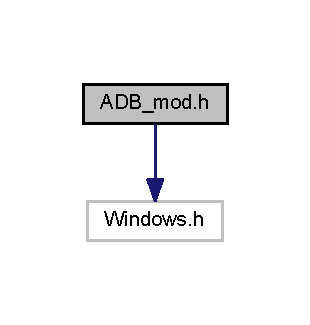
\includegraphics[width=149pt]{_a_d_b__mod_8h__incl}
\end{center}
\end{figure}
Граф файлов, в которые включается этот файл\+:
\nopagebreak
\begin{figure}[H]
\begin{center}
\leavevmode
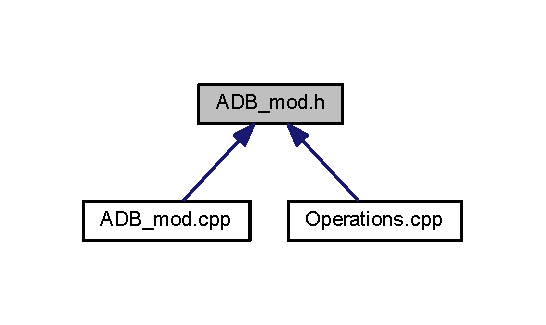
\includegraphics[width=262pt]{_a_d_b__mod_8h__dep__incl}
\end{center}
\end{figure}
\subsection*{Функции}
\begin{DoxyCompactItemize}
\item 
void \hyperlink{_a_d_b__mod_8h_a5d0a3a01ef690bcd93495becd3273063}{adb} (L\+P\+S\+TR cmd\+Args)
\item 
void \hyperlink{_a_d_b__mod_8h_a3b7f80fa75c7705429c3d7402fec0eb0}{fastboot} (L\+P\+S\+TR cmd\+Args)
\item 
void \hyperlink{_a_d_b__mod_8h_ad1f1e991625b5f039ea46c20d003ed0f}{adb\+\_\+state} ()
\item 
void \hyperlink{_a_d_b__mod_8h_a6b830192de1fd9a84e95434750984282}{adb\+\_\+flash} ()
\item 
void \hyperlink{_a_d_b__mod_8h_abe46e301720694fb6fcec4868d54f516}{adb\+\_\+root} ()
\end{DoxyCompactItemize}


\subsection{Подробное описание}
Заголовочный файл с подключением модуля работы с adb. 

\begin{DoxyAuthor}{Автор}
Darlakon 
\end{DoxyAuthor}


\subsection{Функции}
\mbox{\Hypertarget{_a_d_b__mod_8h_a5d0a3a01ef690bcd93495becd3273063}\label{_a_d_b__mod_8h_a5d0a3a01ef690bcd93495becd3273063}} 
\index{A\+D\+B\+\_\+mod.\+h@{A\+D\+B\+\_\+mod.\+h}!adb@{adb}}
\index{adb@{adb}!A\+D\+B\+\_\+mod.\+h@{A\+D\+B\+\_\+mod.\+h}}
\subsubsection{\texorpdfstring{adb()}{adb()}}
{\footnotesize\ttfamily void adb (\begin{DoxyParamCaption}\item[{L\+P\+S\+TR}]{cmd\+Args }\end{DoxyParamCaption})}

Вызов adb-\/интерфейса. 
\begin{DoxyParams}[1]{Аргументы}
\mbox{\tt in}  & {\em cmd\+Args} & -\/ команда для adb вида \char`\"{}adb X\char`\"{}. \\
\hline
\end{DoxyParams}


См. определение в файле A\+D\+B\+\_\+mod.\+cpp строка 19

\mbox{\Hypertarget{_a_d_b__mod_8h_a6b830192de1fd9a84e95434750984282}\label{_a_d_b__mod_8h_a6b830192de1fd9a84e95434750984282}} 
\index{A\+D\+B\+\_\+mod.\+h@{A\+D\+B\+\_\+mod.\+h}!adb\+\_\+flash@{adb\+\_\+flash}}
\index{adb\+\_\+flash@{adb\+\_\+flash}!A\+D\+B\+\_\+mod.\+h@{A\+D\+B\+\_\+mod.\+h}}
\subsubsection{\texorpdfstring{adb\+\_\+flash()}{adb\_flash()}}
{\footnotesize\ttfamily void adb\+\_\+flash (\begin{DoxyParamCaption}{ }\end{DoxyParamCaption})}

Вызов модуля установки кастомной рекавери. 

См. определение в файле A\+D\+B\+\_\+mod.\+cpp строка 80

\mbox{\Hypertarget{_a_d_b__mod_8h_abe46e301720694fb6fcec4868d54f516}\label{_a_d_b__mod_8h_abe46e301720694fb6fcec4868d54f516}} 
\index{A\+D\+B\+\_\+mod.\+h@{A\+D\+B\+\_\+mod.\+h}!adb\+\_\+root@{adb\+\_\+root}}
\index{adb\+\_\+root@{adb\+\_\+root}!A\+D\+B\+\_\+mod.\+h@{A\+D\+B\+\_\+mod.\+h}}
\subsubsection{\texorpdfstring{adb\+\_\+root()}{adb\_root()}}
{\footnotesize\ttfamily void adb\+\_\+root (\begin{DoxyParamCaption}{ }\end{DoxyParamCaption})}

Вызов модуля получения root-\/прав. 

См. определение в файле A\+D\+B\+\_\+mod.\+cpp строка 107

\mbox{\Hypertarget{_a_d_b__mod_8h_ad1f1e991625b5f039ea46c20d003ed0f}\label{_a_d_b__mod_8h_ad1f1e991625b5f039ea46c20d003ed0f}} 
\index{A\+D\+B\+\_\+mod.\+h@{A\+D\+B\+\_\+mod.\+h}!adb\+\_\+state@{adb\+\_\+state}}
\index{adb\+\_\+state@{adb\+\_\+state}!A\+D\+B\+\_\+mod.\+h@{A\+D\+B\+\_\+mod.\+h}}
\subsubsection{\texorpdfstring{adb\+\_\+state()}{adb\_state()}}
{\footnotesize\ttfamily void adb\+\_\+state (\begin{DoxyParamCaption}{ }\end{DoxyParamCaption})}

Вызов модуля проверки состояния устройства. 

См. определение в файле A\+D\+B\+\_\+mod.\+cpp строка 67

\mbox{\Hypertarget{_a_d_b__mod_8h_a3b7f80fa75c7705429c3d7402fec0eb0}\label{_a_d_b__mod_8h_a3b7f80fa75c7705429c3d7402fec0eb0}} 
\index{A\+D\+B\+\_\+mod.\+h@{A\+D\+B\+\_\+mod.\+h}!fastboot@{fastboot}}
\index{fastboot@{fastboot}!A\+D\+B\+\_\+mod.\+h@{A\+D\+B\+\_\+mod.\+h}}
\subsubsection{\texorpdfstring{fastboot()}{fastboot()}}
{\footnotesize\ttfamily void fastboot (\begin{DoxyParamCaption}\item[{L\+P\+S\+TR}]{cmd\+Args }\end{DoxyParamCaption})}

Вызов fastboot-\/интерфейса. 
\begin{DoxyParams}[1]{Аргументы}
\mbox{\tt in}  & {\em cmd\+Args} & -\/ команда для fastboot вида \char`\"{}fastboot X\char`\"{}. \\
\hline
\end{DoxyParams}


См. определение в файле A\+D\+B\+\_\+mod.\+cpp строка 43


\hypertarget{_color_8cpp}{}\section{Файл Color.\+cpp}
\label{_color_8cpp}\index{Color.\+cpp@{Color.\+cpp}}


Модуль работы с цветом в консоли.  


{\ttfamily \#include $<$windows.\+h$>$}\newline
{\ttfamily \#include $<$iostream$>$}\newline
{\ttfamily \#include \char`\"{}Color.\+h\char`\"{}}\newline
Граф включаемых заголовочных файлов для Color.\+cpp\+:
\nopagebreak
\begin{figure}[H]
\begin{center}
\leavevmode
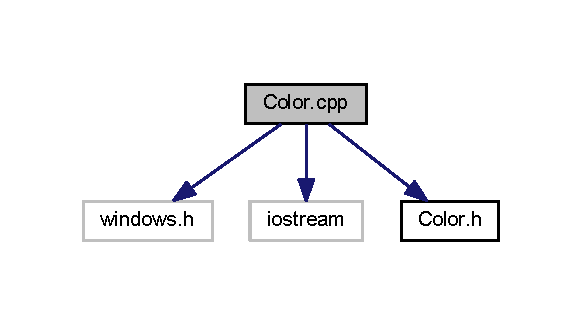
\includegraphics[width=280pt]{_color_8cpp__incl}
\end{center}
\end{figure}
\subsection*{Функции}
\begin{DoxyCompactItemize}
\item 
void \hyperlink{_color_8cpp_a8bfe4542d1f10bae3f4ff0ec688aa67f}{v\+\_\+set\+\_\+color} (\hyperlink{_color_8h_a37dbdc30935031c05304482e1be89d8f}{color} Console\+Text, \hyperlink{_color_8h_a37dbdc30935031c05304482e1be89d8f}{color} Console\+Background)
\item 
void \hyperlink{_color_8cpp_ac4b485399ce8f366e640bbfe8ea40f7b}{v\+\_\+set\+\_\+color} (\hyperlink{_color_8h_a37dbdc30935031c05304482e1be89d8f}{color} Console\+Text)
\item 
void \hyperlink{_color_8cpp_a85ab2b1666a933ebb14c6ffb2db6d4a6}{v\+\_\+color\+\_\+reset} ()
\end{DoxyCompactItemize}


\subsection{Подробное описание}
Модуль работы с цветом в консоли. 

Модуль позволяет менять цвет текста и цвет фона в консоли. 

\subsection{Функции}
\mbox{\Hypertarget{_color_8cpp_a85ab2b1666a933ebb14c6ffb2db6d4a6}\label{_color_8cpp_a85ab2b1666a933ebb14c6ffb2db6d4a6}} 
\index{Color.\+cpp@{Color.\+cpp}!v\+\_\+color\+\_\+reset@{v\+\_\+color\+\_\+reset}}
\index{v\+\_\+color\+\_\+reset@{v\+\_\+color\+\_\+reset}!Color.\+cpp@{Color.\+cpp}}
\subsubsection{\texorpdfstring{v\+\_\+color\+\_\+reset()}{v\_color\_reset()}}
{\footnotesize\ttfamily void v\+\_\+color\+\_\+reset (\begin{DoxyParamCaption}{ }\end{DoxyParamCaption})}

Вернуть цвет текста и цвет заднего фона в консоли к стандартным значениям. 

См. определение в файле Color.\+cpp строка 35

\mbox{\Hypertarget{_color_8cpp_a8bfe4542d1f10bae3f4ff0ec688aa67f}\label{_color_8cpp_a8bfe4542d1f10bae3f4ff0ec688aa67f}} 
\index{Color.\+cpp@{Color.\+cpp}!v\+\_\+set\+\_\+color@{v\+\_\+set\+\_\+color}}
\index{v\+\_\+set\+\_\+color@{v\+\_\+set\+\_\+color}!Color.\+cpp@{Color.\+cpp}}
\subsubsection{\texorpdfstring{v\+\_\+set\+\_\+color()}{v\_set\_color()}\hspace{0.1cm}{\footnotesize\ttfamily [1/2]}}
{\footnotesize\ttfamily void v\+\_\+set\+\_\+color (\begin{DoxyParamCaption}\item[{\hyperlink{_color_8h_a37dbdc30935031c05304482e1be89d8f}{color}}]{Console\+Text,  }\item[{\hyperlink{_color_8h_a37dbdc30935031c05304482e1be89d8f}{color}}]{Console\+Background }\end{DoxyParamCaption})}

Изменение цвета текста и цвета заднего фона в консоли 
\begin{DoxyParams}[1]{Аргументы}
\mbox{\tt in}  & {\em Console\+Text} & цвет текста \\
\hline
\mbox{\tt in}  & {\em Console\+Background} & цвет заднего фона \\
\hline
\end{DoxyParams}
\begin{Desc}
\item[Примеры\+: ]\par
\hyperlink{color_8cpp-example}{color.\+cpp}.\end{Desc}


См. определение в файле Color.\+cpp строка 21

\mbox{\Hypertarget{_color_8cpp_ac4b485399ce8f366e640bbfe8ea40f7b}\label{_color_8cpp_ac4b485399ce8f366e640bbfe8ea40f7b}} 
\index{Color.\+cpp@{Color.\+cpp}!v\+\_\+set\+\_\+color@{v\+\_\+set\+\_\+color}}
\index{v\+\_\+set\+\_\+color@{v\+\_\+set\+\_\+color}!Color.\+cpp@{Color.\+cpp}}
\subsubsection{\texorpdfstring{v\+\_\+set\+\_\+color()}{v\_set\_color()}\hspace{0.1cm}{\footnotesize\ttfamily [2/2]}}
{\footnotesize\ttfamily void v\+\_\+set\+\_\+color (\begin{DoxyParamCaption}\item[{\hyperlink{_color_8h_a37dbdc30935031c05304482e1be89d8f}{color}}]{Console\+Text }\end{DoxyParamCaption})}

Изменение цвета текста в консоли. Задний фон по умолчанию чёрный. 
\begin{DoxyParams}[1]{Аргументы}
\mbox{\tt in}  & {\em Console\+Text} & цвет текста \\
\hline
\end{DoxyParams}


См. определение в файле Color.\+cpp строка 29


\hypertarget{_color_8h}{}\section{Файл Color.\+h}
\label{_color_8h}\index{Color.\+h@{Color.\+h}}


Заголовочный файл с цветами и модулем смены цвета в консоли.  


Граф файлов, в которые включается этот файл\+:
\nopagebreak
\begin{figure}[H]
\begin{center}
\leavevmode
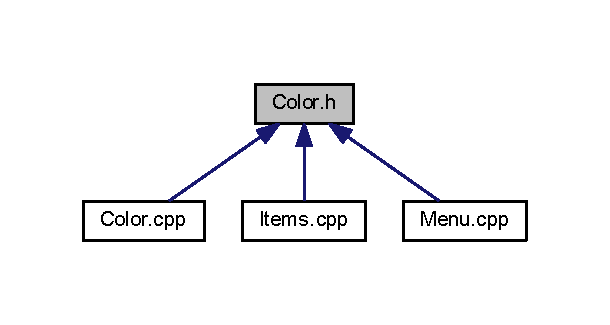
\includegraphics[width=293pt]{_color_8h__dep__incl}
\end{center}
\end{figure}
\subsection*{Перечисления}
\begin{DoxyCompactItemize}
\item 
enum \hyperlink{_color_8h_a37dbdc30935031c05304482e1be89d8f}{color} \{ \newline
\hyperlink{_color_8h_a37dbdc30935031c05304482e1be89d8faf77fb67151d0c18d397069ad8c271ba3}{B\+L\+A\+CK} = 0, 
\hyperlink{_color_8h_a37dbdc30935031c05304482e1be89d8fa35d6719cb4d7577c031b3d79057a1b79}{B\+L\+UE} = 1, 
\hyperlink{_color_8h_a37dbdc30935031c05304482e1be89d8faa60bd322f93178d68184e30e162571ca}{G\+R\+E\+EN} = 2, 
\hyperlink{_color_8h_a37dbdc30935031c05304482e1be89d8faafe71cad474c15ce63b300c470eef8cc}{C\+Y\+AN} = 3, 
\newline
\hyperlink{_color_8h_a37dbdc30935031c05304482e1be89d8faf80f9a890089d211842d59625e561f88}{R\+ED} = 4, 
\hyperlink{_color_8h_a37dbdc30935031c05304482e1be89d8fa56926c820ad72d0977e7ee44d9916e62}{M\+A\+G\+E\+N\+TA} = 5, 
\hyperlink{_color_8h_a37dbdc30935031c05304482e1be89d8fa1fa14482e7e4dc1332ab8c9d995fe570}{B\+R\+O\+WN} = 6, 
\hyperlink{_color_8h_a37dbdc30935031c05304482e1be89d8fa3dcbd50f6d434719ddfb9da673977307}{L\+I\+G\+H\+T\+G\+R\+AY} = 7, 
\newline
\hyperlink{_color_8h_a37dbdc30935031c05304482e1be89d8fa52a9af0edd45f66d37996edcb1ca69f0}{D\+A\+R\+K\+G\+R\+AY} = 8, 
\hyperlink{_color_8h_a37dbdc30935031c05304482e1be89d8fa272b71e84bc2640b193e9fe3c72cb3de}{L\+I\+G\+H\+T\+B\+L\+UE} = 9, 
\hyperlink{_color_8h_a37dbdc30935031c05304482e1be89d8fa0c9ed06b5de60ddd26bb2808e5f4b5dd}{L\+I\+G\+H\+T\+G\+R\+E\+EN} = 10, 
\hyperlink{_color_8h_a37dbdc30935031c05304482e1be89d8fac8d7b8737ca95d137a05f3bb8f3d1a17}{L\+I\+G\+H\+T\+C\+Y\+AN} = 11, 
\newline
\hyperlink{_color_8h_a37dbdc30935031c05304482e1be89d8faf3a6d81d1da6f2134cc3cca6f02b1114}{L\+I\+G\+H\+T\+R\+ED} = 12, 
\hyperlink{_color_8h_a37dbdc30935031c05304482e1be89d8fae19b6d1fedca830c608811b77bd0affc}{L\+I\+G\+H\+T\+M\+A\+G\+E\+N\+TA} = 13, 
\hyperlink{_color_8h_a37dbdc30935031c05304482e1be89d8fa83b21f0c4fad21a5b08f2fa1e1856ca9}{L\+I\+G\+H\+T\+Y\+E\+L\+L\+OW} = 14, 
\hyperlink{_color_8h_a37dbdc30935031c05304482e1be89d8fa283fc479650da98250635b9c3c0e7e50}{W\+H\+I\+TE} = 15
 \}
\end{DoxyCompactItemize}
\subsection*{Функции}
\begin{DoxyCompactItemize}
\item 
void \hyperlink{_color_8h_a8bfe4542d1f10bae3f4ff0ec688aa67f}{v\+\_\+set\+\_\+color} (\hyperlink{_color_8h_a37dbdc30935031c05304482e1be89d8f}{color} Console\+Text, \hyperlink{_color_8h_a37dbdc30935031c05304482e1be89d8f}{color} Console\+Background)
\item 
void \hyperlink{_color_8h_ac4b485399ce8f366e640bbfe8ea40f7b}{v\+\_\+set\+\_\+color} (\hyperlink{_color_8h_a37dbdc30935031c05304482e1be89d8f}{color} Console\+Text)
\item 
void \hyperlink{_color_8h_a85ab2b1666a933ebb14c6ffb2db6d4a6}{v\+\_\+color\+\_\+reset} ()
\end{DoxyCompactItemize}


\subsection{Подробное описание}
Заголовочный файл с цветами и модулем смены цвета в консоли. 

\begin{DoxyAuthor}{Автор}
Sava\+Lione 
\end{DoxyAuthor}


\subsection{Перечисления}
\mbox{\Hypertarget{_color_8h_a37dbdc30935031c05304482e1be89d8f}\label{_color_8h_a37dbdc30935031c05304482e1be89d8f}} 
\index{Color.\+h@{Color.\+h}!color@{color}}
\index{color@{color}!Color.\+h@{Color.\+h}}
\subsubsection{\texorpdfstring{color}{color}}
{\footnotesize\ttfamily enum \hyperlink{_color_8h_a37dbdc30935031c05304482e1be89d8f}{color}}

Цвета \begin{DoxyEnumFields}{Элементы перечислений}
\raisebox{\heightof{T}}[0pt][0pt]{\index{B\+L\+A\+CK@{B\+L\+A\+CK}!Color.\+h@{Color.\+h}}\index{Color.\+h@{Color.\+h}!B\+L\+A\+CK@{B\+L\+A\+CK}}}\mbox{\Hypertarget{_color_8h_a37dbdc30935031c05304482e1be89d8faf77fb67151d0c18d397069ad8c271ba3}\label{_color_8h_a37dbdc30935031c05304482e1be89d8faf77fb67151d0c18d397069ad8c271ba3}} 
B\+L\+A\+CK&Чёрный цвет. \\
\hline

\raisebox{\heightof{T}}[0pt][0pt]{\index{B\+L\+UE@{B\+L\+UE}!Color.\+h@{Color.\+h}}\index{Color.\+h@{Color.\+h}!B\+L\+UE@{B\+L\+UE}}}\mbox{\Hypertarget{_color_8h_a37dbdc30935031c05304482e1be89d8fa35d6719cb4d7577c031b3d79057a1b79}\label{_color_8h_a37dbdc30935031c05304482e1be89d8fa35d6719cb4d7577c031b3d79057a1b79}} 
B\+L\+UE&Синий цвет. \\
\hline

\raisebox{\heightof{T}}[0pt][0pt]{\index{G\+R\+E\+EN@{G\+R\+E\+EN}!Color.\+h@{Color.\+h}}\index{Color.\+h@{Color.\+h}!G\+R\+E\+EN@{G\+R\+E\+EN}}}\mbox{\Hypertarget{_color_8h_a37dbdc30935031c05304482e1be89d8faa60bd322f93178d68184e30e162571ca}\label{_color_8h_a37dbdc30935031c05304482e1be89d8faa60bd322f93178d68184e30e162571ca}} 
G\+R\+E\+EN&Зелёный цвет. \\
\hline

\raisebox{\heightof{T}}[0pt][0pt]{\index{C\+Y\+AN@{C\+Y\+AN}!Color.\+h@{Color.\+h}}\index{Color.\+h@{Color.\+h}!C\+Y\+AN@{C\+Y\+AN}}}\mbox{\Hypertarget{_color_8h_a37dbdc30935031c05304482e1be89d8faafe71cad474c15ce63b300c470eef8cc}\label{_color_8h_a37dbdc30935031c05304482e1be89d8faafe71cad474c15ce63b300c470eef8cc}} 
C\+Y\+AN&Сине-\/зелёный цвет. \\
\hline

\raisebox{\heightof{T}}[0pt][0pt]{\index{R\+ED@{R\+ED}!Color.\+h@{Color.\+h}}\index{Color.\+h@{Color.\+h}!R\+ED@{R\+ED}}}\mbox{\Hypertarget{_color_8h_a37dbdc30935031c05304482e1be89d8faf80f9a890089d211842d59625e561f88}\label{_color_8h_a37dbdc30935031c05304482e1be89d8faf80f9a890089d211842d59625e561f88}} 
R\+ED&Красный цвет. \\
\hline

\raisebox{\heightof{T}}[0pt][0pt]{\index{M\+A\+G\+E\+N\+TA@{M\+A\+G\+E\+N\+TA}!Color.\+h@{Color.\+h}}\index{Color.\+h@{Color.\+h}!M\+A\+G\+E\+N\+TA@{M\+A\+G\+E\+N\+TA}}}\mbox{\Hypertarget{_color_8h_a37dbdc30935031c05304482e1be89d8fa56926c820ad72d0977e7ee44d9916e62}\label{_color_8h_a37dbdc30935031c05304482e1be89d8fa56926c820ad72d0977e7ee44d9916e62}} 
M\+A\+G\+E\+N\+TA&Пурпурный цвет. \\
\hline

\raisebox{\heightof{T}}[0pt][0pt]{\index{B\+R\+O\+WN@{B\+R\+O\+WN}!Color.\+h@{Color.\+h}}\index{Color.\+h@{Color.\+h}!B\+R\+O\+WN@{B\+R\+O\+WN}}}\mbox{\Hypertarget{_color_8h_a37dbdc30935031c05304482e1be89d8fa1fa14482e7e4dc1332ab8c9d995fe570}\label{_color_8h_a37dbdc30935031c05304482e1be89d8fa1fa14482e7e4dc1332ab8c9d995fe570}} 
B\+R\+O\+WN&Коричневый цвет. \\
\hline

\raisebox{\heightof{T}}[0pt][0pt]{\index{L\+I\+G\+H\+T\+G\+R\+AY@{L\+I\+G\+H\+T\+G\+R\+AY}!Color.\+h@{Color.\+h}}\index{Color.\+h@{Color.\+h}!L\+I\+G\+H\+T\+G\+R\+AY@{L\+I\+G\+H\+T\+G\+R\+AY}}}\mbox{\Hypertarget{_color_8h_a37dbdc30935031c05304482e1be89d8fa3dcbd50f6d434719ddfb9da673977307}\label{_color_8h_a37dbdc30935031c05304482e1be89d8fa3dcbd50f6d434719ddfb9da673977307}} 
L\+I\+G\+H\+T\+G\+R\+AY&Светло-\/серый цвет. \\
\hline

\raisebox{\heightof{T}}[0pt][0pt]{\index{D\+A\+R\+K\+G\+R\+AY@{D\+A\+R\+K\+G\+R\+AY}!Color.\+h@{Color.\+h}}\index{Color.\+h@{Color.\+h}!D\+A\+R\+K\+G\+R\+AY@{D\+A\+R\+K\+G\+R\+AY}}}\mbox{\Hypertarget{_color_8h_a37dbdc30935031c05304482e1be89d8fa52a9af0edd45f66d37996edcb1ca69f0}\label{_color_8h_a37dbdc30935031c05304482e1be89d8fa52a9af0edd45f66d37996edcb1ca69f0}} 
D\+A\+R\+K\+G\+R\+AY&Тёмно-\/серый цвет. \\
\hline

\raisebox{\heightof{T}}[0pt][0pt]{\index{L\+I\+G\+H\+T\+B\+L\+UE@{L\+I\+G\+H\+T\+B\+L\+UE}!Color.\+h@{Color.\+h}}\index{Color.\+h@{Color.\+h}!L\+I\+G\+H\+T\+B\+L\+UE@{L\+I\+G\+H\+T\+B\+L\+UE}}}\mbox{\Hypertarget{_color_8h_a37dbdc30935031c05304482e1be89d8fa272b71e84bc2640b193e9fe3c72cb3de}\label{_color_8h_a37dbdc30935031c05304482e1be89d8fa272b71e84bc2640b193e9fe3c72cb3de}} 
L\+I\+G\+H\+T\+B\+L\+UE&Светло-\/синий цвет. \\
\hline

\raisebox{\heightof{T}}[0pt][0pt]{\index{L\+I\+G\+H\+T\+G\+R\+E\+EN@{L\+I\+G\+H\+T\+G\+R\+E\+EN}!Color.\+h@{Color.\+h}}\index{Color.\+h@{Color.\+h}!L\+I\+G\+H\+T\+G\+R\+E\+EN@{L\+I\+G\+H\+T\+G\+R\+E\+EN}}}\mbox{\Hypertarget{_color_8h_a37dbdc30935031c05304482e1be89d8fa0c9ed06b5de60ddd26bb2808e5f4b5dd}\label{_color_8h_a37dbdc30935031c05304482e1be89d8fa0c9ed06b5de60ddd26bb2808e5f4b5dd}} 
L\+I\+G\+H\+T\+G\+R\+E\+EN&Светло-\/зелёный цвет. \\
\hline

\raisebox{\heightof{T}}[0pt][0pt]{\index{L\+I\+G\+H\+T\+C\+Y\+AN@{L\+I\+G\+H\+T\+C\+Y\+AN}!Color.\+h@{Color.\+h}}\index{Color.\+h@{Color.\+h}!L\+I\+G\+H\+T\+C\+Y\+AN@{L\+I\+G\+H\+T\+C\+Y\+AN}}}\mbox{\Hypertarget{_color_8h_a37dbdc30935031c05304482e1be89d8fac8d7b8737ca95d137a05f3bb8f3d1a17}\label{_color_8h_a37dbdc30935031c05304482e1be89d8fac8d7b8737ca95d137a05f3bb8f3d1a17}} 
L\+I\+G\+H\+T\+C\+Y\+AN&Светло-\/сине-\/зелёный цвет. \\
\hline

\raisebox{\heightof{T}}[0pt][0pt]{\index{L\+I\+G\+H\+T\+R\+ED@{L\+I\+G\+H\+T\+R\+ED}!Color.\+h@{Color.\+h}}\index{Color.\+h@{Color.\+h}!L\+I\+G\+H\+T\+R\+ED@{L\+I\+G\+H\+T\+R\+ED}}}\mbox{\Hypertarget{_color_8h_a37dbdc30935031c05304482e1be89d8faf3a6d81d1da6f2134cc3cca6f02b1114}\label{_color_8h_a37dbdc30935031c05304482e1be89d8faf3a6d81d1da6f2134cc3cca6f02b1114}} 
L\+I\+G\+H\+T\+R\+ED&Светло-\/красный цвет. \\
\hline

\raisebox{\heightof{T}}[0pt][0pt]{\index{L\+I\+G\+H\+T\+M\+A\+G\+E\+N\+TA@{L\+I\+G\+H\+T\+M\+A\+G\+E\+N\+TA}!Color.\+h@{Color.\+h}}\index{Color.\+h@{Color.\+h}!L\+I\+G\+H\+T\+M\+A\+G\+E\+N\+TA@{L\+I\+G\+H\+T\+M\+A\+G\+E\+N\+TA}}}\mbox{\Hypertarget{_color_8h_a37dbdc30935031c05304482e1be89d8fae19b6d1fedca830c608811b77bd0affc}\label{_color_8h_a37dbdc30935031c05304482e1be89d8fae19b6d1fedca830c608811b77bd0affc}} 
L\+I\+G\+H\+T\+M\+A\+G\+E\+N\+TA&Светло-\/пурпурный цвет. \\
\hline

\raisebox{\heightof{T}}[0pt][0pt]{\index{L\+I\+G\+H\+T\+Y\+E\+L\+L\+OW@{L\+I\+G\+H\+T\+Y\+E\+L\+L\+OW}!Color.\+h@{Color.\+h}}\index{Color.\+h@{Color.\+h}!L\+I\+G\+H\+T\+Y\+E\+L\+L\+OW@{L\+I\+G\+H\+T\+Y\+E\+L\+L\+OW}}}\mbox{\Hypertarget{_color_8h_a37dbdc30935031c05304482e1be89d8fa83b21f0c4fad21a5b08f2fa1e1856ca9}\label{_color_8h_a37dbdc30935031c05304482e1be89d8fa83b21f0c4fad21a5b08f2fa1e1856ca9}} 
L\+I\+G\+H\+T\+Y\+E\+L\+L\+OW&Светло-\/жёлтый цвет. \\
\hline

\raisebox{\heightof{T}}[0pt][0pt]{\index{W\+H\+I\+TE@{W\+H\+I\+TE}!Color.\+h@{Color.\+h}}\index{Color.\+h@{Color.\+h}!W\+H\+I\+TE@{W\+H\+I\+TE}}}\mbox{\Hypertarget{_color_8h_a37dbdc30935031c05304482e1be89d8fa283fc479650da98250635b9c3c0e7e50}\label{_color_8h_a37dbdc30935031c05304482e1be89d8fa283fc479650da98250635b9c3c0e7e50}} 
W\+H\+I\+TE&Белый цвет. \\
\hline

\end{DoxyEnumFields}


См. определение в файле Color.\+h строка 9



\subsection{Функции}
\mbox{\Hypertarget{_color_8h_a85ab2b1666a933ebb14c6ffb2db6d4a6}\label{_color_8h_a85ab2b1666a933ebb14c6ffb2db6d4a6}} 
\index{Color.\+h@{Color.\+h}!v\+\_\+color\+\_\+reset@{v\+\_\+color\+\_\+reset}}
\index{v\+\_\+color\+\_\+reset@{v\+\_\+color\+\_\+reset}!Color.\+h@{Color.\+h}}
\subsubsection{\texorpdfstring{v\+\_\+color\+\_\+reset()}{v\_color\_reset()}}
{\footnotesize\ttfamily void v\+\_\+color\+\_\+reset (\begin{DoxyParamCaption}{ }\end{DoxyParamCaption})}

Вернуть цвет текста и цвет заднего фона в консоли к стандартным значениям. 

См. определение в файле Color.\+cpp строка 35

\mbox{\Hypertarget{_color_8h_a8bfe4542d1f10bae3f4ff0ec688aa67f}\label{_color_8h_a8bfe4542d1f10bae3f4ff0ec688aa67f}} 
\index{Color.\+h@{Color.\+h}!v\+\_\+set\+\_\+color@{v\+\_\+set\+\_\+color}}
\index{v\+\_\+set\+\_\+color@{v\+\_\+set\+\_\+color}!Color.\+h@{Color.\+h}}
\subsubsection{\texorpdfstring{v\+\_\+set\+\_\+color()}{v\_set\_color()}\hspace{0.1cm}{\footnotesize\ttfamily [1/2]}}
{\footnotesize\ttfamily void v\+\_\+set\+\_\+color (\begin{DoxyParamCaption}\item[{\hyperlink{_color_8h_a37dbdc30935031c05304482e1be89d8f}{color}}]{Console\+Text,  }\item[{\hyperlink{_color_8h_a37dbdc30935031c05304482e1be89d8f}{color}}]{Console\+Background }\end{DoxyParamCaption})}

Изменение цвета текста и цвета заднего фона в консоли. 
\begin{DoxyParams}[1]{Аргументы}
\mbox{\tt in}  & {\em Console\+Text} & цвет текста. \\
\hline
\mbox{\tt in}  & {\em Console\+Background} & цвет заднего фона.\\
\hline
\end{DoxyParams}
Изменение цвета текста и цвета заднего фона в консоли 
\begin{DoxyParams}[1]{Аргументы}
\mbox{\tt in}  & {\em Console\+Text} & цвет текста \\
\hline
\mbox{\tt in}  & {\em Console\+Background} & цвет заднего фона \\
\hline
\end{DoxyParams}


См. определение в файле Color.\+cpp строка 21

\mbox{\Hypertarget{_color_8h_ac4b485399ce8f366e640bbfe8ea40f7b}\label{_color_8h_ac4b485399ce8f366e640bbfe8ea40f7b}} 
\index{Color.\+h@{Color.\+h}!v\+\_\+set\+\_\+color@{v\+\_\+set\+\_\+color}}
\index{v\+\_\+set\+\_\+color@{v\+\_\+set\+\_\+color}!Color.\+h@{Color.\+h}}
\subsubsection{\texorpdfstring{v\+\_\+set\+\_\+color()}{v\_set\_color()}\hspace{0.1cm}{\footnotesize\ttfamily [2/2]}}
{\footnotesize\ttfamily void v\+\_\+set\+\_\+color (\begin{DoxyParamCaption}\item[{\hyperlink{_color_8h_a37dbdc30935031c05304482e1be89d8f}{color}}]{Console\+Text }\end{DoxyParamCaption})}

Изменение цвета текста в консоли. Задний фон по умолчанию чёрный. 
\begin{DoxyParams}[1]{Аргументы}
\mbox{\tt in}  & {\em Console\+Text} & цвет текста.\\
\hline
\end{DoxyParams}
Изменение цвета текста в консоли. Задний фон по умолчанию чёрный. 
\begin{DoxyParams}[1]{Аргументы}
\mbox{\tt in}  & {\em Console\+Text} & цвет текста \\
\hline
\end{DoxyParams}


См. определение в файле Color.\+cpp строка 29


\hypertarget{_constants_8h}{}\section{Файл Constants.\+h}
\label{_constants_8h}\index{Constants.\+h@{Constants.\+h}}


Заголовочный файл с константами.  


{\ttfamily \#include $<$string$>$}\newline
Граф включаемых заголовочных файлов для Constants.\+h\+:
\nopagebreak
\begin{figure}[H]
\begin{center}
\leavevmode
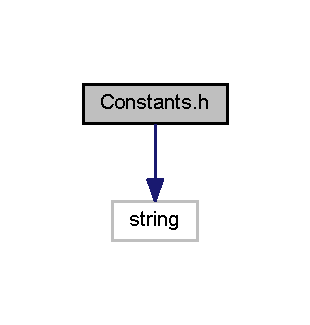
\includegraphics[width=149pt]{_constants_8h__incl}
\end{center}
\end{figure}
Граф файлов, в которые включается этот файл\+:
\nopagebreak
\begin{figure}[H]
\begin{center}
\leavevmode
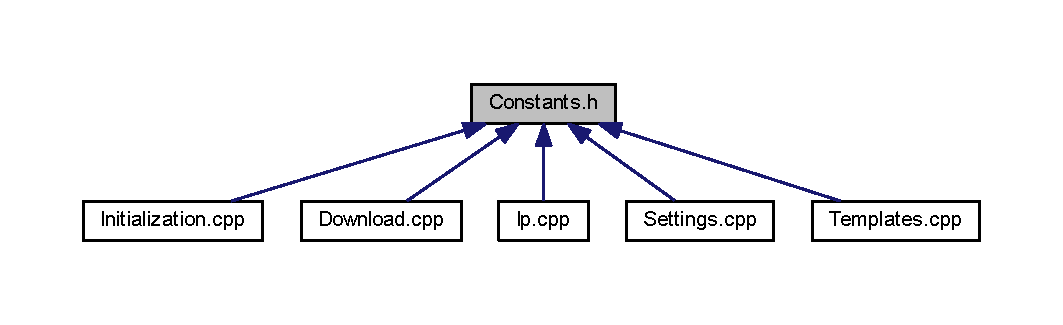
\includegraphics[width=350pt]{_constants_8h__dep__incl}
\end{center}
\end{figure}
\subsection*{Пространства имен}
\begin{DoxyCompactItemize}
\item 
 \hyperlink{namespaceradix}{radix}
\item 
 \hyperlink{namespacemenu}{menu}
\item 
 \hyperlink{namespacelogo}{logo}
\end{DoxyCompactItemize}
\subsection*{Переменные}
\begin{DoxyCompactItemize}
\item 
const size\+\_\+t \hyperlink{namespaceradix_a82e81e89088b6430b7ec11a8a0329e9c}{radix\+::buff\+\_\+size} = 32
\item 
const size\+\_\+t \hyperlink{namespaceradix_a8f000aabf647d34fd877c33958bad711}{radix\+::buff\+\_\+ruleslist} = 256
\item 
const char \hyperlink{namespaceradix_a11c5bfe5c65a0f88a2a950111c6ffc09}{radix\+::logger\+\_\+list} \mbox{[}$\,$\mbox{]} = \char`\"{}logger.\+log\char`\"{}
\item 
const char \hyperlink{namespaceradix_a43bff57dbd1b7dcebee0228ccbab7f17}{radix\+::settings\+\_\+list} \mbox{[}$\,$\mbox{]} = \char`\"{}settings.\+ini\char`\"{}
\item 
const char \hyperlink{namespaceradix_a123392a7ece6e11efaf3ad3df291ff3d}{radix\+::firmware\+\_\+way} \mbox{[}$\,$\mbox{]} = \char`\"{}\textbackslash{}\textbackslash{}assets\textbackslash{}\textbackslash{}firmware\textbackslash{}\textbackslash{}\char`\"{}
\item 
const char \hyperlink{namespaceradix_aa90f63f1d0143b58469670ccbb86cfc4}{radix\+::patch} \mbox{[}$\,$\mbox{]} = \char`\"{}\textbackslash{}\textbackslash{}assets\textbackslash{}\textbackslash{}\char`\"{}
\item 
const char \hyperlink{namespaceradix_a01a09f0b88f6fd375ea20667bd318035}{radix\+::expansion\+\_\+file} \mbox{[}$\,$\mbox{]} = \char`\"{}.zip\char`\"{}
\item 
const char \hyperlink{namespaceradix_a91c21d6be385236a564ef5bf1f3f3602}{radix\+::recovery\+\_\+file} \mbox{[}$\,$\mbox{]} = \char`\"{}recovery.\+img\char`\"{}
\item 
const char \hyperlink{namespaceradix_abcd4cb3ab01a6a642ba224e2d9b1eda5}{radix\+::su\+\_\+file} \mbox{[}$\,$\mbox{]} = \char`\"{}su.\+zip\char`\"{}
\item 
const char \hyperlink{namespaceradix_a9f0187ab8d7f9931ed08159a233408c0}{radix\+::not\+\_\+found} \mbox{[}$\,$\mbox{]} = \char`\"{} not found.\char`\"{}
\item 
const char \hyperlink{namespaceradix_a27726ea7eb8e2bea153425bce9328be5}{radix\+::found} \mbox{[}$\,$\mbox{]} = \char`\"{} found.\char`\"{}
\item 
const char \hyperlink{namespaceradix_ad5e76eca849713be360ed8478545d801}{radix\+::ch\+\_\+user\+\_\+continue} \mbox{[}$\,$\mbox{]} = \char`\"{}The user continued the program despite the error.\char`\"{}
\item 
const char \hyperlink{namespaceradix_afd1855af7805a1bb408ea9175a626ac7}{radix\+::ch\+\_\+user\+\_\+not\+\_\+continue} \mbox{[}$\,$\mbox{]} = \char`\"{}The user did not continue the program despite the error.\char`\"{}
\item 
const std\+::string \hyperlink{namespacemenu_ac0906d6effd5dc68552a724a3edb9330}{menu\+::indentation} = \char`\"{} \char`\"{}
\item 
const std\+::string \hyperlink{namespacemenu_ab9230afa22bdf260e3944290026a5a86}{menu\+::frame\+\_\+left} = \char`\"{} $<$\char`\"{}
\item 
const std\+::string \hyperlink{namespacemenu_a3f786c7ab3caec7dfef9e1fa61b52ae7}{menu\+::frame\+\_\+right} = \char`\"{}$>$ \char`\"{}
\item 
const size\+\_\+t \hyperlink{namespacemenu_aa3bc0d7f62e04dc52dd8f276902448ae}{menu\+::loading\+\_\+size} = 25
\item 
const bool \hyperlink{namespacemenu_aaea5c70964114a416caa58676ddf8066}{menu\+::loading\+\_\+check\+\_\+module} = false
\item 
const size\+\_\+t \hyperlink{namespacemenu_a69bce854c4a150920a5c77eede8cab0a}{menu\+::loading\+\_\+check\+\_\+module\+\_\+sleep} = 1000
\item 
const char \hyperlink{namespacemenu_a56af6a2d586e2b6baa4ebf128a690266}{menu\+::loading\+\_\+left} = \textquotesingle{}\mbox{[}\textquotesingle{}
\item 
const char \hyperlink{namespacemenu_a272b2c0c591457b2aeccaae0c122a1fc}{menu\+::loading\+\_\+right} = \textquotesingle{}\mbox{]}\textquotesingle{}
\item 
const char \hyperlink{namespacemenu_ab79f369195d81dcb241b1ab5269c9d3d}{menu\+::loading\+\_\+progress} = \textquotesingle{}$\vert$\textquotesingle{}
\item 
const char \hyperlink{namespacemenu_ad004c327a8a1c14388a6c7f23d6953a6}{menu\+::loading\+\_\+indenting} = \textquotesingle{} \textquotesingle{}
\item 
const size\+\_\+t \hyperlink{namespacemenu_af10d26be126a6efaa57428f629514f93}{menu\+::backspace} = 8
\item 
const size\+\_\+t \hyperlink{namespacemenu_a9ca2724b99053483cb2af7b49563db95}{menu\+::enter} = 13
\item 
const size\+\_\+t \hyperlink{namespacemenu_a31d13ed09dc59c7220146bd432fc3787}{menu\+::esc} = 27
\item 
const size\+\_\+t \hyperlink{namespacemenu_a480dcaab18029e9e82979360297d9841}{menu\+::space} = 32
\item 
const size\+\_\+t \hyperlink{namespacemenu_a5e6bc193fc3cb9a0cfce7370a1578aeb}{menu\+::arrow\+\_\+up} = 72
\item 
const size\+\_\+t \hyperlink{namespacemenu_a971b85d59fefa12b99efe533fa977e8f}{menu\+::arrow\+\_\+left} = 75
\item 
const size\+\_\+t \hyperlink{namespacemenu_a5ac4dac780ca5b41b206c7ddf5f9905e}{menu\+::arrow\+\_\+right} = 77
\item 
const size\+\_\+t \hyperlink{namespacemenu_a23e79ce5c613d90b85f9a2c064f610f3}{menu\+::arrow\+\_\+down} = 80
\item 
const size\+\_\+t \hyperlink{namespacemenu_af11c563a29975fcfa8a0bac77b2630f7}{menu\+::special} = 224
\item 
const std\+::string \hyperlink{namespacelogo_a75fab9a3dcd27565e40b08dbbcbf5e6b}{logo\+::border} = \char`\"{}===========================\textbackslash{}n\char`\"{}
\item 
const std\+::string \hyperlink{namespacelogo_adf18ab31906b644891fc8311df747a9d}{logo\+::little\+\_\+help} = \char`\"{}==== $<$-\/ use to move -\/$>$ ====\textbackslash{}n\char`\"{}
\item 
const std\+::string \hyperlink{namespacelogo_ae5491adc000fde7d3d8229372c877da2}{logo\+::license} = \char`\"{}Do you agree with the license?\textbackslash{}n\char`\"{}
\item 
const std\+::string \hyperlink{namespacelogo_a7570bf74bf945a06ced26f6fccaeab53}{logo\+::move\+\_\+indentation} = \char`\"{} \char`\"{}
\item 
const std\+::string \hyperlink{namespacelogo_a03b6b80b5648e7dbbbf00b258df733b6}{logo\+::move} = \char`\"{}$<$-\/ use to move -\/$>$\textbackslash{}n\char`\"{}
\item 
const std\+::string \hyperlink{namespacelogo_abbbdbfbbcae50e2017f3ed1bdf0e1fa3}{logo\+::radix} = \char`\"{} \+\_\+\+\_\+\+\_\+\+\_\+\+\_\+ \+\_\+ \+\_\+ \textbackslash{}n $\vert$ \+\_\+\+\_\+ \textbackslash{}\textbackslash{} $\vert$ (\+\_\+) \textbackslash{}n $\vert$ $\vert$\+\_\+\+\_\+) $\vert$\+\_\+\+\_\+ \+\_\+ \+\_\+\+\_\+$\vert$ $\vert$\+\_\+\+\_\+\+\_\+ \+\_\+\+\_\+\textbackslash{}n $\vert$ \+\_\+ // \+\_\+` $\vert$/ \+\_\+` $\vert$ \textbackslash{}\textbackslash{} \textbackslash{}\textbackslash{}/ /\textbackslash{}n $\vert$ $\vert$ \textbackslash{}\textbackslash{} \textbackslash{}\textbackslash{} (\+\_\+$\vert$ $\vert$ (\+\_\+$\vert$ $\vert$ $\vert$$>$ $<$ \textbackslash{}n $\vert$\+\_\+$\vert$ \textbackslash{}\textbackslash{}\+\_\+\textbackslash{}\textbackslash{}\+\_\+\+\_\+,\+\_\+$\vert$\textbackslash{}\textbackslash{}\+\_\+\+\_\+,\+\_\+$\vert$\+\_\+/\+\_\+/\textbackslash{}\textbackslash{}\+\_\+\textbackslash{}\textbackslash{} \textbackslash{}n\char`\"{}
\item 
const std\+::string \hyperlink{namespacelogo_ad29ac81055f7eb3624a283f55af8d5ad}{logo\+::loading} = \char`\"{} \+\_\+ \+\_\+ \textbackslash{}n $\vert$ $\vert$ $\vert$ $\vert$\textbackslash{}n $\vert$ $\vert$ \+\_\+\+\_\+\+\_\+ \+\_\+\+\_\+ \+\_\+ \+\_\+\+\_\+$\vert$ $\vert$\textbackslash{}n $\vert$ $\vert$ / \+\_\+ \textbackslash{}\textbackslash{} / \+\_\+` $\vert$/ \+\_\+` $\vert$\textbackslash{}n $\vert$ $\vert$\+\_\+\+\_\+\+\_\+$\vert$ (\+\_\+) $\vert$ (\+\_\+$\vert$ $\vert$ (\+\_\+$\vert$ $\vert$\textbackslash{}n $\vert$\+\_\+\+\_\+\+\_\+\+\_\+\+\_\+\+\_\+\textbackslash{}\textbackslash{}\+\_\+\+\_\+\+\_\+/ \textbackslash{}\textbackslash{}\+\_\+\+\_\+,\+\_\+$\vert$\textbackslash{}\textbackslash{}\+\_\+\+\_\+,\+\_\+$\vert$\textbackslash{}n\char`\"{}
\item 
const std\+::string \hyperlink{namespacelogo_aba8ca66bcf8abe6a0991a13887671863}{logo\+::exit} = \char`\"{} \+\_\+\+\_\+\+\_\+\+\_\+\+\_\+\+\_\+ \+\_\+ \+\_\+ \textbackslash{}n $\vert$ \+\_\+\+\_\+\+\_\+\+\_\+$\vert$ (\+\_\+) $\vert$ \textbackslash{}n $\vert$ $\vert$\+\_\+\+\_\+ \+\_\+\+\_\+ \+\_\+\+\_\+\+\_\+$\vert$ $\vert$\+\_\+ \textbackslash{}n $\vert$ \+\_\+\+\_\+$\vert$ \textbackslash{}\textbackslash{} \textbackslash{}\textbackslash{}/ / $\vert$ \+\_\+\+\_\+$\vert$\textbackslash{}n $\vert$ $\vert$\+\_\+\+\_\+\+\_\+\+\_\+ $>$ $<$$\vert$ $\vert$ $\vert$\+\_\+ \textbackslash{}n $\vert$\+\_\+\+\_\+\+\_\+\+\_\+\+\_\+\+\_\+/\+\_\+/\textbackslash{}\textbackslash{}\+\_\+\textbackslash{}\textbackslash{}\+\_\+$\vert$\textbackslash{}\textbackslash{}\+\_\+\+\_\+$\vert$\textbackslash{}n\char`\"{}
\item 
const std\+::string \hyperlink{namespacelogo_a6bb2bd19b13072f69598ed9f64b77350}{logo\+::s\+\_\+continue} = \char`\"{}Continue?\textbackslash{}n\char`\"{}
\item 
const std\+::string \hyperlink{namespacelogo_a0a26b9dd91d59364dce6d78c217af1a0}{logo\+::s\+\_\+manual} = \char`\"{} User Manual\textbackslash{}n0) If necessary, install drivers from assets/Drivers\+\_\+\+Universal folder.\textbackslash{}n1) Enable U\+SB debugging on your device.\textbackslash{}n You\textquotesingle{}ll need to become developer by tapping \textbackslash{}\char`\"{}Build Number\textbackslash{}\char`\"{} in \textbackslash{}\char`\"{}About Device\textbackslash{}\char`\"{} section.\textbackslash{}n Then go to Developer section and enable debugging.\textbackslash{}n2) Plug in your device, accept debugging request.\textbackslash{}n3) Put files \textquotesingle{}recovery.\+img\textquotesingle{} and \textquotesingle{}su.\+zip\textquotesingle{} in program directory(next to Radix.\+exe)\textbackslash{}n4) Proceed.\char`\"{}
\item 
const std\+::string \hyperlink{namespacelogo_ac55b3c4624556820a987ccdf67101bae}{logo\+::enter} = \char`\"{}Press any key to continue.\char`\"{}
\item 
const std\+::string \hyperlink{namespacelogo_ae3d10c2b731b19f239a7311af363354c}{logo\+::eula} = \char`\"{}Copyright (c) 2017 Radix\textbackslash{}n\textbackslash{}n\+T\+HE S\+O\+F\+T\+W\+A\+RE IS P\+R\+O\+V\+I\+D\+ED \textbackslash{}\char`\"{}AS I\+S\textbackslash{}\char`\"{}, W\+I\+T\+H\+O\+UT W\+A\+R\+R\+A\+N\+TY OF A\+NY K\+I\+ND, E\+X\+P\+R\+E\+SS OR I\+M\+P\+L\+I\+ED, I\+N\+C\+L\+U\+D\+I\+NG B\+UT N\+OT L\+I\+M\+I\+T\+ED TO T\+HE W\+A\+R\+R\+A\+N\+T\+I\+ES OF M\+E\+R\+C\+H\+A\+N\+T\+A\+B\+I\+L\+I\+TY, F\+I\+T\+N\+E\+SS F\+OR A \textbackslash{}n\+P\+A\+R\+T\+I\+C\+U\+L\+AR P\+U\+R\+P\+O\+SE A\+ND N\+O\+N\+I\+N\+F\+R\+I\+N\+G\+E\+M\+E\+N\+T. IN NO E\+V\+E\+NT S\+H\+A\+LL T\+HE A\+U\+T\+H\+O\+RS OR C\+O\+P\+Y\+R\+I\+G\+HT H\+O\+L\+D\+E\+RS BE L\+I\+A\+B\+LE F\+OR A\+NY C\+L\+A\+IM, D\+A\+M\+A\+G\+ES OR O\+T\+H\+ER L\+I\+A\+B\+I\+L\+I\+TY, W\+H\+E\+T\+H\+ER IN AN \textbackslash{}n\+A\+C\+T\+I\+ON OF C\+O\+N\+T\+R\+A\+CT, T\+O\+RT OR O\+T\+H\+E\+R\+W\+I\+SE, A\+R\+I\+S\+I\+NG F\+R\+OM, O\+UT OF OR IN C\+O\+N\+N\+E\+C\+T\+I\+ON W\+I\+TH T\+HE S\+O\+F\+T\+W\+A\+RE OR T\+HE U\+SE OR O\+T\+H\+ER D\+E\+A\+L\+I\+N\+GS IN T\+HE S\+O\+F\+T\+W\+A\+R\+E.\textbackslash{}n\char`\"{}
\end{DoxyCompactItemize}


\subsection{Подробное описание}
Заголовочный файл с константами. 


\hypertarget{_items_8cpp}{}\section{Файл Items.\+cpp}
\label{_items_8cpp}\index{Items.\+cpp@{Items.\+cpp}}


Создание меню.  


{\ttfamily \#include $<$iostream$>$}\newline
{\ttfamily \#include $<$Windows.\+h$>$}\newline
{\ttfamily \#include \char`\"{}..\textbackslash{}core\textbackslash{}\+Constants.\+h\char`\"{}}\newline
{\ttfamily \#include \char`\"{}..\textbackslash{}core\textbackslash{}\+Color.\+h\char`\"{}}\newline
{\ttfamily \#include \char`\"{}..\textbackslash{}ui\textbackslash{}\+Menu.\+h\char`\"{}}\newline
Граф включаемых заголовочных файлов для Items.\+cpp\+:
\nopagebreak
\begin{figure}[H]
\begin{center}
\leavevmode
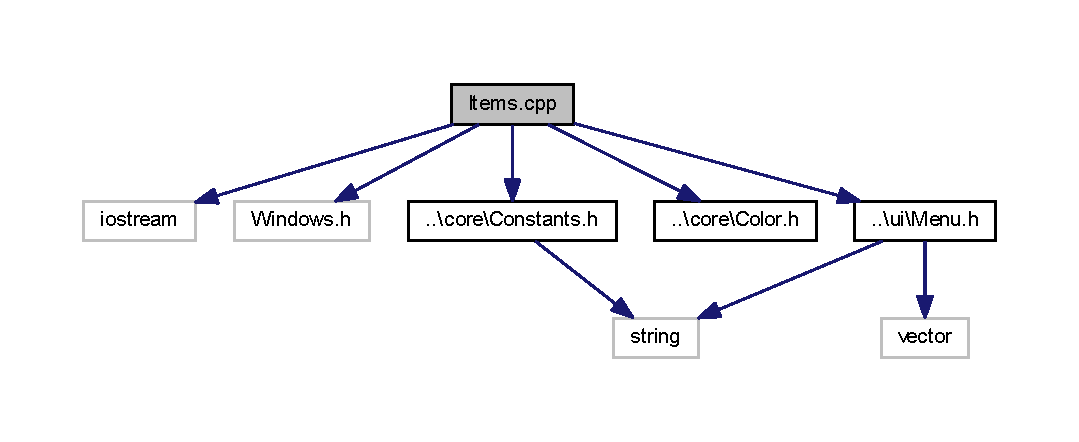
\includegraphics[width=350pt]{_items_8cpp__incl}
\end{center}
\end{figure}
\subsection*{Функции}
\begin{DoxyCompactItemize}
\item 
void \hyperlink{_items_8cpp_ad151996f106cf7ff3fad3914fbf611c5}{v\+\_\+mainmenu\+\_\+before} ()
\begin{DoxyCompactList}\small\item\em Блок до выполнения модуля меню. \end{DoxyCompactList}\item 
void \hyperlink{_items_8cpp_ac274a96bdc6bb4f3b297c7cf108ffa88}{v\+\_\+mainmenu\+\_\+after} ()
\begin{DoxyCompactList}\small\item\em Блок после выполнения модуля меню. \end{DoxyCompactList}\item 
void \hyperlink{_items_8cpp_a58915fe72643acfafcca29110bac7289}{v\+\_\+querymenu\+\_\+before} ()
\begin{DoxyCompactList}\small\item\em Блок до выполнения модуля меню. \end{DoxyCompactList}\item 
void \hyperlink{_items_8cpp_a24a975c31a63037906ffcd058119643c}{v\+\_\+querymenu\+\_\+after} ()
\begin{DoxyCompactList}\small\item\em Блок после выполнения модуля меню. \end{DoxyCompactList}\item 
void \hyperlink{_items_8cpp_afa52d2bd2c48a7550e095eee9a614b39}{v\+\_\+checkagreement\+\_\+before} ()
\begin{DoxyCompactList}\small\item\em Блок до выполнения модуля меню. \end{DoxyCompactList}\item 
void \hyperlink{_items_8cpp_a992f6a23b7b289d164cb112c1a637f86}{v\+\_\+checkagreement\+\_\+after} ()
\begin{DoxyCompactList}\small\item\em Блок после выполнения модуля меню. \end{DoxyCompactList}\item 
string \hyperlink{_items_8cpp_afb16d6cecac9a7da7edd9389097a74b2}{s\+\_\+mainmenu} ()
\item 
string \hyperlink{_items_8cpp_a45daa1eafaa5c4d1e9246abdd4db144e}{s\+\_\+querymenu} (string item)
\item 
string \hyperlink{_items_8cpp_acda300061b64b7f3003c9103cfb1bb19}{s\+\_\+checkagreement} ()
\item 
void \hyperlink{_items_8cpp_ae0f9a7fdce9e3a275336f70656c0c4fc}{v\+\_\+manual} ()
\end{DoxyCompactItemize}


\subsection{Подробное описание}
Создание меню. 



\subsection{Функции}
\mbox{\Hypertarget{_items_8cpp_acda300061b64b7f3003c9103cfb1bb19}\label{_items_8cpp_acda300061b64b7f3003c9103cfb1bb19}} 
\index{Items.\+cpp@{Items.\+cpp}!s\+\_\+checkagreement@{s\+\_\+checkagreement}}
\index{s\+\_\+checkagreement@{s\+\_\+checkagreement}!Items.\+cpp@{Items.\+cpp}}
\subsubsection{\texorpdfstring{s\+\_\+checkagreement()}{s\_checkagreement()}}
{\footnotesize\ttfamily string s\+\_\+checkagreement (\begin{DoxyParamCaption}{ }\end{DoxyParamCaption})}

Проверка согласия пользователя с пользовательским соглашением. \begin{DoxyReturn}{Возвращает}
Выбранный пункт меню. 
\end{DoxyReturn}
\begin{Desc}
\item[Примеры\+: ]\par
\hyperlink{items_8cpp-example}{items.\+cpp}.\end{Desc}


См. определение в файле Items.\+cpp строка 87

\mbox{\Hypertarget{_items_8cpp_afb16d6cecac9a7da7edd9389097a74b2}\label{_items_8cpp_afb16d6cecac9a7da7edd9389097a74b2}} 
\index{Items.\+cpp@{Items.\+cpp}!s\+\_\+mainmenu@{s\+\_\+mainmenu}}
\index{s\+\_\+mainmenu@{s\+\_\+mainmenu}!Items.\+cpp@{Items.\+cpp}}
\subsubsection{\texorpdfstring{s\+\_\+mainmenu()}{s\_mainmenu()}}
{\footnotesize\ttfamily string s\+\_\+mainmenu (\begin{DoxyParamCaption}{ }\end{DoxyParamCaption})}

Главное меню. \begin{DoxyReturn}{Возвращает}
Выбранный пункт меню. 
\end{DoxyReturn}
\begin{Desc}
\item[Примеры\+: ]\par
\hyperlink{items_8cpp-example}{items.\+cpp}.\end{Desc}


См. определение в файле Items.\+cpp строка 27

\mbox{\Hypertarget{_items_8cpp_a45daa1eafaa5c4d1e9246abdd4db144e}\label{_items_8cpp_a45daa1eafaa5c4d1e9246abdd4db144e}} 
\index{Items.\+cpp@{Items.\+cpp}!s\+\_\+querymenu@{s\+\_\+querymenu}}
\index{s\+\_\+querymenu@{s\+\_\+querymenu}!Items.\+cpp@{Items.\+cpp}}
\subsubsection{\texorpdfstring{s\+\_\+querymenu()}{s\_querymenu()}}
{\footnotesize\ttfamily string s\+\_\+querymenu (\begin{DoxyParamCaption}\item[{string}]{item }\end{DoxyParamCaption})}

Главное меню. 
\begin{DoxyParams}[1]{Аргументы}
\mbox{\tt in}  & {\em item} & Строка до выполнения модуля меню. \\
\hline
\end{DoxyParams}
\begin{DoxyReturn}{Возвращает}
Выбранный пункт меню. 
\end{DoxyReturn}
\begin{Desc}
\item[Примеры\+: ]\par
\hyperlink{items_8cpp-example}{items.\+cpp}.\end{Desc}


См. определение в файле Items.\+cpp строка 58

\mbox{\Hypertarget{_items_8cpp_a992f6a23b7b289d164cb112c1a637f86}\label{_items_8cpp_a992f6a23b7b289d164cb112c1a637f86}} 
\index{Items.\+cpp@{Items.\+cpp}!v\+\_\+checkagreement\+\_\+after@{v\+\_\+checkagreement\+\_\+after}}
\index{v\+\_\+checkagreement\+\_\+after@{v\+\_\+checkagreement\+\_\+after}!Items.\+cpp@{Items.\+cpp}}
\subsubsection{\texorpdfstring{v\+\_\+checkagreement\+\_\+after()}{v\_checkagreement\_after()}}
{\footnotesize\ttfamily void v\+\_\+checkagreement\+\_\+after (\begin{DoxyParamCaption}{ }\end{DoxyParamCaption})}



Блок после выполнения модуля меню. 

Блок после выполнения модуля меню. 

См. определение в файле Items.\+cpp строка 103

\mbox{\Hypertarget{_items_8cpp_afa52d2bd2c48a7550e095eee9a614b39}\label{_items_8cpp_afa52d2bd2c48a7550e095eee9a614b39}} 
\index{Items.\+cpp@{Items.\+cpp}!v\+\_\+checkagreement\+\_\+before@{v\+\_\+checkagreement\+\_\+before}}
\index{v\+\_\+checkagreement\+\_\+before@{v\+\_\+checkagreement\+\_\+before}!Items.\+cpp@{Items.\+cpp}}
\subsubsection{\texorpdfstring{v\+\_\+checkagreement\+\_\+before()}{v\_checkagreement\_before()}}
{\footnotesize\ttfamily void v\+\_\+checkagreement\+\_\+before (\begin{DoxyParamCaption}{ }\end{DoxyParamCaption})}



Блок до выполнения модуля меню. 

Блок до выполнения модуля меню. 

См. определение в файле Items.\+cpp строка 97

\mbox{\Hypertarget{_items_8cpp_ac274a96bdc6bb4f3b297c7cf108ffa88}\label{_items_8cpp_ac274a96bdc6bb4f3b297c7cf108ffa88}} 
\index{Items.\+cpp@{Items.\+cpp}!v\+\_\+mainmenu\+\_\+after@{v\+\_\+mainmenu\+\_\+after}}
\index{v\+\_\+mainmenu\+\_\+after@{v\+\_\+mainmenu\+\_\+after}!Items.\+cpp@{Items.\+cpp}}
\subsubsection{\texorpdfstring{v\+\_\+mainmenu\+\_\+after()}{v\_mainmenu\_after()}}
{\footnotesize\ttfamily void v\+\_\+mainmenu\+\_\+after (\begin{DoxyParamCaption}{ }\end{DoxyParamCaption})}



Блок после выполнения модуля меню. 

Блок после выполнения модуля меню. 

См. определение в файле Items.\+cpp строка 49

\mbox{\Hypertarget{_items_8cpp_ad151996f106cf7ff3fad3914fbf611c5}\label{_items_8cpp_ad151996f106cf7ff3fad3914fbf611c5}} 
\index{Items.\+cpp@{Items.\+cpp}!v\+\_\+mainmenu\+\_\+before@{v\+\_\+mainmenu\+\_\+before}}
\index{v\+\_\+mainmenu\+\_\+before@{v\+\_\+mainmenu\+\_\+before}!Items.\+cpp@{Items.\+cpp}}
\subsubsection{\texorpdfstring{v\+\_\+mainmenu\+\_\+before()}{v\_mainmenu\_before()}}
{\footnotesize\ttfamily void v\+\_\+mainmenu\+\_\+before (\begin{DoxyParamCaption}{ }\end{DoxyParamCaption})}



Блок до выполнения модуля меню. 

Блок до выполнения модуля меню. 

См. определение в файле Items.\+cpp строка 37

\mbox{\Hypertarget{_items_8cpp_ae0f9a7fdce9e3a275336f70656c0c4fc}\label{_items_8cpp_ae0f9a7fdce9e3a275336f70656c0c4fc}} 
\index{Items.\+cpp@{Items.\+cpp}!v\+\_\+manual@{v\+\_\+manual}}
\index{v\+\_\+manual@{v\+\_\+manual}!Items.\+cpp@{Items.\+cpp}}
\subsubsection{\texorpdfstring{v\+\_\+manual()}{v\_manual()}}
{\footnotesize\ttfamily void v\+\_\+manual (\begin{DoxyParamCaption}{ }\end{DoxyParamCaption})}

Инструкция к программе. \begin{Desc}
\item[Примеры\+: ]\par
\hyperlink{items_8cpp-example}{items.\+cpp}.\end{Desc}


См. определение в файле Items.\+cpp строка 113

\mbox{\Hypertarget{_items_8cpp_a24a975c31a63037906ffcd058119643c}\label{_items_8cpp_a24a975c31a63037906ffcd058119643c}} 
\index{Items.\+cpp@{Items.\+cpp}!v\+\_\+querymenu\+\_\+after@{v\+\_\+querymenu\+\_\+after}}
\index{v\+\_\+querymenu\+\_\+after@{v\+\_\+querymenu\+\_\+after}!Items.\+cpp@{Items.\+cpp}}
\subsubsection{\texorpdfstring{v\+\_\+querymenu\+\_\+after()}{v\_querymenu\_after()}}
{\footnotesize\ttfamily void v\+\_\+querymenu\+\_\+after (\begin{DoxyParamCaption}{ }\end{DoxyParamCaption})}



Блок после выполнения модуля меню. 

Блок после выполнения модуля меню. 

См. определение в файле Items.\+cpp строка 74

\mbox{\Hypertarget{_items_8cpp_a58915fe72643acfafcca29110bac7289}\label{_items_8cpp_a58915fe72643acfafcca29110bac7289}} 
\index{Items.\+cpp@{Items.\+cpp}!v\+\_\+querymenu\+\_\+before@{v\+\_\+querymenu\+\_\+before}}
\index{v\+\_\+querymenu\+\_\+before@{v\+\_\+querymenu\+\_\+before}!Items.\+cpp@{Items.\+cpp}}
\subsubsection{\texorpdfstring{v\+\_\+querymenu\+\_\+before()}{v\_querymenu\_before()}}
{\footnotesize\ttfamily void v\+\_\+querymenu\+\_\+before (\begin{DoxyParamCaption}{ }\end{DoxyParamCaption})}



Блок до выполнения модуля меню. 

Блок до выполнения модуля меню. 

См. определение в файле Items.\+cpp строка 69


\hypertarget{_items_8h}{}\section{Файл Items.\+h}
\label{_items_8h}\index{Items.\+h@{Items.\+h}}


Заголовочный файл с подключением меню.  


{\ttfamily \#include $<$string$>$}\newline
Граф включаемых заголовочных файлов для Items.\+h\+:
\nopagebreak
\begin{figure}[H]
\begin{center}
\leavevmode
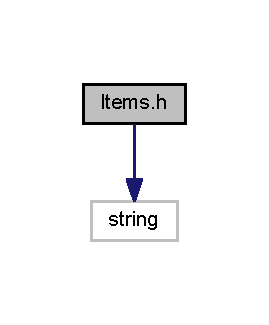
\includegraphics[width=129pt]{_items_8h__incl}
\end{center}
\end{figure}
Граф файлов, в которые включается этот файл\+:
\nopagebreak
\begin{figure}[H]
\begin{center}
\leavevmode
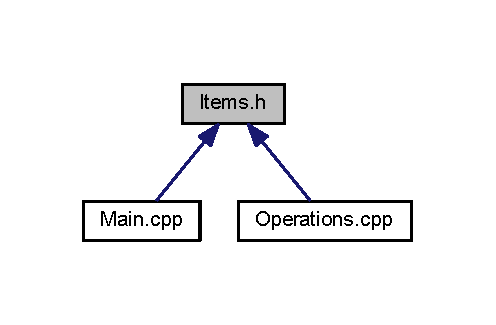
\includegraphics[width=238pt]{_items_8h__dep__incl}
\end{center}
\end{figure}
\subsection*{Функции}
\begin{DoxyCompactItemize}
\item 
std\+::string \hyperlink{_items_8h_ac7f6531a9ecd51bc1ac40c3d6a142c87}{s\+\_\+mainmenu} ()
\item 
std\+::string \hyperlink{_items_8h_aff329d8d7665b0b0778374dc958f84e1}{s\+\_\+querymenu} (std\+::string item)
\item 
std\+::string \hyperlink{_items_8h_abd9bea227cb7ce61cb32dc1c9e4d2104}{s\+\_\+checkagreement} ()
\item 
void \hyperlink{_items_8h_ae0f9a7fdce9e3a275336f70656c0c4fc}{v\+\_\+manual} ()
\end{DoxyCompactItemize}


\subsection{Подробное описание}
Заголовочный файл с подключением меню. 

\begin{DoxyAuthor}{Автор}
Sava\+Lione 
\end{DoxyAuthor}


\subsection{Функции}
\mbox{\Hypertarget{_items_8h_abd9bea227cb7ce61cb32dc1c9e4d2104}\label{_items_8h_abd9bea227cb7ce61cb32dc1c9e4d2104}} 
\index{Items.\+h@{Items.\+h}!s\+\_\+checkagreement@{s\+\_\+checkagreement}}
\index{s\+\_\+checkagreement@{s\+\_\+checkagreement}!Items.\+h@{Items.\+h}}
\subsubsection{\texorpdfstring{s\+\_\+checkagreement()}{s\_checkagreement()}}
{\footnotesize\ttfamily std\+::string s\+\_\+checkagreement (\begin{DoxyParamCaption}{ }\end{DoxyParamCaption})}

Проверка согласия пользователя с пользовательским соглашением. \begin{DoxyReturn}{Возвращает}
Выбранный пункт меню. 
\end{DoxyReturn}


См. определение в файле Items.\+cpp строка 87

\mbox{\Hypertarget{_items_8h_ac7f6531a9ecd51bc1ac40c3d6a142c87}\label{_items_8h_ac7f6531a9ecd51bc1ac40c3d6a142c87}} 
\index{Items.\+h@{Items.\+h}!s\+\_\+mainmenu@{s\+\_\+mainmenu}}
\index{s\+\_\+mainmenu@{s\+\_\+mainmenu}!Items.\+h@{Items.\+h}}
\subsubsection{\texorpdfstring{s\+\_\+mainmenu()}{s\_mainmenu()}}
{\footnotesize\ttfamily std\+::string s\+\_\+mainmenu (\begin{DoxyParamCaption}{ }\end{DoxyParamCaption})}

Главное меню. \begin{DoxyReturn}{Возвращает}
Выбранный пункт меню. 
\end{DoxyReturn}


См. определение в файле Items.\+cpp строка 27

\mbox{\Hypertarget{_items_8h_aff329d8d7665b0b0778374dc958f84e1}\label{_items_8h_aff329d8d7665b0b0778374dc958f84e1}} 
\index{Items.\+h@{Items.\+h}!s\+\_\+querymenu@{s\+\_\+querymenu}}
\index{s\+\_\+querymenu@{s\+\_\+querymenu}!Items.\+h@{Items.\+h}}
\subsubsection{\texorpdfstring{s\+\_\+querymenu()}{s\_querymenu()}}
{\footnotesize\ttfamily std\+::string s\+\_\+querymenu (\begin{DoxyParamCaption}\item[{std\+::string}]{item }\end{DoxyParamCaption})}

Сообщение с вопросом для пользователя. 
\begin{DoxyParams}[1]{Аргументы}
\mbox{\tt in}  & {\em item} & Строка до выполнения модуля меню. \\
\hline
\end{DoxyParams}
\begin{DoxyReturn}{Возвращает}
Выбранный пункт меню. 
\end{DoxyReturn}
\mbox{\Hypertarget{_items_8h_ae0f9a7fdce9e3a275336f70656c0c4fc}\label{_items_8h_ae0f9a7fdce9e3a275336f70656c0c4fc}} 
\index{Items.\+h@{Items.\+h}!v\+\_\+manual@{v\+\_\+manual}}
\index{v\+\_\+manual@{v\+\_\+manual}!Items.\+h@{Items.\+h}}
\subsubsection{\texorpdfstring{v\+\_\+manual()}{v\_manual()}}
{\footnotesize\ttfamily void v\+\_\+manual (\begin{DoxyParamCaption}{ }\end{DoxyParamCaption})}

Инструкция к программе. 

См. определение в файле Items.\+cpp строка 113


\hypertarget{_logger_8cpp}{}\section{Файл Logger.\+cpp}
\label{_logger_8cpp}\index{Logger.\+cpp@{Logger.\+cpp}}


Модуль логирования  


{\ttfamily \#include $<$string$>$}\newline
{\ttfamily \#include $<$fstream$>$}\newline
{\ttfamily \#include $<$thread$>$}\newline
{\ttfamily \#include $<$windows.\+h$>$}\newline
{\ttfamily \#include $<$stdio.\+h$>$}\newline
{\ttfamily \#include \char`\"{}Logger.\+h\char`\"{}}\newline
{\ttfamily \#include \char`\"{}Settings.\+h\char`\"{}}\newline
Граф включаемых заголовочных файлов для Logger.\+cpp\+:\nopagebreak
\begin{figure}[H]
\begin{center}
\leavevmode
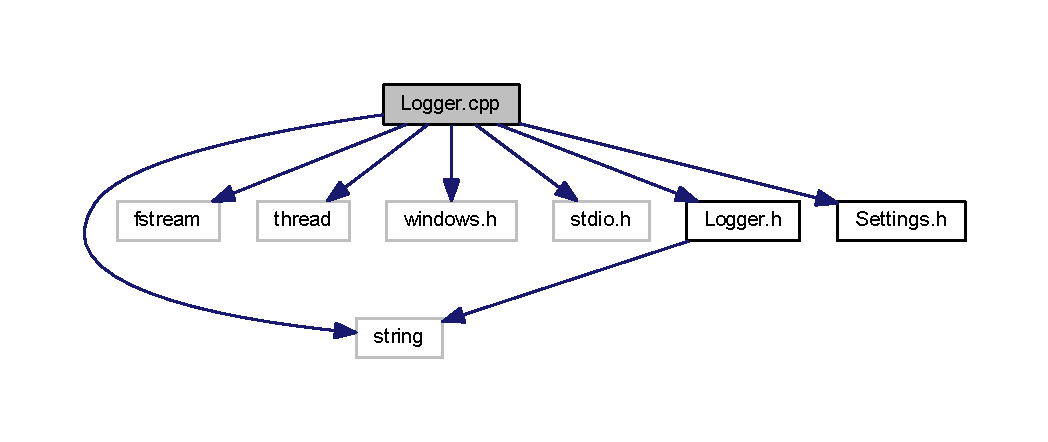
\includegraphics[width=350pt]{_logger_8cpp__incl}
\end{center}
\end{figure}
\subsection*{Функции}
\begin{DoxyCompactItemize}
\item 
void \hyperlink{_logger_8cpp_a37ded7634d8547536bbd135208109766}{log\+\_\+thr} (string \&s, string \&level)
\item 
void \hyperlink{_logger_8cpp_a85cbef1702d055318336f0f3a5036959}{log} (string level, string s)
\end{DoxyCompactItemize}


\subsection{Подробное описание}
Модуль логирования 


\begin{DoxyCode}
Логгер
Логгирование сообщений в файл logger.log
Уровеней лога - 3
Уровень 0:
Вывод сообщений вида:
    [                   ] \{MESSAGE\}
Применение:
    Обработка простых сообщений, без времени и префикса ([PREFIX])
Уровень 1:
Вывод сообщений вида:
    [\{YEAR\}/\{MONTH\}/\{DAY\} \{HOUR\}:\{MINUTE\}:\{SECOND\}] [LOG] \{MESSAGE\}
Применение:
    Обработка простых сообщений(загрузка модуля, отключение модуля, вход в программу, выход из программы и 
      тд.) С временем и префиксом ([LOG])
Уровень 2:
Вывод сообщений вида:
    [\{YEAR\}/\{MONTH\}/\{DAY\} \{HOUR\}:\{MINUTE\}:\{SECOND\}] [WARN] \{MESSAGE\}
Применение:
    Обработка важных сообщений ошибки(не удачная загрузка модуля, не удачный вход в программу, экстренный 
      выход из программы и тд.) С временем и префиксом ([WARN])
\end{DoxyCode}
 

\subsection{Функции}
\mbox{\Hypertarget{_logger_8cpp_a85cbef1702d055318336f0f3a5036959}\label{_logger_8cpp_a85cbef1702d055318336f0f3a5036959}} 
\index{Logger.\+cpp@{Logger.\+cpp}!log@{log}}
\index{log@{log}!Logger.\+cpp@{Logger.\+cpp}}
\subsubsection{\texorpdfstring{log()}{log()}}
{\footnotesize\ttfamily void log (\begin{DoxyParamCaption}\item[{string}]{level,  }\item[{string}]{s }\end{DoxyParamCaption})}

Логгирование сообщений в файл logger.\+log 
\begin{DoxyParams}[1]{Аргументы}
\mbox{\tt in}  & {\em level} & Уровень логирования \\
\hline
\mbox{\tt in}  & {\em s} & Логируемая информация \\
\hline
\end{DoxyParams}
\begin{Desc}
\item[Примеры\+: ]\par
\hyperlink{log_8cpp-example}{log.\+cpp}.\end{Desc}
\mbox{\Hypertarget{_logger_8cpp_a37ded7634d8547536bbd135208109766}\label{_logger_8cpp_a37ded7634d8547536bbd135208109766}} 
\index{Logger.\+cpp@{Logger.\+cpp}!log\+\_\+thr@{log\+\_\+thr}}
\index{log\+\_\+thr@{log\+\_\+thr}!Logger.\+cpp@{Logger.\+cpp}}
\subsubsection{\texorpdfstring{log\+\_\+thr()}{log\_thr()}}
{\footnotesize\ttfamily void log\+\_\+thr (\begin{DoxyParamCaption}\item[{string \&}]{s,  }\item[{string \&}]{level }\end{DoxyParamCaption})}

Функция, для записи лога в файл 
\begin{DoxyParams}[1]{Аргументы}
\mbox{\tt in}  & {\em \&s} & Передача ссылки с сообщением для логирования \\
\hline
\mbox{\tt in}  & {\em \&level} & Передача ссылки с уровнем логирования \\
\hline
\end{DoxyParams}

\hypertarget{_logger_8h}{}\section{Файл Logger.\+h}
\label{_logger_8h}\index{Logger.\+h@{Logger.\+h}}


Заголовочный файл с подключением модуля логирования.  


{\ttfamily \#include $<$string$>$}\newline
Граф включаемых заголовочных файлов для Logger.\+h\+:
\nopagebreak
\begin{figure}[H]
\begin{center}
\leavevmode
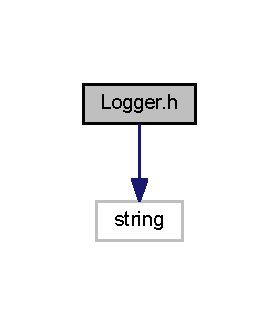
\includegraphics[width=134pt]{_logger_8h__incl}
\end{center}
\end{figure}
Граф файлов, в которые включается этот файл\+:
\nopagebreak
\begin{figure}[H]
\begin{center}
\leavevmode
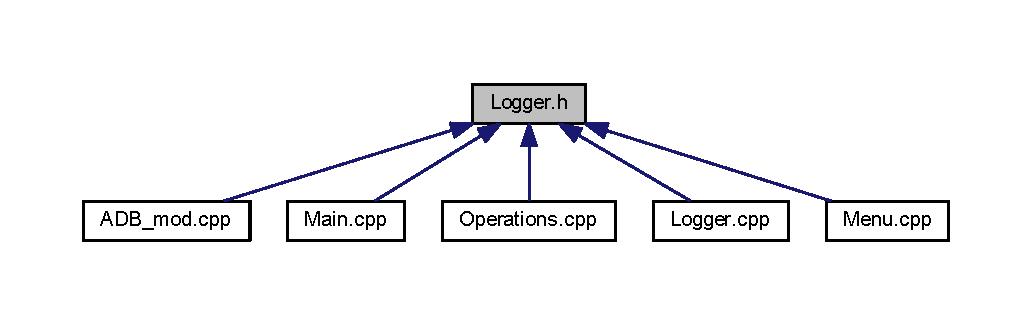
\includegraphics[width=350pt]{_logger_8h__dep__incl}
\end{center}
\end{figure}
\subsection*{Функции}
\begin{DoxyCompactItemize}
\item 
void \hyperlink{_logger_8h_ad35770e66782b0d5c63307682c5de765}{log} (std\+::string level, std\+::string s)
\end{DoxyCompactItemize}


\subsection{Подробное описание}
Заголовочный файл с подключением модуля логирования. 

\begin{DoxyAuthor}{Автор}
Sava\+Lione 
\end{DoxyAuthor}


\subsection{Функции}
\mbox{\Hypertarget{_logger_8h_ad35770e66782b0d5c63307682c5de765}\label{_logger_8h_ad35770e66782b0d5c63307682c5de765}} 
\index{Logger.\+h@{Logger.\+h}!log@{log}}
\index{log@{log}!Logger.\+h@{Logger.\+h}}
\subsubsection{\texorpdfstring{log()}{log()}}
{\footnotesize\ttfamily void log (\begin{DoxyParamCaption}\item[{std\+::string}]{level,  }\item[{std\+::string}]{s }\end{DoxyParamCaption})}

Логирование сообщений в файл logger.\+log 
\begin{DoxyParams}[1]{Аргументы}
\mbox{\tt in}  & {\em level} & Уровень логирования. \\
\hline
\mbox{\tt in}  & {\em s} & Логируемая информация. \\
\hline
\end{DoxyParams}

\hypertarget{_main_8cpp}{}\section{Файл Main.\+cpp}
\label{_main_8cpp}\index{Main.\+cpp@{Main.\+cpp}}


Главный файл программы  


{\ttfamily \#include $<$string$>$}\newline
{\ttfamily \#include \char`\"{}..\textbackslash{}core\textbackslash{}\+Operations.\+h\char`\"{}}\newline
{\ttfamily \#include \char`\"{}..\textbackslash{}io\textbackslash{}\+Logger.\+h\char`\"{}}\newline
{\ttfamily \#include \char`\"{}..\textbackslash{}ui\textbackslash{}\+Menu.\+h\char`\"{}}\newline
{\ttfamily \#include \char`\"{}..\textbackslash{}ui\textbackslash{}\+Items.\+h\char`\"{}}\newline
Граф включаемых заголовочных файлов для Main.\+cpp\+:
\nopagebreak
\begin{figure}[H]
\begin{center}
\leavevmode
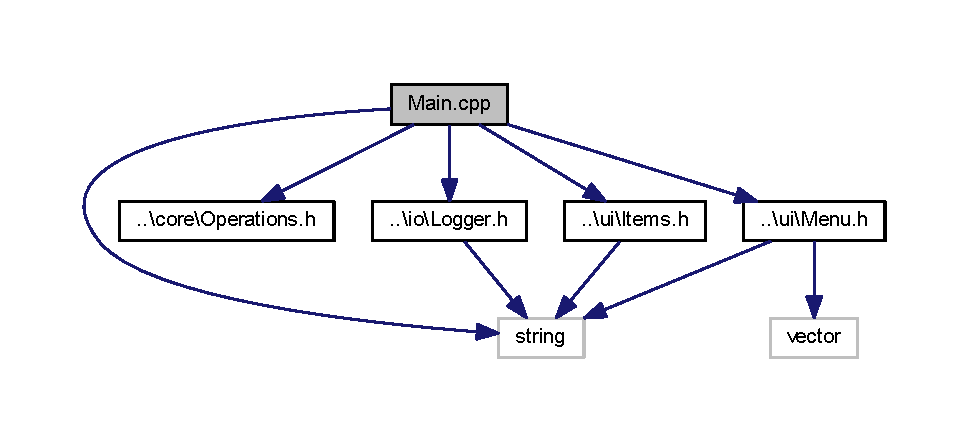
\includegraphics[width=350pt]{_main_8cpp__incl}
\end{center}
\end{figure}
\subsection*{Функции}
\begin{DoxyCompactItemize}
\item 
int \hyperlink{_main_8cpp_ae66f6b31b5ad750f1fe042a706a4e3d4}{main} ()
\end{DoxyCompactItemize}


\subsection{Подробное описание}
Главный файл программы 

\begin{DoxyAuthor}{Автор}
Sava\+Lione 
\end{DoxyAuthor}


\subsection{Функции}
\mbox{\Hypertarget{_main_8cpp_ae66f6b31b5ad750f1fe042a706a4e3d4}\label{_main_8cpp_ae66f6b31b5ad750f1fe042a706a4e3d4}} 
\index{Main.\+cpp@{Main.\+cpp}!main@{main}}
\index{main@{main}!Main.\+cpp@{Main.\+cpp}}
\subsubsection{\texorpdfstring{main()}{main()}}
{\footnotesize\ttfamily int main (\begin{DoxyParamCaption}{ }\end{DoxyParamCaption})}

\begin{DoxyReturn}{Возвращает}
Код завершения программы Вызов программы компилятором 
\end{DoxyReturn}
\begin{Desc}
\item[Примеры\+: ]\par
\hyperlink{color_8cpp-example}{color.\+cpp}, \hyperlink{constants_8cpp-example}{constants.\+cpp}, \hyperlink{items_8cpp-example}{items.\+cpp}, \hyperlink{log_8cpp-example}{log.\+cpp}, \hyperlink{menu_8cpp-example}{menu.\+cpp}, \hyperlink{_operations_8cpp-example}{Operations.\+cpp}, \hyperlink{_operations__initialization_8cpp-example}{Operations\+\_\+\+Initialization.\+cpp}, \hyperlink{settings_8cpp-example}{settings.\+cpp} и \hyperlink{templates_8cpp-example}{templates.\+cpp}.\end{Desc}


См. определение в файле Main.\+cpp строка 19


\hypertarget{_menu_8cpp}{}\section{Файл Menu.\+cpp}
\label{_menu_8cpp}\index{Menu.\+cpp@{Menu.\+cpp}}


Модуль создания меню.  


{\ttfamily \#include $<$iostream$>$}\newline
{\ttfamily \#include $<$conio.\+h$>$}\newline
{\ttfamily \#include $<$string$>$}\newline
{\ttfamily \#include $<$Windows.\+h$>$}\newline
{\ttfamily \#include \char`\"{}..\textbackslash{}core\textbackslash{}\+Constants.\+h\char`\"{}}\newline
{\ttfamily \#include \char`\"{}..\textbackslash{}core\textbackslash{}\+Color.\+h\char`\"{}}\newline
{\ttfamily \#include \char`\"{}..\textbackslash{}ui\textbackslash{}\+Menu.\+h\char`\"{}}\newline
{\ttfamily \#include \char`\"{}..\textbackslash{}io\textbackslash{}\+Logger.\+h\char`\"{}}\newline
Граф включаемых заголовочных файлов для Menu.\+cpp\+:
\nopagebreak
\begin{figure}[H]
\begin{center}
\leavevmode
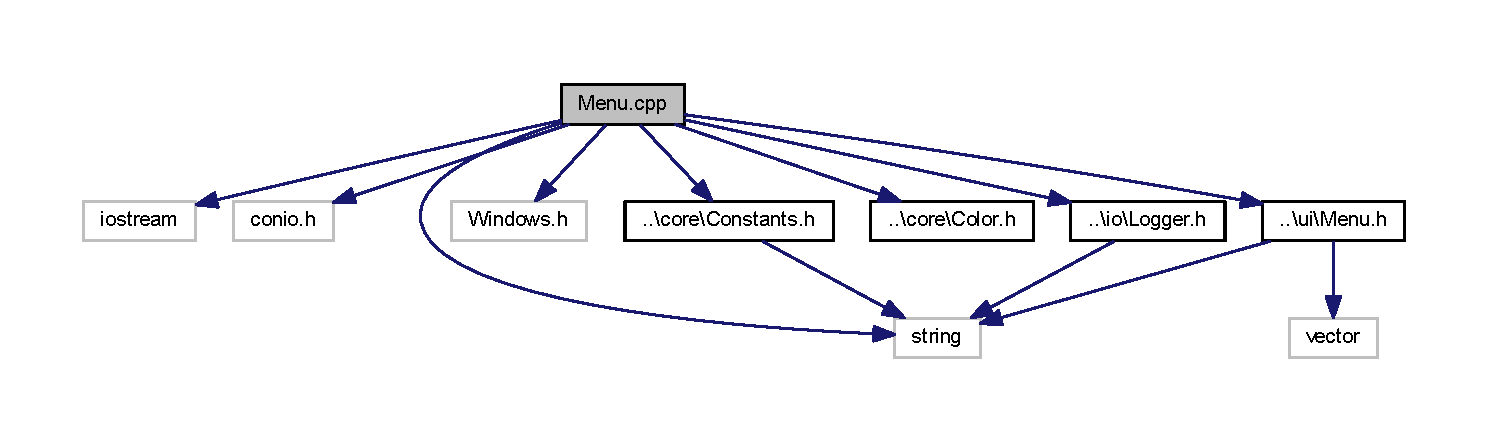
\includegraphics[width=350pt]{_menu_8cpp__incl}
\end{center}
\end{figure}
\subsection*{Функции}
\begin{DoxyCompactItemize}
\item 
string \hyperlink{_menu_8cpp_aafe15d5b7f6c3bf3fe4563fdf6810633}{s\+\_\+menu\+\_\+choice} (size\+\_\+t choice, \hyperlink{structmenu__s}{menu\+\_\+s} menu)
\item 
string \hyperlink{_menu_8cpp_a20a38c5c97dbebd634a7b5c71fcd6120}{s\+\_\+menu} (\hyperlink{structmenu__s}{menu\+\_\+s} menu)
\item 
void \hyperlink{_menu_8cpp_a7167f5c196fc5e167bfabde1a730e81d}{pause} ()
\item 
void \hyperlink{_menu_8cpp_a540f8b6f2205a3bcf98d2b8f81e8aa09}{v\+\_\+exit} ()
\item 
void \hyperlink{_menu_8cpp_ab957e5514a924cccac4e53b2a576d063}{v\+\_\+loadscale} (size\+\_\+t position)
\end{DoxyCompactItemize}


\subsection{Подробное описание}
Модуль создания меню. 



\subsection{Функции}
\mbox{\Hypertarget{_menu_8cpp_a7167f5c196fc5e167bfabde1a730e81d}\label{_menu_8cpp_a7167f5c196fc5e167bfabde1a730e81d}} 
\index{Menu.\+cpp@{Menu.\+cpp}!pause@{pause}}
\index{pause@{pause}!Menu.\+cpp@{Menu.\+cpp}}
\subsubsection{\texorpdfstring{pause()}{pause()}}
{\footnotesize\ttfamily void pause (\begin{DoxyParamCaption}{ }\end{DoxyParamCaption})}

Паузка до нажатия любой клавиши. 

См. определение в файле Menu.\+cpp строка 107

\mbox{\Hypertarget{_menu_8cpp_a20a38c5c97dbebd634a7b5c71fcd6120}\label{_menu_8cpp_a20a38c5c97dbebd634a7b5c71fcd6120}} 
\index{Menu.\+cpp@{Menu.\+cpp}!s\+\_\+menu@{s\+\_\+menu}}
\index{s\+\_\+menu@{s\+\_\+menu}!Menu.\+cpp@{Menu.\+cpp}}
\subsubsection{\texorpdfstring{s\+\_\+menu()}{s\_menu()}}
{\footnotesize\ttfamily string s\+\_\+menu (\begin{DoxyParamCaption}\item[{\hyperlink{structmenu__s}{menu\+\_\+s}}]{menu }\end{DoxyParamCaption})}

Модуль создания меню. 
\begin{DoxyParams}[1]{Аргументы}
\mbox{\tt in}  & {\em menu} & Список с параметрами создаваемого меню. \\
\hline
\end{DoxyParams}
\begin{DoxyReturn}{Возвращает}
Выбранный пункт меню. 
\end{DoxyReturn}
\begin{Desc}
\item[Примеры\+: ]\par
\hyperlink{menu_8cpp-example}{menu.\+cpp}.\end{Desc}


См. определение в файле Menu.\+cpp строка 61

\mbox{\Hypertarget{_menu_8cpp_aafe15d5b7f6c3bf3fe4563fdf6810633}\label{_menu_8cpp_aafe15d5b7f6c3bf3fe4563fdf6810633}} 
\index{Menu.\+cpp@{Menu.\+cpp}!s\+\_\+menu\+\_\+choice@{s\+\_\+menu\+\_\+choice}}
\index{s\+\_\+menu\+\_\+choice@{s\+\_\+menu\+\_\+choice}!Menu.\+cpp@{Menu.\+cpp}}
\subsubsection{\texorpdfstring{s\+\_\+menu\+\_\+choice()}{s\_menu\_choice()}}
{\footnotesize\ttfamily string s\+\_\+menu\+\_\+choice (\begin{DoxyParamCaption}\item[{size\+\_\+t}]{choice,  }\item[{\hyperlink{structmenu__s}{menu\+\_\+s}}]{menu }\end{DoxyParamCaption})}

Отрисовка модуля создания меню. 
\begin{DoxyParams}[1]{Аргументы}
\mbox{\tt in}  & {\em choice} & Выбранный пункт меню. \\
\hline
\mbox{\tt in}  & {\em menu} & Список с параметрами создаваемого меню. \\
\hline
\end{DoxyParams}
\begin{DoxyReturn}{Возвращает}
Выбранный пункт меню. 
\end{DoxyReturn}


См. определение в файле Menu.\+cpp строка 31

\mbox{\Hypertarget{_menu_8cpp_a540f8b6f2205a3bcf98d2b8f81e8aa09}\label{_menu_8cpp_a540f8b6f2205a3bcf98d2b8f81e8aa09}} 
\index{Menu.\+cpp@{Menu.\+cpp}!v\+\_\+exit@{v\+\_\+exit}}
\index{v\+\_\+exit@{v\+\_\+exit}!Menu.\+cpp@{Menu.\+cpp}}
\subsubsection{\texorpdfstring{v\+\_\+exit()}{v\_exit()}}
{\footnotesize\ttfamily void v\+\_\+exit (\begin{DoxyParamCaption}{ }\end{DoxyParamCaption})}

Выход из программы. Вывод текста. 

См. определение в файле Menu.\+cpp строка 114

\mbox{\Hypertarget{_menu_8cpp_ab957e5514a924cccac4e53b2a576d063}\label{_menu_8cpp_ab957e5514a924cccac4e53b2a576d063}} 
\index{Menu.\+cpp@{Menu.\+cpp}!v\+\_\+loadscale@{v\+\_\+loadscale}}
\index{v\+\_\+loadscale@{v\+\_\+loadscale}!Menu.\+cpp@{Menu.\+cpp}}
\subsubsection{\texorpdfstring{v\+\_\+loadscale()}{v\_loadscale()}}
{\footnotesize\ttfamily void v\+\_\+loadscale (\begin{DoxyParamCaption}\item[{size\+\_\+t}]{position }\end{DoxyParamCaption})}

Шкала загрузки 
\begin{DoxyParams}[1]{Аргументы}
\mbox{\tt in}  & {\em position} & значение до которого отрисовывать шкалу. \\
\hline
\end{DoxyParams}


См. определение в файле Menu.\+cpp строка 128


\hypertarget{_menu_8h}{}\section{Файл Menu.\+h}
\label{_menu_8h}\index{Menu.\+h@{Menu.\+h}}


Заголовочный файл с подключением модуля создания меню.  


{\ttfamily \#include $<$string$>$}\newline
{\ttfamily \#include $<$vector$>$}\newline
Граф включаемых заголовочных файлов для Menu.\+h\+:
\nopagebreak
\begin{figure}[H]
\begin{center}
\leavevmode
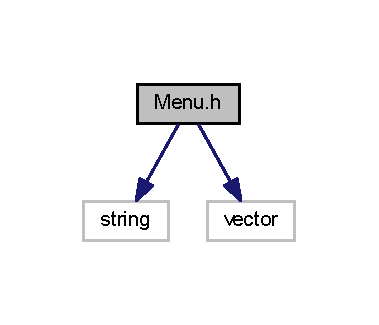
\includegraphics[width=182pt]{_menu_8h__incl}
\end{center}
\end{figure}
Граф файлов, в которые включается этот файл\+:
\nopagebreak
\begin{figure}[H]
\begin{center}
\leavevmode
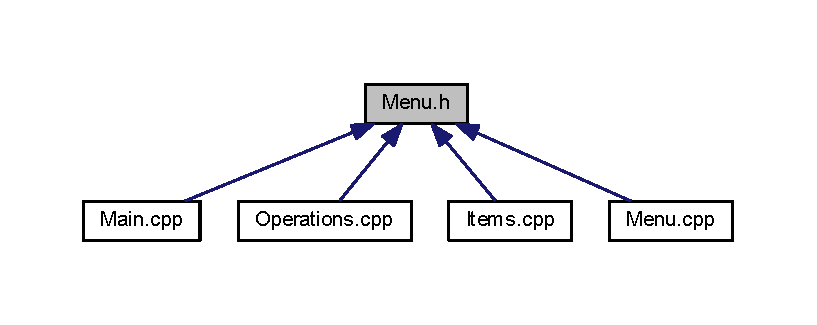
\includegraphics[width=350pt]{_menu_8h__dep__incl}
\end{center}
\end{figure}
\subsection*{Классы}
\begin{DoxyCompactItemize}
\item 
struct \hyperlink{structmenu__s}{menu\+\_\+s}
\end{DoxyCompactItemize}
\subsection*{Функции}
\begin{DoxyCompactItemize}
\item 
std\+::string \hyperlink{_menu_8h_a7e6e7063d214256725a790c495d5c9da}{s\+\_\+menu} (\hyperlink{structmenu__s}{menu\+\_\+s} menu)
\item 
void \hyperlink{_menu_8h_a7167f5c196fc5e167bfabde1a730e81d}{pause} ()
\item 
void \hyperlink{_menu_8h_a540f8b6f2205a3bcf98d2b8f81e8aa09}{v\+\_\+exit} ()
\item 
void \hyperlink{_menu_8h_ab957e5514a924cccac4e53b2a576d063}{v\+\_\+loadscale} (size\+\_\+t position)
\end{DoxyCompactItemize}


\subsection{Подробное описание}
Заголовочный файл с подключением модуля создания меню. 

\begin{DoxyAuthor}{Автор}
Sava\+Lione 
\end{DoxyAuthor}


\subsection{Функции}
\mbox{\Hypertarget{_menu_8h_a7167f5c196fc5e167bfabde1a730e81d}\label{_menu_8h_a7167f5c196fc5e167bfabde1a730e81d}} 
\index{Menu.\+h@{Menu.\+h}!pause@{pause}}
\index{pause@{pause}!Menu.\+h@{Menu.\+h}}
\subsubsection{\texorpdfstring{pause()}{pause()}}
{\footnotesize\ttfamily void pause (\begin{DoxyParamCaption}{ }\end{DoxyParamCaption})}

Паузка до нажатия любой клавиши. 

См. определение в файле Menu.\+cpp строка 107

\mbox{\Hypertarget{_menu_8h_a7e6e7063d214256725a790c495d5c9da}\label{_menu_8h_a7e6e7063d214256725a790c495d5c9da}} 
\index{Menu.\+h@{Menu.\+h}!s\+\_\+menu@{s\+\_\+menu}}
\index{s\+\_\+menu@{s\+\_\+menu}!Menu.\+h@{Menu.\+h}}
\subsubsection{\texorpdfstring{s\+\_\+menu()}{s\_menu()}}
{\footnotesize\ttfamily std\+::string s\+\_\+menu (\begin{DoxyParamCaption}\item[{\hyperlink{structmenu__s}{menu\+\_\+s}}]{menu }\end{DoxyParamCaption})}

Модуль создания меню. 
\begin{DoxyParams}[1]{Аргументы}
\mbox{\tt in}  & {\em menu} & Список с параметрами создаваемого меню. \\
\hline
\end{DoxyParams}
\begin{DoxyReturn}{Возвращает}
Выбранный пункт меню. 
\end{DoxyReturn}


См. определение в файле Menu.\+cpp строка 61

\mbox{\Hypertarget{_menu_8h_a540f8b6f2205a3bcf98d2b8f81e8aa09}\label{_menu_8h_a540f8b6f2205a3bcf98d2b8f81e8aa09}} 
\index{Menu.\+h@{Menu.\+h}!v\+\_\+exit@{v\+\_\+exit}}
\index{v\+\_\+exit@{v\+\_\+exit}!Menu.\+h@{Menu.\+h}}
\subsubsection{\texorpdfstring{v\+\_\+exit()}{v\_exit()}}
{\footnotesize\ttfamily void v\+\_\+exit (\begin{DoxyParamCaption}{ }\end{DoxyParamCaption})}

Выход из программы. Вывод текста. 

См. определение в файле Menu.\+cpp строка 114

\mbox{\Hypertarget{_menu_8h_ab957e5514a924cccac4e53b2a576d063}\label{_menu_8h_ab957e5514a924cccac4e53b2a576d063}} 
\index{Menu.\+h@{Menu.\+h}!v\+\_\+loadscale@{v\+\_\+loadscale}}
\index{v\+\_\+loadscale@{v\+\_\+loadscale}!Menu.\+h@{Menu.\+h}}
\subsubsection{\texorpdfstring{v\+\_\+loadscale()}{v\_loadscale()}}
{\footnotesize\ttfamily void v\+\_\+loadscale (\begin{DoxyParamCaption}\item[{size\+\_\+t}]{position }\end{DoxyParamCaption})}

Шкала загрузки. 
\begin{DoxyParams}[1]{Аргументы}
\mbox{\tt in}  & {\em position} & значение до которого отрисовывать шкалу.\\
\hline
\end{DoxyParams}
Шкала загрузки 
\begin{DoxyParams}[1]{Аргументы}
\mbox{\tt in}  & {\em position} & значение до которого отрисовывать шкалу. \\
\hline
\end{DoxyParams}


См. определение в файле Menu.\+cpp строка 128


\hypertarget{_operations_8cpp}{}\section{Файл Operations.\+cpp}
\label{_operations_8cpp}\index{Operations.\+cpp@{Operations.\+cpp}}


Модуль проверки стандартных файлов программы и вызова алгоритма рутирования.  


{\ttfamily \#include $<$string$>$}\newline
{\ttfamily \#include $<$io.\+h$>$}\newline
{\ttfamily \#include $<$Windows.\+h$>$}\newline
{\ttfamily \#include \char`\"{}..\textbackslash{}core\textbackslash{}\+A\+D\+B\+\_\+mod.\+h\char`\"{}}\newline
{\ttfamily \#include \char`\"{}..\textbackslash{}core\textbackslash{}\+Constants.\+h\char`\"{}}\newline
{\ttfamily \#include \char`\"{}..\textbackslash{}core\textbackslash{}\+Operations.\+h\char`\"{}}\newline
{\ttfamily \#include \char`\"{}..\textbackslash{}io\textbackslash{}\+Logger.\+h\char`\"{}}\newline
{\ttfamily \#include \char`\"{}..\textbackslash{}io\textbackslash{}\+Templates.\+h\char`\"{}}\newline
{\ttfamily \#include \char`\"{}..\textbackslash{}ui\textbackslash{}\+Menu.\+h\char`\"{}}\newline
{\ttfamily \#include \char`\"{}..\textbackslash{}ui\textbackslash{}\+Items.\+h\char`\"{}}\newline
Граф включаемых заголовочных файлов для Operations.\+cpp\+:
\nopagebreak
\begin{figure}[H]
\begin{center}
\leavevmode
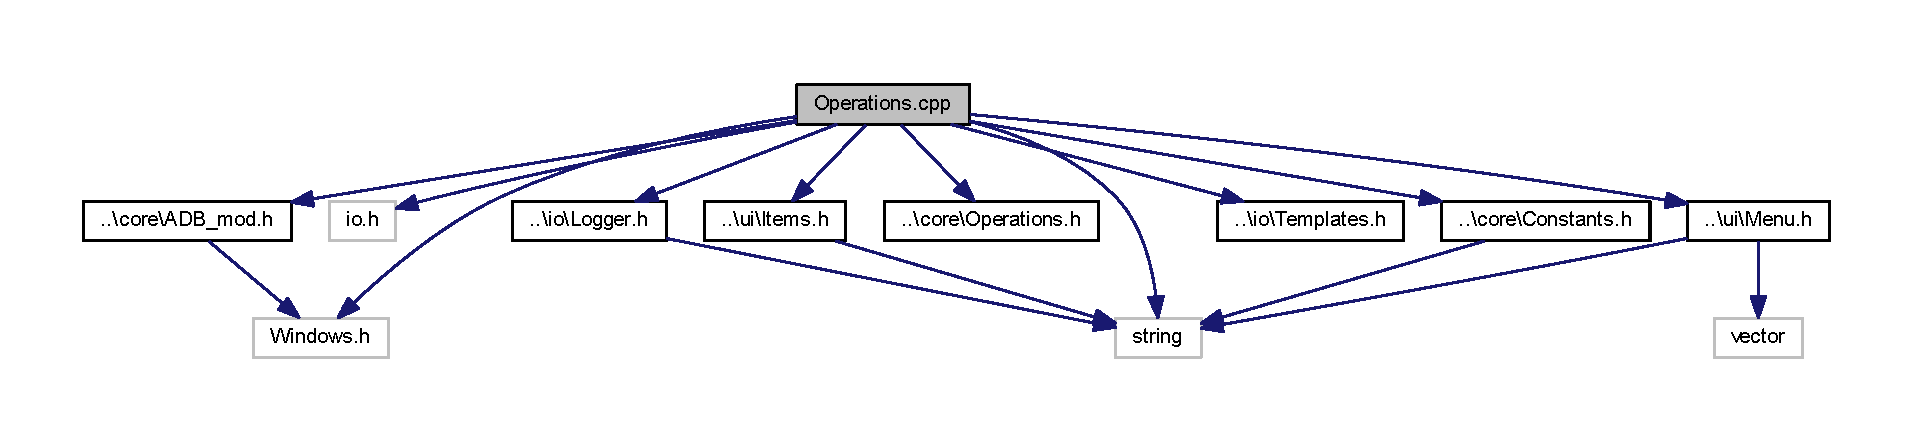
\includegraphics[width=350pt]{_operations_8cpp__incl}
\end{center}
\end{figure}
\subsection*{Функции}
\begin{DoxyCompactItemize}
\item 
void \hyperlink{_operations_8cpp_a61271965777637ec3d70f6d7ab0a466a}{v\+\_\+initialization\+\_\+logger\+\_\+log} ()
\begin{DoxyCompactList}\small\item\em Проверка файла logger.\+log. \end{DoxyCompactList}\item 
void \hyperlink{_operations_8cpp_a9f137f3ae0426a1e7c1a398ad930dc70}{v\+\_\+initialization\+\_\+settings\+\_\+ini} ()
\begin{DoxyCompactList}\small\item\em Проверка файла settings.\+ini. \end{DoxyCompactList}\item 
void \hyperlink{_operations_8cpp_a784c09041cf40075e8eb016a2d8419d6}{root} ()
\item 
bool \hyperlink{_operations_8cpp_a06ba6d957eba855cc9f88ce7ac641722}{b\+\_\+file\+\_\+exists} (const char $\ast$ch\+\_\+file\+\_\+name)
\item 
int \hyperlink{_operations_8cpp_a5f44f09549aae42fa22e71e761b40abc}{i\+\_\+checking\+\_\+files} ()
\item 
void \hyperlink{_operations_8cpp_a11b373fd61e18cd28810a5b607e1749a}{v\+\_\+initialization} ()
\end{DoxyCompactItemize}


\subsection{Подробное описание}
Модуль проверки стандартных файлов программы и вызова алгоритма рутирования. 

Модуль проверяет наличие стандартных файлов программы и рутирует аппарат.

Файлы\+: \begin{DoxyVerb}logger.log - вывод логера.

rules.txt - правила программы, с которыми должен согласиться пользователь.

settings.ini - файл настроек.\end{DoxyVerb}


\subsection{Функции}
\mbox{\Hypertarget{_operations_8cpp_a06ba6d957eba855cc9f88ce7ac641722}\label{_operations_8cpp_a06ba6d957eba855cc9f88ce7ac641722}} 
\index{Operations.\+cpp@{Operations.\+cpp}!b\+\_\+file\+\_\+exists@{b\+\_\+file\+\_\+exists}}
\index{b\+\_\+file\+\_\+exists@{b\+\_\+file\+\_\+exists}!Operations.\+cpp@{Operations.\+cpp}}
\subsubsection{\texorpdfstring{b\+\_\+file\+\_\+exists()}{b\_file\_exists()}}
{\footnotesize\ttfamily bool b\+\_\+file\+\_\+exists (\begin{DoxyParamCaption}\item[{const char $\ast$}]{ch\+\_\+file\+\_\+name }\end{DoxyParamCaption})}

Вызов модуля проверки файла на наличие в папке. 
\begin{DoxyParams}[1]{Аргументы}
\mbox{\tt in}  & {\em ch\+\_\+file\+\_\+name} & Путь и файл, для проверки. \\
\hline
\end{DoxyParams}
\begin{DoxyReturn}{Возвращает}
наличие файла. 
\end{DoxyReturn}
\begin{Desc}
\item[Примеры\+: ]\par
\hyperlink{_operations__initialization_8cpp-example}{Operations\+\_\+\+Initialization.\+cpp}.\end{Desc}


См. определение в файле Operations.\+cpp строка 54

\mbox{\Hypertarget{_operations_8cpp_a5f44f09549aae42fa22e71e761b40abc}\label{_operations_8cpp_a5f44f09549aae42fa22e71e761b40abc}} 
\index{Operations.\+cpp@{Operations.\+cpp}!i\+\_\+checking\+\_\+files@{i\+\_\+checking\+\_\+files}}
\index{i\+\_\+checking\+\_\+files@{i\+\_\+checking\+\_\+files}!Operations.\+cpp@{Operations.\+cpp}}
\subsubsection{\texorpdfstring{i\+\_\+checking\+\_\+files()}{i\_checking\_files()}}
{\footnotesize\ttfamily int i\+\_\+checking\+\_\+files (\begin{DoxyParamCaption}{ }\end{DoxyParamCaption})}

Вызов модуля проверки файлов. \begin{DoxyReturn}{Возвращает}
0 -\/ неуспешная проверка файлов. 1 -\/ успешная проверка файлов. 
\end{DoxyReturn}
\begin{Desc}
\item[Примеры\+: ]\par
\hyperlink{_operations_8cpp-example}{Operations.\+cpp} и \hyperlink{_operations__initialization_8cpp-example}{Operations\+\_\+\+Initialization.\+cpp}.\end{Desc}


См. определение в файле Operations.\+cpp строка 65

\mbox{\Hypertarget{_operations_8cpp_a784c09041cf40075e8eb016a2d8419d6}\label{_operations_8cpp_a784c09041cf40075e8eb016a2d8419d6}} 
\index{Operations.\+cpp@{Operations.\+cpp}!root@{root}}
\index{root@{root}!Operations.\+cpp@{Operations.\+cpp}}
\subsubsection{\texorpdfstring{root()}{root()}}
{\footnotesize\ttfamily void root (\begin{DoxyParamCaption}{ }\end{DoxyParamCaption})}

Вызов алгоритма рутирования. \begin{Desc}
\item[Примеры\+: ]\par
\hyperlink{_operations_8cpp-example}{Operations.\+cpp}.\end{Desc}


См. определение в файле Operations.\+cpp строка 40

\mbox{\Hypertarget{_operations_8cpp_a11b373fd61e18cd28810a5b607e1749a}\label{_operations_8cpp_a11b373fd61e18cd28810a5b607e1749a}} 
\index{Operations.\+cpp@{Operations.\+cpp}!v\+\_\+initialization@{v\+\_\+initialization}}
\index{v\+\_\+initialization@{v\+\_\+initialization}!Operations.\+cpp@{Operations.\+cpp}}
\subsubsection{\texorpdfstring{v\+\_\+initialization()}{v\_initialization()}}
{\footnotesize\ttfamily void v\+\_\+initialization (\begin{DoxyParamCaption}{ }\end{DoxyParamCaption})}

Функция проверяет наличие 3 стандартных файлов программы \begin{DoxyVerb}logger.log

rules.txt

settings.ini\end{DoxyVerb}
 \begin{Desc}
\item[Примеры\+: ]\par
\hyperlink{_operations__initialization_8cpp-example}{Operations\+\_\+\+Initialization.\+cpp}.\end{Desc}


См. определение в файле Operations.\+cpp строка 112

\mbox{\Hypertarget{_operations_8cpp_a61271965777637ec3d70f6d7ab0a466a}\label{_operations_8cpp_a61271965777637ec3d70f6d7ab0a466a}} 
\index{Operations.\+cpp@{Operations.\+cpp}!v\+\_\+initialization\+\_\+logger\+\_\+log@{v\+\_\+initialization\+\_\+logger\+\_\+log}}
\index{v\+\_\+initialization\+\_\+logger\+\_\+log@{v\+\_\+initialization\+\_\+logger\+\_\+log}!Operations.\+cpp@{Operations.\+cpp}}
\subsubsection{\texorpdfstring{v\+\_\+initialization\+\_\+logger\+\_\+log()}{v\_initialization\_logger\_log()}}
{\footnotesize\ttfamily void v\+\_\+initialization\+\_\+logger\+\_\+log (\begin{DoxyParamCaption}{ }\end{DoxyParamCaption})}



Проверка файла logger.\+log. 

Проверка файла logger.\+log

При отсутствии файла создаёт его.

При наличии файла пропуск.

Всё логируется. 

См. определение в файле Operations.\+cpp строка 132

\mbox{\Hypertarget{_operations_8cpp_a9f137f3ae0426a1e7c1a398ad930dc70}\label{_operations_8cpp_a9f137f3ae0426a1e7c1a398ad930dc70}} 
\index{Operations.\+cpp@{Operations.\+cpp}!v\+\_\+initialization\+\_\+settings\+\_\+ini@{v\+\_\+initialization\+\_\+settings\+\_\+ini}}
\index{v\+\_\+initialization\+\_\+settings\+\_\+ini@{v\+\_\+initialization\+\_\+settings\+\_\+ini}!Operations.\+cpp@{Operations.\+cpp}}
\subsubsection{\texorpdfstring{v\+\_\+initialization\+\_\+settings\+\_\+ini()}{v\_initialization\_settings\_ini()}}
{\footnotesize\ttfamily void v\+\_\+initialization\+\_\+settings\+\_\+ini (\begin{DoxyParamCaption}{ }\end{DoxyParamCaption})}



Проверка файла settings.\+ini. 

Проверка файла settings.\+ini

При отсутствии файла создаёт его.

При наличии файла пропуск.

Всё логируется. 

См. определение в файле Operations.\+cpp строка 150


\hypertarget{_operations_8h}{}\section{Файл Operations.\+h}
\label{_operations_8h}\index{Operations.\+h@{Operations.\+h}}


Заголовочный файл с вызовом модуля проверки стандартных файлов программы и вызова алгоритма рутирования.  


Граф файлов, в которые включается этот файл\+:
\nopagebreak
\begin{figure}[H]
\begin{center}
\leavevmode
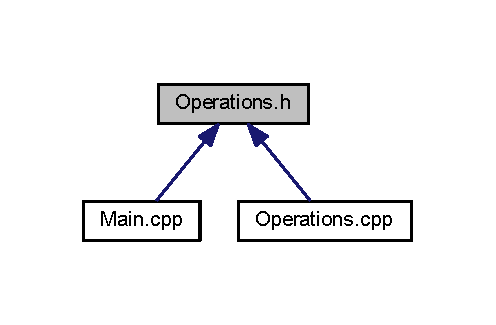
\includegraphics[width=238pt]{_operations_8h__dep__incl}
\end{center}
\end{figure}
\subsection*{Функции}
\begin{DoxyCompactItemize}
\item 
void \hyperlink{_operations_8h_a784c09041cf40075e8eb016a2d8419d6}{root} ()
\item 
bool \hyperlink{_operations_8h_a06ba6d957eba855cc9f88ce7ac641722}{b\+\_\+file\+\_\+exists} (const char $\ast$ch\+\_\+file\+\_\+name)
\item 
int \hyperlink{_operations_8h_a5f44f09549aae42fa22e71e761b40abc}{i\+\_\+checking\+\_\+files} ()
\item 
void \hyperlink{_operations_8h_a11b373fd61e18cd28810a5b607e1749a}{v\+\_\+initialization} ()
\end{DoxyCompactItemize}


\subsection{Подробное описание}
Заголовочный файл с вызовом модуля проверки стандартных файлов программы и вызова алгоритма рутирования. 

Вызов\+: 
\begin{DoxyCode}
\textcolor{keywordtype}{void} \hyperlink{_operations_8cpp_a784c09041cf40075e8eb016a2d8419d6}{root}();
\textcolor{keywordtype}{void} \hyperlink{_operations_8cpp_a11b373fd61e18cd28810a5b607e1749a}{v\_initialization}();
\end{DoxyCode}


\begin{DoxyAuthor}{Автор}
Sava\+Lione 
\end{DoxyAuthor}


\subsection{Функции}
\mbox{\Hypertarget{_operations_8h_a06ba6d957eba855cc9f88ce7ac641722}\label{_operations_8h_a06ba6d957eba855cc9f88ce7ac641722}} 
\index{Operations.\+h@{Operations.\+h}!b\+\_\+file\+\_\+exists@{b\+\_\+file\+\_\+exists}}
\index{b\+\_\+file\+\_\+exists@{b\+\_\+file\+\_\+exists}!Operations.\+h@{Operations.\+h}}
\subsubsection{\texorpdfstring{b\+\_\+file\+\_\+exists()}{b\_file\_exists()}}
{\footnotesize\ttfamily bool b\+\_\+file\+\_\+exists (\begin{DoxyParamCaption}\item[{const char $\ast$}]{ch\+\_\+file\+\_\+name }\end{DoxyParamCaption})}

Вызов модуля проверки файла на наличие в папке. 
\begin{DoxyParams}[1]{Аргументы}
\mbox{\tt in}  & {\em ch\+\_\+file\+\_\+name} & Путь и файл, для проверки. \\
\hline
\end{DoxyParams}
\begin{DoxyReturn}{Возвращает}
наличие файла. 
\end{DoxyReturn}


См. определение в файле Operations.\+cpp строка 54

\mbox{\Hypertarget{_operations_8h_a5f44f09549aae42fa22e71e761b40abc}\label{_operations_8h_a5f44f09549aae42fa22e71e761b40abc}} 
\index{Operations.\+h@{Operations.\+h}!i\+\_\+checking\+\_\+files@{i\+\_\+checking\+\_\+files}}
\index{i\+\_\+checking\+\_\+files@{i\+\_\+checking\+\_\+files}!Operations.\+h@{Operations.\+h}}
\subsubsection{\texorpdfstring{i\+\_\+checking\+\_\+files()}{i\_checking\_files()}}
{\footnotesize\ttfamily int i\+\_\+checking\+\_\+files (\begin{DoxyParamCaption}{ }\end{DoxyParamCaption})}

Вызов модуля проверки файлов. \begin{DoxyReturn}{Возвращает}
0 -\/ неуспешная проверка файлов. 1 -\/ успешная проверка файлов. 
\end{DoxyReturn}


См. определение в файле Operations.\+cpp строка 61

\mbox{\Hypertarget{_operations_8h_a784c09041cf40075e8eb016a2d8419d6}\label{_operations_8h_a784c09041cf40075e8eb016a2d8419d6}} 
\index{Operations.\+h@{Operations.\+h}!root@{root}}
\index{root@{root}!Operations.\+h@{Operations.\+h}}
\subsubsection{\texorpdfstring{root()}{root()}}
{\footnotesize\ttfamily void root (\begin{DoxyParamCaption}{ }\end{DoxyParamCaption})}

Вызов алгоритма рутирования. 

См. определение в файле Operations.\+cpp строка 38

\mbox{\Hypertarget{_operations_8h_a11b373fd61e18cd28810a5b607e1749a}\label{_operations_8h_a11b373fd61e18cd28810a5b607e1749a}} 
\index{Operations.\+h@{Operations.\+h}!v\+\_\+initialization@{v\+\_\+initialization}}
\index{v\+\_\+initialization@{v\+\_\+initialization}!Operations.\+h@{Operations.\+h}}
\subsubsection{\texorpdfstring{v\+\_\+initialization()}{v\_initialization()}}
{\footnotesize\ttfamily void v\+\_\+initialization (\begin{DoxyParamCaption}{ }\end{DoxyParamCaption})}

Функция проверяет наличие 3 стандартных файлов программы \begin{DoxyVerb}logger.log

rules.txt

settings.ini\end{DoxyVerb}
 

См. определение в файле Operations.\+cpp строка 108


\hypertarget{_settings_8cpp}{}\section{Файл Settings.\+cpp}
\label{_settings_8cpp}\index{Settings.\+cpp@{Settings.\+cpp}}


Модуль настроек. Парсит переменные в файлах.  


{\ttfamily \#include $<$fstream$>$}\newline
{\ttfamily \#include $<$string$>$}\newline
{\ttfamily \#include \char`\"{}../core/\+Constants.\+h\char`\"{}}\newline
Граф включаемых заголовочных файлов для Settings.\+cpp\+:
\nopagebreak
\begin{figure}[H]
\begin{center}
\leavevmode
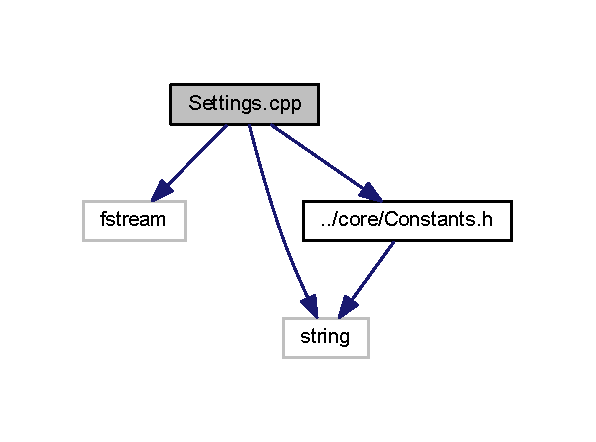
\includegraphics[width=286pt]{_settings_8cpp__incl}
\end{center}
\end{figure}
\subsection*{Функции}
\begin{DoxyCompactItemize}
\item 
bool \hyperlink{_settings_8cpp_a7fcd42142e325cb27a380f49d655f9de}{b\+\_\+settings} (char ch\+\_\+arr\+\_\+value\mbox{[}$\,$\mbox{]})
\end{DoxyCompactItemize}


\subsection{Подробное описание}
Модуль настроек. Парсит переменные в файлах. 

\begin{DoxyAuthor}{Автор}
Sava\+Lione 
\end{DoxyAuthor}


\subsection{Функции}
\mbox{\Hypertarget{_settings_8cpp_a7fcd42142e325cb27a380f49d655f9de}\label{_settings_8cpp_a7fcd42142e325cb27a380f49d655f9de}} 
\index{Settings.\+cpp@{Settings.\+cpp}!b\+\_\+settings@{b\+\_\+settings}}
\index{b\+\_\+settings@{b\+\_\+settings}!Settings.\+cpp@{Settings.\+cpp}}
\subsubsection{\texorpdfstring{b\+\_\+settings()}{b\_settings()}}
{\footnotesize\ttfamily bool b\+\_\+settings (\begin{DoxyParamCaption}\item[{char}]{ch\+\_\+arr\+\_\+value\mbox{[}$\,$\mbox{]} }\end{DoxyParamCaption})}

Парсинг параметров 
\begin{DoxyParams}[1]{Аргументы}
\mbox{\tt in}  & {\em ch\+\_\+arr\+\_\+value\mbox{[}$\,$\mbox{]}} & Значение, которое надо найти в файле. \\
\hline
\end{DoxyParams}
\begin{DoxyReturn}{Возвращает}
Значение переменной true false 
\end{DoxyReturn}
\begin{Desc}
\item[Примеры\+: ]\par
\hyperlink{settings_8cpp-example}{settings.\+cpp}.\end{Desc}


См. определение в файле Settings.\+cpp строка 22


\hypertarget{_settings_8h}{}\section{Файл Settings.\+h}
\label{_settings_8h}\index{Settings.\+h@{Settings.\+h}}


Заголовочный файл с подключением модуля настроек.  


Граф файлов, в которые включается этот файл\+:
\nopagebreak
\begin{figure}[H]
\begin{center}
\leavevmode
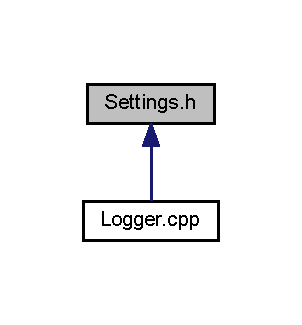
\includegraphics[width=145pt]{_settings_8h__dep__incl}
\end{center}
\end{figure}
\subsection*{Функции}
\begin{DoxyCompactItemize}
\item 
bool \hyperlink{_settings_8h_a7fcd42142e325cb27a380f49d655f9de}{b\+\_\+settings} (char ch\+\_\+arr\+\_\+value\mbox{[}$\,$\mbox{]})
\end{DoxyCompactItemize}


\subsection{Подробное описание}
Заголовочный файл с подключением модуля настроек. 



\subsection{Функции}
\mbox{\Hypertarget{_settings_8h_a7fcd42142e325cb27a380f49d655f9de}\label{_settings_8h_a7fcd42142e325cb27a380f49d655f9de}} 
\index{Settings.\+h@{Settings.\+h}!b\+\_\+settings@{b\+\_\+settings}}
\index{b\+\_\+settings@{b\+\_\+settings}!Settings.\+h@{Settings.\+h}}
\subsubsection{\texorpdfstring{b\+\_\+settings()}{b\_settings()}}
{\footnotesize\ttfamily bool b\+\_\+settings (\begin{DoxyParamCaption}\item[{char}]{ch\+\_\+arr\+\_\+value\mbox{[}$\,$\mbox{]} }\end{DoxyParamCaption})}

Парсинг параметров 
\begin{DoxyParams}[1]{Аргументы}
\mbox{\tt in}  & {\em ch\+\_\+arr\+\_\+value\mbox{[}$\,$\mbox{]}} & Значение, которое надо найти в файле \\
\hline
\end{DoxyParams}
\begin{DoxyReturn}{Возвращает}
Значение переменной true false 
\end{DoxyReturn}


См. определение в файле Settings.\+cpp строка 22


\hypertarget{_templates_8cpp}{}\section{Файл Templates.\+cpp}
\label{_templates_8cpp}\index{Templates.\+cpp@{Templates.\+cpp}}


Функции для создания стандартных файлов программы.  


{\ttfamily \#include $<$fstream$>$}\newline
{\ttfamily \#include \char`\"{}Templates.\+h\char`\"{}}\newline
{\ttfamily \#include \char`\"{}..\textbackslash{}core\textbackslash{}\+Constants.\+h\char`\"{}}\newline
Граф включаемых заголовочных файлов для Templates.\+cpp\+:
\nopagebreak
\begin{figure}[H]
\begin{center}
\leavevmode
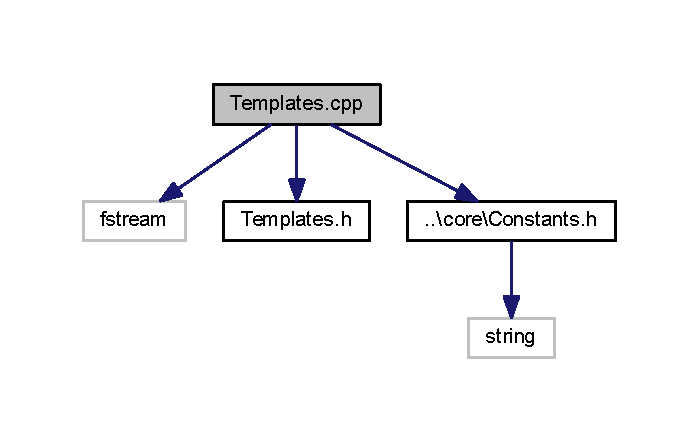
\includegraphics[width=336pt]{_templates_8cpp__incl}
\end{center}
\end{figure}
\subsection*{Функции}
\begin{DoxyCompactItemize}
\item 
void \hyperlink{_templates_8cpp_abeb0b4d4d31b9c74744a0b9881d95066}{v\+\_\+templates\+\_\+create\+\_\+logger\+\_\+log} ()
\item 
void \hyperlink{_templates_8cpp_a593e33d5988d6a49d581f52d94471895}{v\+\_\+templates\+\_\+create\+\_\+settings\+\_\+ini} ()
\end{DoxyCompactItemize}


\subsection{Подробное описание}
Функции для создания стандартных файлов программы. 



\subsection{Функции}
\mbox{\Hypertarget{_templates_8cpp_abeb0b4d4d31b9c74744a0b9881d95066}\label{_templates_8cpp_abeb0b4d4d31b9c74744a0b9881d95066}} 
\index{Templates.\+cpp@{Templates.\+cpp}!v\+\_\+templates\+\_\+create\+\_\+logger\+\_\+log@{v\+\_\+templates\+\_\+create\+\_\+logger\+\_\+log}}
\index{v\+\_\+templates\+\_\+create\+\_\+logger\+\_\+log@{v\+\_\+templates\+\_\+create\+\_\+logger\+\_\+log}!Templates.\+cpp@{Templates.\+cpp}}
\subsubsection{\texorpdfstring{v\+\_\+templates\+\_\+create\+\_\+logger\+\_\+log()}{v\_templates\_create\_logger\_log()}}
{\footnotesize\ttfamily void v\+\_\+templates\+\_\+create\+\_\+logger\+\_\+log (\begin{DoxyParamCaption}{ }\end{DoxyParamCaption})}

Создание файла пользовательского соглашения. \begin{DoxyVerb}logger.log - файл с логом вывода\end{DoxyVerb}
 \begin{Desc}
\item[Примеры\+: ]\par
\hyperlink{templates_8cpp-example}{templates.\+cpp}.\end{Desc}


См. определение в файле Templates.\+cpp строка 22

\mbox{\Hypertarget{_templates_8cpp_a593e33d5988d6a49d581f52d94471895}\label{_templates_8cpp_a593e33d5988d6a49d581f52d94471895}} 
\index{Templates.\+cpp@{Templates.\+cpp}!v\+\_\+templates\+\_\+create\+\_\+settings\+\_\+ini@{v\+\_\+templates\+\_\+create\+\_\+settings\+\_\+ini}}
\index{v\+\_\+templates\+\_\+create\+\_\+settings\+\_\+ini@{v\+\_\+templates\+\_\+create\+\_\+settings\+\_\+ini}!Templates.\+cpp@{Templates.\+cpp}}
\subsubsection{\texorpdfstring{v\+\_\+templates\+\_\+create\+\_\+settings\+\_\+ini()}{v\_templates\_create\_settings\_ini()}}
{\footnotesize\ttfamily void v\+\_\+templates\+\_\+create\+\_\+settings\+\_\+ini (\begin{DoxyParamCaption}{ }\end{DoxyParamCaption})}

Создание файла настроек. \begin{DoxyVerb}settings.ini - файл с настройками\end{DoxyVerb}
 \begin{Desc}
\item[Примеры\+: ]\par
\hyperlink{templates_8cpp-example}{templates.\+cpp}.\end{Desc}


См. определение в файле Templates.\+cpp строка 42


\hypertarget{_templates_8h}{}\section{Файл Templates.\+h}
\label{_templates_8h}\index{Templates.\+h@{Templates.\+h}}


Заголовочный файл с подключением модуля создания стандартных файлов программы.  


Граф файлов, в которые включается этот файл\+:
\nopagebreak
\begin{figure}[H]
\begin{center}
\leavevmode
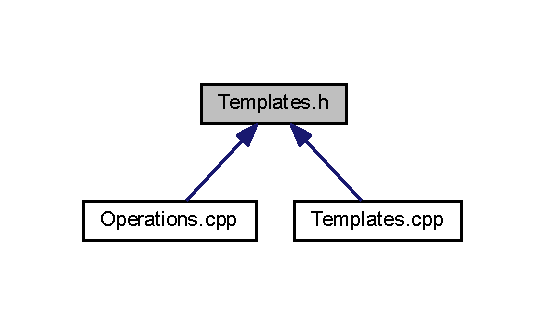
\includegraphics[width=262pt]{_templates_8h__dep__incl}
\end{center}
\end{figure}
\subsection*{Функции}
\begin{DoxyCompactItemize}
\item 
void \hyperlink{_templates_8h_abeb0b4d4d31b9c74744a0b9881d95066}{v\+\_\+templates\+\_\+create\+\_\+logger\+\_\+log} ()
\item 
void \hyperlink{_templates_8h_a593e33d5988d6a49d581f52d94471895}{v\+\_\+templates\+\_\+create\+\_\+settings\+\_\+ini} ()
\end{DoxyCompactItemize}


\subsection{Подробное описание}
Заголовочный файл с подключением модуля создания стандартных файлов программы. 

\begin{DoxyAuthor}{Автор}
Sava\+Lione 
\end{DoxyAuthor}


\subsection{Функции}
\mbox{\Hypertarget{_templates_8h_abeb0b4d4d31b9c74744a0b9881d95066}\label{_templates_8h_abeb0b4d4d31b9c74744a0b9881d95066}} 
\index{Templates.\+h@{Templates.\+h}!v\+\_\+templates\+\_\+create\+\_\+logger\+\_\+log@{v\+\_\+templates\+\_\+create\+\_\+logger\+\_\+log}}
\index{v\+\_\+templates\+\_\+create\+\_\+logger\+\_\+log@{v\+\_\+templates\+\_\+create\+\_\+logger\+\_\+log}!Templates.\+h@{Templates.\+h}}
\subsubsection{\texorpdfstring{v\+\_\+templates\+\_\+create\+\_\+logger\+\_\+log()}{v\_templates\_create\_logger\_log()}}
{\footnotesize\ttfamily void v\+\_\+templates\+\_\+create\+\_\+logger\+\_\+log (\begin{DoxyParamCaption}{ }\end{DoxyParamCaption})}

Создание файла пользовательского соглашения. \begin{DoxyVerb}logger.log - файл с логом вывода.\end{DoxyVerb}


Создание файла пользовательского соглашения. \begin{DoxyVerb}logger.log - файл с логом вывода\end{DoxyVerb}
 

См. определение в файле Templates.\+cpp строка 24

\mbox{\Hypertarget{_templates_8h_a593e33d5988d6a49d581f52d94471895}\label{_templates_8h_a593e33d5988d6a49d581f52d94471895}} 
\index{Templates.\+h@{Templates.\+h}!v\+\_\+templates\+\_\+create\+\_\+settings\+\_\+ini@{v\+\_\+templates\+\_\+create\+\_\+settings\+\_\+ini}}
\index{v\+\_\+templates\+\_\+create\+\_\+settings\+\_\+ini@{v\+\_\+templates\+\_\+create\+\_\+settings\+\_\+ini}!Templates.\+h@{Templates.\+h}}
\subsubsection{\texorpdfstring{v\+\_\+templates\+\_\+create\+\_\+settings\+\_\+ini()}{v\_templates\_create\_settings\_ini()}}
{\footnotesize\ttfamily void v\+\_\+templates\+\_\+create\+\_\+settings\+\_\+ini (\begin{DoxyParamCaption}{ }\end{DoxyParamCaption})}

Создание файла настроек. \begin{DoxyVerb}settings.ini - файл с настройками.\end{DoxyVerb}


Создание файла настроек. \begin{DoxyVerb}settings.ini - файл с настройками\end{DoxyVerb}
 

См. определение в файле Templates.\+cpp строка 41


\chapter{Примеры}
\hypertarget{color_8cpp-example}{}\section{color.\+cpp}
\begin{DoxyAuthor}{Автор}
Sava\+Lione
\end{DoxyAuthor}

\begin{DoxyCodeInclude}
\textcolor{preprocessor}{#include "..\(\backslash\)core\(\backslash\)Color.h"}

\textcolor{keywordtype}{int} \hyperlink{_main_8cpp_ae66f6b31b5ad750f1fe042a706a4e3d4}{main}() \{
    \hyperlink{_color_8cpp_a8bfe4542d1f10bae3f4ff0ec688aa67f}{v\_set\_color}(\hyperlink{_color_8h_a37dbdc30935031c05304482e1be89d8fa35d6719cb4d7577c031b3d79057a1b79}{BLUE}, \hyperlink{_color_8h_a37dbdc30935031c05304482e1be89d8fa283fc479650da98250635b9c3c0e7e50}{WHITE});
    
    \hyperlink{_color_8cpp_a8bfe4542d1f10bae3f4ff0ec688aa67f}{v\_set\_color}(\hyperlink{_color_8h_a37dbdc30935031c05304482e1be89d8faa60bd322f93178d68184e30e162571ca}{GREEN});
    
    \hyperlink{_color_8cpp_a8bfe4542d1f10bae3f4ff0ec688aa67f}{v\_set\_color}();
    
    \textcolor{keywordflow}{return} 0;
\}
\end{DoxyCodeInclude}
 
\hypertarget{constants_8cpp-example}{}\section{constants.\+cpp}
\begin{DoxyAuthor}{Автор}
Sava\+Lione
\end{DoxyAuthor}

\begin{DoxyCodeInclude}
\textcolor{preprocessor}{#include <iostream>}

\textcolor{preprocessor}{#include "..\(\backslash\)core\(\backslash\)Constants.h"}

\textcolor{keywordtype}{int} \hyperlink{_main_8cpp_ae66f6b31b5ad750f1fe042a706a4e3d4}{main}() \{
    \textcolor{comment}{// The user continued the program despite the error.}
    std::cout << \hyperlink{namespaceradix_ad5e76eca849713be360ed8478545d801}{radix::ch\_user\_continue} << std::endl;
    \textcolor{keywordflow}{return} 0;
\}
\end{DoxyCodeInclude}
 
\hypertarget{items_8cpp-example}{}\section{items.\+cpp}
\begin{DoxyAuthor}{Автор}
Sava\+Lione
\end{DoxyAuthor}

\begin{DoxyCodeInclude}
\textcolor{preprocessor}{#include <iostream>}

\textcolor{preprocessor}{#include "..\(\backslash\)ui\(\backslash\)Items.h"}

\textcolor{keyword}{using namespace }\hyperlink{namespacestd}{std};

\textcolor{keywordtype}{int} \hyperlink{_main_8cpp_ae66f6b31b5ad750f1fe042a706a4e3d4}{main}() \{
    cout << \hyperlink{_items_8cpp_afb16d6cecac9a7da7edd9389097a74b2}{s\_mainmenu}() << endl;
    cout << \hyperlink{_items_8cpp_a45daa1eafaa5c4d1e9246abdd4db144e}{s\_querymenu}(\textcolor{stringliteral}{"String"}) << endl;
    cout << \hyperlink{_items_8cpp_acda300061b64b7f3003c9103cfb1bb19}{s\_checkagreement}() << endl;
    \hyperlink{_items_8cpp_ae0f9a7fdce9e3a275336f70656c0c4fc}{v\_manual}();
    \textcolor{keywordflow}{return} 0;
\}
\end{DoxyCodeInclude}
 
\hypertarget{log_8cpp-example}{}\section{log.\+cpp}
\begin{DoxyAuthor}{Автор}
Sava\+Lione
\end{DoxyAuthor}

\begin{DoxyCodeInclude}
\textcolor{preprocessor}{#include "..\(\backslash\)io\(\backslash\)Logger.h"}

\textcolor{keywordtype}{int} \hyperlink{_main_8cpp_ae66f6b31b5ad750f1fe042a706a4e3d4}{main}() \{
    \hyperlink{_logger_8cpp_a85cbef1702d055318336f0f3a5036959}{log}(\textcolor{stringliteral}{"LOG"}, \textcolor{stringliteral}{"Hello World!!!"});
    \textcolor{keywordflow}{return} 0;
\}
\end{DoxyCodeInclude}
 
\hypertarget{menu_8cpp-example}{}\section{menu.\+cpp}
\begin{DoxyAuthor}{Автор}
Sava\+Lione
\end{DoxyAuthor}

\begin{DoxyCodeInclude}
\textcolor{preprocessor}{#include <iostream>}

\textcolor{preprocessor}{#include "..\(\backslash\)ui\(\backslash\)Menu.h"}

\textcolor{keyword}{using namespace }\hyperlink{namespacestd}{std};

\textcolor{keywordtype}{void} before();
\textcolor{keywordtype}{void} after();

\textcolor{keywordtype}{int} \hyperlink{_main_8cpp_ae66f6b31b5ad750f1fe042a706a4e3d4}{main}() \{
    \hyperlink{structmenu__s}{menu\_s} testmenu;
    testmenu.\hyperlink{structmenu__s_a2b4d6cd699b46daba2bb8297c11971aa}{name} = \textcolor{stringliteral}{"Test menu"};
    testmenu.\hyperlink{structmenu__s_ad653d55a31d8503ad989ffd0b94c14e4}{s\_before} = \textcolor{stringliteral}{"Test before."};
    testmenu.\hyperlink{structmenu__s_a8622e3ccae9b1356ad3e2e3eb51a44e8}{s\_after} = \textcolor{stringliteral}{"Test after."};
    testmenu.\hyperlink{structmenu__s_abf8d2985fb3bf50d8e2075701149375a}{vec\_item\_name} = \{\textcolor{stringliteral}{"Test"}, \textcolor{stringliteral}{"Exit"}\};
    testmenu.\hyperlink{structmenu__s_aa71bffe8004873d1f43eeeb4e17595c8}{before\_menu} = before;
    testmenu.\hyperlink{structmenu__s_ad0e4cb85e66d3c8bc25687a92d986939}{after\_menu} = after;
    cout << \hyperlink{_menu_8cpp_a20a38c5c97dbebd634a7b5c71fcd6120}{s\_menu}(mainmenu) << endl;
    \textcolor{keywordflow}{return} 0;
\}

\textcolor{keywordtype}{void} before() \{
    cout << \textcolor{stringliteral}{"Before."} << endl;
\}

\textcolor{keywordtype}{void} after() \{
    cout << \textcolor{stringliteral}{"After."} << endl;
\}
\end{DoxyCodeInclude}
 
\hypertarget{_operations_8cpp-example}{}\section{Operations.\+cpp}

\begin{DoxyCodeInclude}
\textcolor{preprocessor}{#include "..\(\backslash\)core\(\backslash\)Operations.h"}

\textcolor{keywordtype}{int} \hyperlink{_main_8cpp_ae66f6b31b5ad750f1fe042a706a4e3d4}{main}() \{
    \hyperlink{_operations_8cpp_a784c09041cf40075e8eb016a2d8419d6}{root}();
    \textcolor{keywordflow}{return} \hyperlink{_operations_8cpp_a5f44f09549aae42fa22e71e761b40abc}{i\_checking\_files}();
\}
\end{DoxyCodeInclude}
 
\hypertarget{_operations__initialization_8cpp-example}{}\section{Operations\+\_\+\+Initialization.\+cpp}
\begin{DoxyAuthor}{Автор}
Sava\+Lione
\end{DoxyAuthor}

\begin{DoxyCodeInclude}
\textcolor{preprocessor}{#include "..\(\backslash\)core\(\backslash\)Operations.h"}

\textcolor{keywordtype}{int} \hyperlink{_main_8cpp_ae66f6b31b5ad750f1fe042a706a4e3d4}{main}() \{
    \textcolor{keyword}{const} \textcolor{keywordtype}{char} ch\_radix\_exe[] = \textcolor{stringliteral}{"Radix.exe"};
    \textcolor{keywordflow}{if} (\hyperlink{_operations_8cpp_a06ba6d957eba855cc9f88ce7ac641722}{b\_file\_exists}(ch\_radix\_exe[])) \{
        \textcolor{comment}{// File found}
    \} \textcolor{keywordflow}{else} \{
        \textcolor{comment}{// File not found}
    \}
    
    \textcolor{keywordflow}{if} (\hyperlink{_operations_8cpp_a5f44f09549aae42fa22e71e761b40abc}{i\_checking\_files}() == 1) \{
        \textcolor{comment}{// Successful file verification}
    \} \textcolor{keywordflow}{else} \{
        \textcolor{comment}{// Unsuccessful file check.}
    \}
    \hyperlink{_operations_8cpp_a11b373fd61e18cd28810a5b607e1749a}{v\_initialization}();
    \textcolor{keywordflow}{return} 0;
\}
\end{DoxyCodeInclude}
 
\hypertarget{settings_8cpp-example}{}\section{settings.\+cpp}
\begin{DoxyAuthor}{Автор}
Sava\+Lione
\end{DoxyAuthor}

\begin{DoxyCodeInclude}
\textcolor{preprocessor}{#include "..\(\backslash\)io\(\backslash\)Settings.h"}

\textcolor{keywordtype}{int} \hyperlink{_main_8cpp_ae66f6b31b5ad750f1fe042a706a4e3d4}{main}() \{
    \textcolor{keywordflow}{if} (\hyperlink{_settings_8cpp_a7fcd42142e325cb27a380f49d655f9de}{b\_settings}(\textcolor{stringliteral}{"rules"})) \{
        \textcolor{comment}{// rules = true}
    \}
    \textcolor{keywordflow}{return} 0;
\}
\end{DoxyCodeInclude}
 
\hypertarget{templates_8cpp-example}{}\section{templates.\+cpp}
\begin{DoxyAuthor}{Автор}
Sava\+Lione
\end{DoxyAuthor}

\begin{DoxyCodeInclude}
\textcolor{preprocessor}{#include "..\(\backslash\)io\(\backslash\)Templates.h"}

\textcolor{keywordtype}{int} \hyperlink{_main_8cpp_ae66f6b31b5ad750f1fe042a706a4e3d4}{main}() \{
    \hyperlink{_templates_8cpp_abeb0b4d4d31b9c74744a0b9881d95066}{v\_templates\_create\_logger\_log}();
    v\_templates\_create\_rules\_txt();
    \hyperlink{_templates_8cpp_a593e33d5988d6a49d581f52d94471895}{v\_templates\_create\_settings\_ini}();
    \textcolor{keywordflow}{return} 0;
\}
\end{DoxyCodeInclude}
 
%--- End generated contents ---

% Index
\backmatter
\newpage
\phantomsection
\clearemptydoublepage
\addcontentsline{toc}{chapter}{Алфавитный указатель}
\printindex

\end{document}
